\documentclass[11pt,oneside]{book}
\usepackage{fontspec}
\usepackage{xeCJK}
\setmainfont{Latin Modern Roman}
\setCJKmainfont[ItalicFont={Noto Serif CJK TC},BoldItalicFont={Noto Serif CJK TC Bold}]{Noto Serif CJK TC}
\setCJKsansfont{Noto Sans CJK TC}
\setCJKmonofont{Noto Sans Mono CJK TC}
\newfontfamily\proseunicodefont{DejaVu Serif}
\usepackage[margin=1in]{geometry}
\usepackage{microtype}
\usepackage{amsmath,amssymb,amsthm,mathtools,bm}
\usepackage{graphicx}
\usepackage{xcolor}
\usepackage{booktabs}
\usepackage{array}
\usepackage{longtable}
\usepackage{enumitem}
\usepackage{float}
\usepackage{caption}
\usepackage{hyperref}
\usepackage{fancyhdr}
\usepackage{tikz}
\usetikzlibrary{arrows.meta,positioning,calc,decorations.pathmorphing}

\hypersetup{
  colorlinks=true,
  linkcolor=blue!50!black,
  urlcolor=blue!50!black,
  citecolor=blue!50!black
}

\setlength{\parskip}{0.5em}
\setlength{\parindent}{0pt}
\setlist[itemize]{topsep=0.25em,itemsep=0.2em}
\setlist[enumerate]{topsep=0.25em,itemsep=0.2em}
\setlength{\headheight}{40pt}
\numberwithin{equation}{chapter}

\newtheorem{theorem}{定理}[chapter]
\newtheorem{proposition}[theorem]{命題}
\newtheorem{lemma}[theorem]{引理}
\newtheorem{corollary}[theorem]{推論}
\theoremstyle{definition}
\newtheorem{definition}[theorem]{定義}
\newtheorem{example}[theorem]{例}
\theoremstyle{remark}
\newtheorem{remark}[theorem]{註}

\providecommand{\ket}[1]{\left\lvert#1\right\rangle}
\providecommand{\bra}[1]{\left\langle#1\right\rvert}
\providecommand{\braket}[2]{\left\langle#1\,\middle|\,#2\right\rangle}
\providecommand{\expect}[1]{\left\langle#1\right\rangle}
\newcommand{\lectureoverview}[1]{\paragraph{概述。} #1}
\newenvironment{classroomqa}{%
  \par\medskip
  \begin{minipage}{0.96\textwidth}
}{%
  \end{minipage}
  \par\medskip
}
\newcommand{\audiencequestion}[1]{\noindent\textbf{聽眾提問。} #1\par\smallskip}
\newcommand{\lecturerresponse}[1]{\noindent\textbf{回答。} #1\par}
\newcommand{\lecturetimestamp}[1]{\footnote{講課時間： #1.}}
\newcommand{\lectureframe}[1]{\par\smallskip{\centering\footnotesize\itshape 講課畫面： #1.\par}}
\newcommand{\editorialnote}[1]{\footnote{編者說明： #1}}

\makeatletter
\newcommand{\course@headerfont}{\normalfont\small\itshape}
\newcommand{\course@pagefont}{\normalfont\small}
\newcommand{\course@headerraise}{14pt}
\newlength{\course@headerboxheight}
\setlength{\course@headerboxheight}{\dimexpr\headheight-\course@headerraise-9pt\relax}
\newcommand{\course@leftheadbox}[1]{%
  \raisebox{\course@headerraise}{%
    \parbox[t][\course@headerboxheight][t]{0.82\textwidth}{%
      \raggedright\course@headerfont\strut\MakeUppercase{#1}\strut%
    }%
  }%
}
\newcommand{\course@rightheadbox}[1]{%
  \raisebox{\course@headerraise}{%
    \parbox[t][\course@headerboxheight][t]{0.82\textwidth}{%
      \raggedleft\course@headerfont\strut\MakeUppercase{#1}\strut%
    }%
  }%
}
\renewcommand{\chaptermark}[1]{\markboth{\MakeUppercase{\chaptername\ \thechapter.\ #1}}{}}
\renewcommand{\sectionmark}[1]{\markright{\MakeUppercase{\thesection\hspace{0.4em}#1}}}
\fancyhf{}
\fancyhead[L]{\course@leftheadbox{\leftmark}}
\fancyhead[R]{\course@pagefont\thepage}
\renewcommand{\headrulewidth}{0.5pt}
\pagestyle{fancy}
\fancypagestyle{plain}{%
  \fancyhf{}
  \fancyhead[L]{\course@leftheadbox{\leftmark}}
  \fancyhead[R]{\course@pagefont\thepage}
  \renewcommand{\headrulewidth}{0.5pt}
}
\makeatother

\renewcommand{\contentsname}{目錄}
\renewcommand{\chaptername}{章}
\renewcommand{\figurename}{圖}
\renewcommand{\tablename}{表}
\renewcommand{\proofname}{證明}
\renewcommand{\bibname}{參考文獻}
\emergencystretch=2em
\pdfstringdefDisableCommands{\def\proseunicodefont{}}

\geometry{paperwidth=177.6mm,paperheight=252mm,left=16mm,right=16mm,
 top=18mm,bottom=18mm,includeheadfoot,headheight=28pt,headsep=7mm,footskip=9mm}
\usepackage{scrextend}
\changefontsizes[17pt]{12pt}
\raggedbottom
\renewenvironment{classroomqa}{\par\medskip\begingroup}{\par\endgroup\medskip}
\fancyhf{}
\setlength{\headwidth}{\textwidth}
\fancyhead[L]{\parbox{\textwidth}{\raggedright\fontsize{9}{11}\selectfont\nouppercase{\leftmark}}}
\fancyfoot[C]{\small\thepage}
\renewcommand{\headrulewidth}{0.3pt}
\fancypagestyle{plain}{\fancyhf{}\fancyfoot[C]{\small\thepage}\renewcommand{\headrulewidth}{0pt}}

\hypersetup{
  pdftitle={Quantum Entanglement, Part 3},
  pdfauthor={Lectures by Leonard Susskind; companion edition by LazyingArt LLC},
  pdfsubject={Independently edited companion notes for the 2006 Fall lecture course},
  pdfcreator={LaTeX with hyperref}
}
\graphicspath{{../../../generated_course_notes/supplementary/quantum_entanglement/2006_fall_part_3/figures/}{../../../generated_course_notes/supplementary/quantum_entanglement/2006_fall_part_3/assets/}}
\begin{document}
\frontmatter
\hypersetup{pageanchor=false}
\begin{titlepage}
\hyphenpenalty=10000\exhyphenpenalty=10000
\thispagestyle{empty}
\begin{tikzpicture}[remember picture,overlay]
  \node[anchor=center,inner sep=0] at (current page.center) {%
    \includegraphics[height=\paperheight,keepaspectratio]{../../../generated_course_notes/supplementary/quantum_entanglement/2006_fall_part_3/assets/cover-art.png}%
  };
  \node[
    anchor=north west,
    align=left,
    text width=0.78\paperwidth,
    fill=white,
    fill opacity=0.9,
    rounded corners=8pt,
    inner xsep=10pt,
    inner ysep=8pt
  ] at ([xshift=0.08\paperwidth,yshift=-0.06\paperheight]current page.north west) {%
    {\fontsize{30}{33}\selectfont\bfseries\color{black!88} 量子糾纏：第三部分\\[0.85em]}
    {\large\color{black!72} 繁體中文版 / 2006年秋季・第3部分}
  };
  \node[
    anchor=south west,
    align=left,
    text width=0.68\paperwidth,
    fill=white,
    fill opacity=0.82,
    text opacity=1,
    rounded corners=6pt,
    inner sep=12pt
  ] at ([xshift=0.08\paperwidth,yshift=0.08\paperheight]current page.south west) {%
    {\normalsize\color{black!78} 原講授：Leonard Susskind\\[0.35em]}
    {\small\color{black!72} 講義輔助版本：\href{https://lazying.art}{LazyingArt LLC} / \href{https://github.com/lachlanchen/Video2Book}{Video2Book}}
  };
\end{tikzpicture}
\mbox{}
\end{titlepage}
\hypersetup{pageanchor=true}

\clearpage
\chapter*{關於本筆記}
這些經獨立編輯的配套筆記，依據 Leonard Susskind 的 2006 年量子糾纏講座課程第三部分編寫。筆記內容根據機器轉錄稿、字幕及精選的黑板畫面重建，並對照可取得的原始資料加以核對。這些筆記並非 Susskind 教授的原始手稿，也未經他審閱或認可。

本版本由 \href{https://lazying.art}{LazyingArt LLC} 使用開源 \href{https://github.com/lachlanchen/Video2Book}{Video2Book} 工具製作。機器轉錄稿另有提供，但可能含有辨識錯誤。編輯上的說明及較具實質性的重建均於註腳標示。
\clearpage
\tableofcontents
\mainmatter
\chapter{狹義相對論：參考系、同時性與洛倫茲變換}

相對論原理指出，物理定律不因我們用哪個慣性參考系描述它們而改變。我們首先要處理運動學：空間、時間、運動、同步，以及從一個慣性參考系轉換到另一個參考系的意義。接著才是動力學，包括相對論的能量、動量、力、相當於牛頓運動方程的方程，以及\(E=mc^2\)的意義。掌握這套架構後，我們就能從概念上探討廣義相對論，包括彎曲時空、粒子在指定引力場中的運動、黑洞，以及宇宙膨脹，而不必一開始就面對求解愛因斯坦場方程這個困難問題。

概念上的嚴謹與數學上的嚴謹，值得加以區分。我們不會採用明知不正確的近似；我們會著重說明引力場如何影響時鐘、粒子與幾何，同時暫緩介紹構造場方程任意解所需的數學工具。狹義相對論則必須更明確地處理，因為後續所有推理都以它的運動學為基礎。

因此，合適的起點不是某個著名公式，而是精確說明觀察者所說的位置和時間究竟是什麼意思。

\section{參考系是物理座標系}

想像空間中布滿了任意精細的米尺格架。每個格點都標上三個空間座標，而且每個格點上都有一個時鐘。這些尺和時鐘共同構成一個參考系。

\begin{definition}
\emph{事件}是指在某個位置、某個時刻發生的事情。在一維空間中，事件的座標寫作\((x,t)\)；在三維空間中則寫作\((x,y,z,t)\)。
\end{definition}

牛頓物理學還加入了一個強而有力的假設：所有理想時鐘都能一次同步，之後始終保持同步。時間是普遍的。時鐘可以移動，觀察者也可以帶著手錶，但所有人都被假定在任何地方都同意同一個\(t\)。這有時稱為絕對時間；可以把它想成上帝的時間，也就是一個適用於整個世界的時鐘。

相對論原理早於愛因斯坦。可以想像一列火車在完美平滑的鐵軌上勻速行駛，車廂裡沒有嘎嘎聲，也沒有震動。在車廂內拋球、接球，和在停靠車站的火車裡做起來完全一樣。拋接球是個出乎意料地完整的小型力學實驗：它需要掌握時間、重力、對準位置，並反覆控制軌跡。如果火車等速度行駛，這些規則就不會改變。向上直拋的球會回到同一隻手中；火車不會從球下方滑走。伽利略認識到這個事實，牛頓則在運動定律中有系統地表述了它。

伽利略之前，人們很容易推想：球在空中時，行進中的火車會繼續前進，因此拋接球的人必須向後或向前伸手才能接住球。這個推理忽略了球離手時已經具有火車的水平速度。只在平穩行駛的車廂內進行實驗，無法找出某種特殊的絕對靜止狀態。只有兩列火車之間的相對運動可以觀測。

因此，靜止的火車與等速度行駛的火車是兩個慣性參考系。在愛因斯坦之前，人們用伽利略變換來描述它們之間的關係。

\section{繪製時空圖}

暫且省略\(y\)和\(z\)，把時間畫在垂直方向，把位置\(x\)畫在水平方向。圖上的每個點都是一個事件。直線\(x=0\)是空間原點的歷史，也就是它的\emph{世界線}。相鄰的垂直線\(x=1,2,3,\ldots\)則是其他格點的世界線。水平線表示時間相同的一組事件。

\begin{figure}[H]
\centering
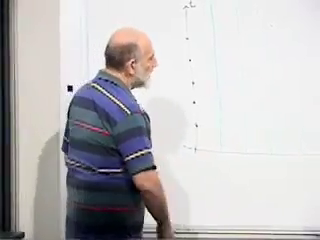
\includegraphics[width=0.62\textwidth]{lecture_01_figure_02.png}
\caption{靜止參考系的時間軸，以及空間格架最初幾個格點的世界線。}
\lectureframe{00:16:38}
\end{figure}

用理想化的圖來呈現，相同的構造會更清楚：

\begin{figure}[H]
\centering
\begin{tikzpicture}[scale=0.95]
\draw[->] (-1.2,0) -- (5.2,0) node[right] {$x$};
\draw[->] (0,-0.2) -- (0,4.8) node[above] {$t$};
\foreach \x in {-1,1,2,3,4}
  \draw[gray!65] (\x,0) -- (\x,4.4);
\foreach \y in {1,2,3,4}
  \draw[gray!65] (-1.0,\y) -- (4.4,\y);
\fill (0,0) circle (1.5pt);
\node[below left] at (0,0) {$0$};
\node[left] at (0,1) {$1$};
\node[left] at (0,2) {$2$};
\node[left] at (0,3) {$3$};
\node[below] at (1,0) {$1$};
\node[below] at (2,0) {$2$};
\node[below] at (3,0) {$3$};
\end{tikzpicture}
\caption{靜止的時空格架。垂直線表示位置不變；水平線表示時間不變。}
\end{figure}

格網是想像出來的，間距可以任意設定。我們可以用公尺、厘米、微米，或任何更小且有物理意義的間隔。格網的用途，是為每個事件指定精確的座標。

「參考系」一詞現在有了可操作的意義。它不只是某種觀點，也不是某個朝特定方向觀看的人；它是一套延展於空間中的座標裝置。給定一個事件，當地的尺規指出事件發生的位置，當地的時鐘指出事件發生的時刻。如此一來，我們就能比較不同參考系中的其他物理量：粒子的位置和速度、粒子的能量，也許還有物體的溫度，最後則是動量和力。最簡單的比較涉及\(x\)和\(t\)，所以我們從這裡開始。

現在，在一列以定速度\(v\)沿\(x\)正方向行駛的火車上設置第二套格架。選定兩個原點在\(t=0\)時重合。接著，運動中的原點沿著下式的世界線移動：
\begin{equation}
x=vt.
\end{equation}
固定在火車上的其他格點，也沿著彼此平行而傾斜的世界線移動。這種傾斜只是以幾何方式表示火車的位置隨時間改變。

假設火車尾端的格點是帶撇號的原點。在\(t=0\)時，它與車站原點重合。到了較晚的時刻\(t\)，它在車站參考系中的座標是\(vt\)。因此，座標為\(x\)的鄰近事件，距離火車原點只有\(x-vt\)。這說明了變換中為什麼要相減，而不是任意套用一條代數規則。

令\((x,t)\)表示事件在車站參考系中的座標，\((x',t')\)表示它在火車參考系中的座標。伽利略和牛頓的理論保留了普遍時間：
\begin{equation}
t'=t.
\end{equation}
經過時間\(t\)，運動中的原點前進了\(vt\)，所以事件與該原點的距離為
\begin{equation}
x'=x-vt.
\end{equation}
合併兩式可得
\begin{align}
t'&=t, & x'&=x-vt.
\label{eq:galilean-forward}
\end{align}
解出不帶撇號的座標，就得到逆變換：
\begin{align}
t&=t', & x&=x'+vt'.
\label{eq:galilean-inverse}
\end{align}

\begin{figure}[H]
\centering
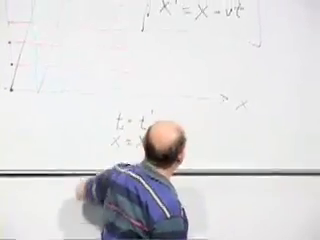
\includegraphics[width=0.72\textwidth]{lecture_01_figure_03.png}
\caption{與兩個時空格架並列表示的伽利略變換。}
\lectureframe{00:21:57}
\end{figure}

第一組方程告訴運動中的觀察者，如何轉換靜止觀察者提供的座標；逆變換則把座標轉回來。這種在兩套描述之間的雙向轉換，就是伽利略相對論的數學內涵。

只有在伽利略理論已經假定\(t=t'\)的前提下，逆向空間公式中的替換\(t\to t'\)才不會造成問題。此處值得留意這個假設。在愛因斯坦的理論中，兩個時間座標會不相同，這類替換也就不再理所當然。

\begin{classroomqa}
\audiencequestion{如果把時鐘帶走再帶回來，我們怎麼知道時鐘的運動沒有先讓它走快、再讓它走慢，以致比較時掩蓋了這種效應？
\lecturetimestamp{00:23:09}}
\lecturerresponse{伽利略不可能以現代的精度確立普遍時間；那只是一個物理上的猜想。我們可以用許多方式檢驗這個猜想：把精確的時鐘朝相反方向帶走，重複往北--南以及往東--西的行程，讓一個時鐘繞著另一個時鐘移動，或不把時鐘帶到一起、改用交換計時訊號的方式比較。在一般速度下，所有這類檢驗的結果都高度一致。時鐘夠精確，或速度夠大時，就會出現微小差異。普遍時間失效並非實驗出了問題；這正是狹義相對論必須解釋的現象之一。}
\end{classroomqa}

\section{伽利略不變量與牛頓定律}

不變量是指所有相關的慣性觀察者都同意的物理量。座標本身不必是不變量。重要的是，由座標寫成的定律是否維持相同形式。

「不變」既可作名詞，也可作形容詞。數值可以是不變量，方程也可以在某種變換下保持不變。區分不變量與不變定律，可以避免一種常見的混淆：相對論並不主張每個觀察者為所有事物測得相同座標；它主張的是，描述各觀察者測量結果之間關係的物理定律，形式相同。

取兩個同時發生、位置分別為\(x_1\)和\(x_2\)的事件。方程~\eqref{eq:galilean-forward}給出
\begin{align}
x_1'&=x_1-vt,\\
x_2'&=x_2-vt.
\end{align}
因此兩事件的間距為
\begin{equation}
x_2'-x_1'=(x_2-vt)-(x_1-vt)=x_2-x_1.
\end{equation}
在伽利略物理學中，同時發生的事件之間的距離是不變量，儘管各事件的位置本身會隨參考系而變。

\begin{classroomqa}
\audiencequestion{這個減法裡的兩個\(t\)，真的是同一個時間嗎？
\lecturetimestamp{00:28:16}}
\lecturerresponse{是的。我們刻意選取了\((x_1,t)\)和\((x_2,t)\)這兩個事件。它們位於同一條水平的等時線上，因此共同項\(vt\)會相消。如果兩個事件發生在不同時間，這個論證就無法證明它們的空間間距是不變量。}
\end{classroomqa}

現在以軌跡\(x(t)\)描述一個粒子。火車上的觀察者會寫成
\begin{equation}
x'(t)=x(t)-vt.
\end{equation}
對兩邊各微分一次，就得到熟悉的速度相加法則：
\begin{equation}
\frac{dx'}{dt}=\frac{dx}{dt}-v.
\end{equation}
位置和速度會隨參考系而變。與箭並行移動的觀察者，會看到箭移動得比站在軌道旁的觀察者慢。

再微分一次。由於相對速度\(v\)是定值，
\begin{equation}
\frac{d^2x'}{dt^2}=\frac{d^2x}{dt^2}.
\end{equation}
加速度在伽利略變換下不變。這有助於理解，為什麼牛頓定律以加速度而非位置或速度表示。

這裡說的是被觀測物體的加速度，而不是火車上觀察者的加速度。兩個參考系都是慣性系，因此彼此之間沒有相對加速度。物體在任一參考系的描述中都可能向左或向右加速；雖然兩位觀察者對物體的位置和速度看法不同，對加速度的數值卻一致。

假設兩個粒子互相施力，而力只取決於它們在同一時刻的間距。這個間距是不變量，因此力也不變。若質量同樣是內在且不依參考系而變的性質，每個慣性觀察者都能用完全相同的形式寫出
\begin{equation}
F=ma
\end{equation}
牛頓力學在伽利略變換下具有不變性。這不只是看來合理；在一般速度的範圍內，牛頓力學極其精確。

這個論證適用於常見的中心力，例如牛頓引力或靜電力；這些力的大小都是距離的函數。所有伽利略觀察者對同一時刻的距離看法一致，因此對力也一致。力和加速度都確定後，為了保持一致，觀察者也必須對質量有相同看法：一個一公斤的物體被火車載著經過時，仍是一個一公斤的物體。\(F=ma\)中的每個符號都符合相同的不變結構。

\section{光不符合伽利略變換規則}

電磁學帶來了難題。麥克斯威方程組預言，波在真空中以確定的速度\(c\)傳播。如果麥克斯威方程組是自然定律，而且自然定律在每個慣性參考系中都相同，那麼所有慣性觀察者測得的\(c\)就必須相同。

伽利略運動學卻預言另一種結果。在靜止參考系中向右傳播的光脈衝滿足
\begin{equation}
x=ct.
\end{equation}
套用空間變換後，得到
\begin{equation}
x'=x-vt=(c-v)t.
\end{equation}
由於\(t'=t\)，火車上的觀察者會測得速度\(c-v\)。

這個矛盾可以明確地表述如下：如果麥克斯威方程組維持原有形式，它們就會預言帶撇號參考系中的速度是\(c\)；如果保留伽利略變換，則會預言速度是\(c-v\)。當\(v\ne0\)時，兩者不可能都完全正確。

如果光像介質中的一般波動，這個結果看起來再自然不過。隨水波移動的船，測得的相對波速會較低；在靜止空氣中移動的聽者，測得的音速也會因聽者相對於空氣的運動而改變。因此，十九世紀的物理學家開始設想有一種優先的靜止狀態，也就是以太參考系；麥克斯威方程組在這個參考系中形式最簡單，光則以\(c\)傳播。為了探測相對於這種優先參考系的運動而設計的實驗，並未發現預期的效應。

實驗可以有好幾種安排，但共同目標都是比較處於不同運動狀態或朝不同方向運動的觀察者所測得的光傳播。沒有任何實驗發現預期的伽利略速度偏移。這次失敗並非小小的技術難題；它迫使人們在相對論原理、麥克斯威方程組，以及沿用已久的空間與時間觀念之間作出抉擇。

愛因斯坦更直接地面對這個衝突。年輕時，他想像自己追逐一列光波。如果他能追上光波，振盪的電磁圖樣就會凝止在空間中；然而麥克斯威方程組不容許這種靜止的光波。他選擇把麥克斯威理論與相對論原理視為基本原則，然後重新檢視座標中隱含的假設。

這套重建以兩條公設為基礎：
\begin{enumerate}
\item 物理定律在每個慣性參考系中都具有相同形式。
\item 真空中的光在每個慣性參考系中都以相同的速度\(c\)傳播。
\end{enumerate}

第二條公設與伽利略變換無法並存。必須改變某種比速度相加法則更深層的東西。愛因斯坦採取了簡潔的作法：保留這兩條公設，重新檢視看似無害的伽利略方程\(t'=t\)。

\section{同步相距遙遠的時鐘}

用尺可以量出空間距離，但要同步相距遙遠的時鐘，還需要一項同步約定。把兩個時鐘放在距離中點觀察者相同的位置。當兩端的時鐘都顯示約定的時刻時，讓它們各自發出一道閃光。如果兩道閃光同時抵達中點，就稱兩端的時鐘已同步。如果其中一道先抵達，就調整相應的時鐘，再重複這項程序。

「\emph{中點}」是根據該參考系中已經標定的尺規來定義的。因此，這項檢驗包含兩個要素：兩端到中點的空間距離相等，以及訊號抵達時間相同。兩者缺一不可。在整個格架上重複這項程序，就能建立牛頓原先直接假定的水平等時線。

這項定義使用光，是因為公設規定光在每個慣性參考系中的速度都相同。如此處理每一對相鄰時鐘後，整個格架就有了一套彼此同步的時鐘。

現在讓第二套格架相對第一套移動。運動裝置的中點在自己的參考系中，仍然位於兩個運動端點的正中間。但相對於靜止裝置，這個中點正朝一束迎面而來的閃光移動，同時遠離另一束閃光。按照靜止時鐘的讀數同時發出的兩道閃光，不會同時抵達運動中的中點。運動中的觀察者採用相同的中點與光訊號方法，因此不會把兩次發射判定為同時。每個參考系都能一致地同步自己的時鐘，但兩套同步方式彼此不同。

這不是因為光傳播需要時間而產生的視覺錯覺。每位觀察者都知道光需要時間才會抵達，也會用相同的速度\(c\)校正這段時間。校正後，分歧仍然存在，因為兩位觀察者選出的同時事件對並不相同。相對的是同時性本身，而不只是同時性的表象。

\begin{classroomqa}
\audiencequestion{如果改用聲音而非光來同步時鐘，能不能避免這個結論？
\lecturetimestamp{00:49:03}}
\lecturerresponse{在空氣靜止的參考系中，聲音可以用來同步時鐘，但它的測得速度並非在每個慣性參考系中都相同。敞篷列車穿過靜止空氣時，列車相對於傳播聲音的介質正在移動，因此向前和向後傳播的聲訊號並不對稱。光依公設則不然：沒有可測出的光學介質，其靜止參考系會選出某個觀察者作為特別對象。因此，我們採用光，並接受由此而來的結果。}
\end{classroomqa}

定性上的差異已經很清楚。現在我們精確計算運動中的觀察者會把哪些事件判定為同時。

\section{光線構造}

為了進行這項構造，採用以下單位會比較方便：
\begin{equation}
c=1.
\end{equation}
如此一來，一個距離單位就是光在一個時間單位內傳播的距離：例如以光秒搭配秒，或以光年搭配年。空間與時間的單位相同，速度沒有量綱，而光線會呈現為\(45^\circ\)。向右傳播的光線滿足
\begin{equation}
x=t+d,
\end{equation}
向左傳播的光線則滿足
\begin{equation}
x=-t+d'.
\end{equation}
通過原點的兩道光線就是\(x=t\)和\(x=-t\)。比光慢的物體所走的類時軌跡，會更靠近垂直軸。假設中的超光速軌跡則會更靠近水平軸。

只有在選定這套單位後，圖中的角度才有意義。如果用公尺和秒，光線看起來幾乎是水平的，因為光在一秒內大約傳播\(3\times10^8\)公尺。以光秒為距離單位，等於重新縮放水平軸，讓因果幾何清楚呈現。

考慮運動格架中的三條平行世界線：
\begin{equation}
x=vt,\qquad x=vt+L,\qquad x=vt+2L.
\label{eq:moving-worldlines}
\end{equation}
中間那條世界線屬於負責檢驗兩個外側格點之間是否同時的觀察者。三個格點都做等速度運動，在帶撇號參考系中彼此的位置關係維持不變。

\begin{figure}[H]
\centering
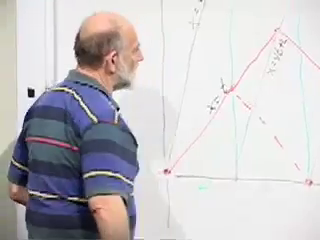
\includegraphics[width=0.72\textwidth]{lecture_01_figure_04.png}
\caption{向右傳播的光線\(x=t\)與中間那條運動世界線的交點。}
\lectureframe{01:02:33}
\end{figure}

完整的幾何構造可以直接畫出來，不必有人站在黑板前擋住畫面：

\begin{figure}[H]
\centering
\begin{tikzpicture}[scale=0.95]
\draw[->] (-0.5,0) -- (6.5,0) node[right] {$x$};
\draw[->] (0,-0.2) -- (0,4.3) node[above] {$t$};
\draw[blue] (0,0) -- (1.4,4.0);
\draw[blue] (2.0,0) -- (3.4,4.0);
\draw[blue] (4.0,0) -- (5.4,4.0);
\draw[red] (0,0) -- (3.08,3.08);
\draw[red] (3.08,3.08) -- (4.56,1.60);
\draw[red,dashed] (2.0,0) -- (4.56,1.60);
\fill (0,0) circle (1.5pt);
\fill (2.0,0) circle (1.5pt);
\fill (4.0,0) circle (1.5pt);
\fill (3.08,3.08) circle (1.5pt);
\fill (4.56,1.60) circle (1.5pt);
\node[left] at (0.55,1.55) {$x=vt$};
\node[left] at (2.45,1.9) {$x=vt+L$};
\node[right] at (4.72,1.9) {$x=vt+2L$};
\node[left] at (1.88,2.28) {$x=t$};
\node[above right] at (3.08,3.08) {$A$};
\end{tikzpicture}
\caption{光訊號決定了運動參考系的等時線。}
\end{figure}

從原點發出一道向右傳播的光線。令\(A\)表示光線與中間世界線的交點。在\(A\)處的兩個方程為
\begin{align}
x&=t,\\
x&=vt+L.
\end{align}
代入後得到
\begin{equation}
t=vt+L,
\end{equation}
因此
\begin{equation}
t_A=x_A=\frac{L}{1-v}.
\label{eq:point-a}
\end{equation}

從\(A\)沿一道向左傳播的光線反向追溯到最右側的運動世界線。這道光線的方程可寫成
\begin{equation}
x+t=b.
\end{equation}
因為光線經過\(A\)，方程~\eqref{eq:point-a}決定了常數：
\begin{equation}
b=x_A+t_A=\frac{2L}{1-v}.
\end{equation}
因此，反向光線滿足
\begin{equation}
x+t=\frac{2L}{1-v}.
\label{eq:backward-ray}
\end{equation}

由下式可求出光線與最右側世界線的交點：
\begin{align}
x+t&=\frac{2L}{1-v},\\
x&=vt+2L.
\end{align}
消去\(x\)後，
\begin{align}
(1+v)t
  &=2L\left(\frac{1}{1-v}-1\right)\\
  &=\frac{2Lv}{1-v},
\end{align}
所以
\begin{equation}
t=\frac{2Lv}{1-v^2}.
\end{equation}
將結果代入\(x=vt+2L\)，得到
\begin{equation}
x=\frac{2L}{1-v^2}.
\end{equation}
座標值本身不如座標之比重要：
\begin{equation}
\frac{t}{x}=v.
\end{equation}
因此，依據運動時鐘的判定，與原點同時的所有事件都位於
\begin{equation}
t=vx,
\label{eq:simultaneity-c-one}
\end{equation}
運動原點則沿著
\begin{equation}
x=vt.
\label{eq:moving-time-axis}
\end{equation}
這兩條軸相對\(45^\circ\)光線呈對稱傾斜。

\(x=vt\)上的所有點都有相同的帶撇號位置\(x'=0\)，但帶撇號時間各不相同。\(t=vx\)上的所有點都有相同的帶撇號時間\(t'=0\)，但帶撇號位置各不相同。因此，一條線是帶撇號時間軸，另一條是帶撇號空間軸。需要透過上述冗長的訊號構造才能確定第二條線；光看運動世界線，無法推知它的位置。

在方程~\eqref{eq:simultaneity-c-one}中恢復一般單位時，需要寫成
\begin{equation}
t=\frac{v}{c^2}x.
\label{eq:simultaneity-dimensional}
\end{equation}
因子\(c^2\)說明了為什麼牛頓的圖像在日常生活中如此適用。速度遠小於\(c\)時，運動參考系的同時線斜率極小。

\begin{figure}[H]
\centering
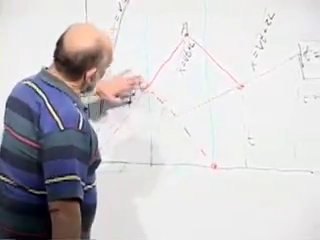
\includegraphics[width=0.72\textwidth]{lecture_01_figure_05.png}
\caption{在\(c=1\)的單位制下，帶撇號時間軸與同時軸以光線為對稱軸。}
\lectureframe{01:15:40}
\end{figure}

\begin{figure}[H]
\centering
\begin{tikzpicture}[scale=1.0]
\draw[->] (-2.2,0) -- (5.2,0) node[right] {$x$};
\draw[->] (0,-0.2) -- (0,4.9) node[above] {$t$};
\draw[red] (0,0) -- (3.9,3.9);
\draw[red] (0,0) -- (-1.8,1.8);
\draw[blue] (0,0) -- (1.8,4.5);
\draw[blue,dashed] (0,0) -- (4.5,1.8);
\node[right] at (3.9,3.9) {$x=t$};
\node[left] at (-1.8,1.8) {$x=-t$};
\node[above] at (1.8,4.5) {$x'=0$};
\node[right] at (4.5,1.8) {$t'=0$};
\end{tikzpicture}
\caption{以\(c=1\)為單位制的帶撇號座標軸與不變光線。}
\end{figure}

\section{推導洛倫茲變換}

幾何構造決定了每個帶撇號座標在哪裡為零。沿著運動時間軸\(x=vt\)，必須有\(x'=0\)；沿著運動同時軸\(t=vx\)，必須有\(t'=0\)。具有這些零值位置的一般線性關係可寫成
\begin{align}
x'&=\frac{x-vt}{F(v)},\\
t'&=\frac{t-vx}{G(v)}.
\label{eq:fg-ansatz}
\end{align}
因子\(F\)和\(G\)允許帶撇號座標的尺度不同於伽利略尺度，即使座標軸的位置已經確定。線性來自空間與時間的均勻性：平移一個實驗，不會改變變換律。\editorialnote{這段簡短的線性論證，明確說明了黑板推導中隱含採用的一項假設。}

到這一步，幾何已經告訴我們許多事情，但還不是全部。分子決定了座標軸的傾斜，卻沒有決定沿著座標軸的單位間距。剩下的尺度資訊正由\(F(v)\)和\(G(v)\)表示。

現在要求光速保持不變。滿足\(x=t\)的向右光線，也必須滿足\(x'=t'\)。沿著這道光線，
\begin{align}
x'&=\frac{(1-v)t}{F(v)},\\
t'&=\frac{(1-v)t}{G(v)}.
\end{align}
要使等式對光線上的每一點都成立，必須有
\begin{equation}
F(v)=G(v).
\end{equation}
因此可以寫成
\begin{align}
x'&=\frac{x-vt}{F(v)},\\
t'&=\frac{t-vx}{F(v)}.
\label{eq:common-f}
\end{align}

這一步在代數推導中首次用到愛因斯坦的關鍵要求。同一條幾何直線對兩位觀察者而言都是光線，因此在\(c=1\)時，沿著這條線變化的兩個帶撇號座標必須等量增加。若兩個方程的因子不同，帶撇號參考系測得的光速就不會是 1。

現在只剩下一個未知函數。將方程~\eqref{eq:common-f}乘以\(F(v)\)：
\begin{align}
F(v)x'&=x-vt,\\
F(v)t'&=t-vx.
\end{align}
將第二式乘以\(v\)，再與第一式相加，便能消去\(t\)，得到
\begin{equation}
(1-v^2)x=F(v)(x'+vt').
\end{equation}
同理，
\begin{equation}
(1-v^2)t=F(v)(t'+vx').
\end{equation}
因此逆變換為
\begin{align}
x&=\frac{F(v)}{1-v^2}(x'+vt'),\\
t&=\frac{F(v)}{1-v^2}(t'+vx').
\end{align}

相對論原理要求兩個參考系彼此對等。如果車站觀察到火車以\(+v\)移動，火車就會觀察到車站以\(-v\)移動。因此，逆變換方程的形式必須與正變換相同，只把\(v\)的符號反轉。兩式的前置因子必須滿足
\begin{equation}
\frac{F(v)}{1-v^2}=\frac{1}{F(v)}.
\end{equation}
因此
\begin{equation}
F(v)^2=1-v^2,
\end{equation}
再根據\(v=0\)時變換須連續地回到恆等變換，選取正根：
\begin{equation}
F(v)=\sqrt{1-v^2}.
\end{equation}

這個結果不是根據某一道特定的光脈衝調整而得。它來自同步程序所確定的座標軸、共同的光速，以及兩個慣性參考系都不應享有優先地位的要求。

在\(c=1\)的單位制下，洛倫茲變換為
\begin{align}
x'&=\frac{x-vt}{\sqrt{1-v^2}},\\
t'&=\frac{t-vx}{\sqrt{1-v^2}}.
\label{eq:lorentz-c-one}
\end{align}
其逆變換為
\begin{align}
x&=\frac{x'+vt'}{\sqrt{1-v^2}},\\
t&=\frac{t'+vx'}{\sqrt{1-v^2}}.
\end{align}

\begin{figure}[H]
\centering
\includegraphics[width=0.76\textwidth]{lecture_01_figure_06.png}
\caption{黑板上完成的\(c=1\)洛倫茲變換。}
\lectureframe{01:32:38}
\end{figure}

關鍵的新意已經出現在時間方程中。時間不會從一個參考系原封不動地轉換到另一個參考系；帶撇號的時間座標混合了原本的時間與位置。因此，\(t=\text{constant}\)和\(t'=\text{constant}\)描述的是不同的事件集合。

混合項不是事後添加的可有可無的修正。少了它，直線\(t'=0\)就會維持水平，遠處事件的同時性也會是普遍不變的，而變換便無法保持光速不變。

\section{恢復光速並檢驗結果}

當\(c\ne1\)時，為了符合量綱，必須補回缺少的因子。比值\(v^2/c^2\)沒有量綱，而\((v/c^2)x\)的量綱是時間。因此
\begin{align}
x'&=\frac{x-vt}{\sqrt{1-v^2/c^2}},\\
t'&=\frac{t-(v/c^2)x}{\sqrt{1-v^2/c^2}}.
\label{eq:lorentz-dimensional}
\end{align}
將\(v\)的符號反轉，即得逆變換：
\begin{align}
x&=\frac{x'+vt'}{\sqrt{1-v^2/c^2}},\\
t&=\frac{t'+(v/c^2)x'}{\sqrt{1-v^2/c^2}}.
\end{align}
引入
\begin{equation}
\gamma=\frac{1}{\sqrt{1-v^2/c^2}}
\end{equation}
即可寫成常見的簡潔形式；不過，使用分母的寫法能讓推導過程一目了然。

數值上，\(c\simeq3\times10^8\,\mathrm{m/s}\)，所以\(c^2\simeq9\times10^{16}\,\mathrm{m^2/s^2}\)。分母很大，因此在大多數力學實驗中，同時線的傾斜和因子\(v^2/c^2\)都難以察覺。這些效應很小，說明了伽利略理論為何如此成功；但它們並未使絕對時間重獲成立。

\begin{figure}[H]
\centering
\includegraphics[width=0.76\textwidth]{lecture_01_figure_07.png}
\caption{補回\(c\)因子後的洛倫茲變換。}
\lectureframe{01:35:58}
\end{figure}

有兩項檢驗可以立即進行。首先，令\(v\ll c\)。此時\(v^2/c^2\)可忽略；對一般距離而言，同時性的相對性項\(vx/c^2\)也可忽略。式~\eqref{eq:lorentz-dimensional}便化為
\begin{equation}
t'\approx t,\qquad x'\approx x-vt.
\end{equation}
在低速近似下，便可恢復伽利略相對性。

其次，檢驗一條光線。把\(c\)放回方程式後，向右行進的光線滿足\(x=ct\)，而非\(x=t\)。代入後得到
\begin{align}
x'&=\frac{(c-v)t}{\sqrt{1-v^2/c^2}},\\
t'&=\frac{(1-v/c)t}{\sqrt{1-v^2/c^2}}.
\end{align}
由於\(c-v=c(1-v/c)\)，
\begin{equation}
x'=ct'.
\end{equation}
帶撇號參考系中的觀察者測得的光速仍是\(c\)。對向左行進的光線，代入\(x=-ct\)也同樣得到
\begin{equation}
x'=-ct'.
\end{equation}
這個變換能正確描述兩個方向上的光。

\(x=t\)與\(x=ct\)的區別，是一項有助於檢查量綱的例子。前者只有在\(c=1\)的單位制下才正確。若在變換中恢復通常單位，卻仍以自然單位表示光線方程式，就會混用兩種約定，導致錯誤結果。量綱一致性檢查能立即發現這個錯誤。

\section{中點判準}

\begin{classroomqa}
\audiencequestion{假設一位觀察者同時接收到兩道閃光，但他不在兩個光源的中點。這位觀察者能否據此斷定兩道閃光是同時發出的？
\lecturetimestamp{01:42:55}}
\lecturerresponse{不能。只有對於在相關參考系中位於兩個光源空間中點的觀察者，到達時間相同才表示發射時間相同。較靠近其中一個光源的接收者，可能同時收到兩道閃光，即使較遠處的那道閃光發射得更早。在運動構造中，中點世界線\(x=vt+L\)因此不可或缺。沿著向前的光線\(x=t\)追蹤，直到它與該中點相交；接著沿反向的光線追到\(x=vt+2L\)。按照運動參考系的判定，這第二個端點事件才與原點同時，而不是其他位置任意一個到達時間相同的事件。}
\end{classroomqa}

我們已得到完整的座標變換，但它最熟悉的推論還有待導出。接下來將討論長度收縮、時間膨脹與固有時間，然後是相對論動量和能量。基礎已經具備：空間與時間會彼此混合，因此每個慣性系才能使用相同的定律並測得相同的光速；遠距同時性則取決於參考系，並非世界本身具有的絕對性。
\chapter{麥克斯威方程、協變性與電磁波}

\lectureoverview{電場和磁場透過洛倫茲力作用於帶電物質，但物質也會產生並重新分布場。我們將探討電磁學中物質對場作用的這一面，說明麥克斯威方程具有洛倫茲協變性，推導其波動解，最後以能明確呈現局域守恆的形式重新納入電荷和電流。整堂課都採用\(c=1\)的單位制。}

\section{電磁學的另一面}

先從已經學過的部分開始。若一個電荷為\(q\)的粒子以速度\(\mathbf v\)穿越電場和磁場，所受的力為
\begin{equation}
\mathbf F=q\bigl(\mathbf E+\mathbf v\times\mathbf B\bigr).
\label{eq:lorentz-force-three}
\end{equation}
因子\(q\)不可或缺。中性粒子不會受到電磁力。即使粒子瞬間靜止，電場仍會產生作用；磁場的作用則取決於粒子的運動。

方程~\eqref{eq:lorentz-force-three}告訴我們給定的場如何作用於物質，卻沒有說明場是由什麼決定的。是什麼在某個物體周圍產生電場、在另一個物體周圍產生磁場，或在真空中產生傳播的波？回答這些問題的就是麥克斯威方程。

\begin{figure}[H]
\centering
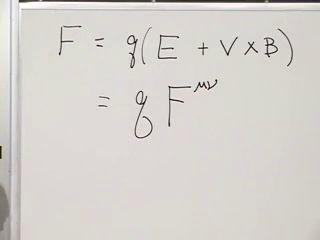
\includegraphics[width=0.62\textwidth]{lecture_58_figure_02.png}
\caption{三維向量形式的洛倫茲力，以及將其改寫為張量形式的開端。}
\lectureframe{00:05:49}
\end{figure}

力定律的相對論形式預示了接下來要用的記號：
\begin{equation}
f^\mu=qF^\mu{}_{\nu}u^\nu.
\label{eq:lorentz-force-four}
\end{equation}
其中，\(u^\nu\)是四速度，\(f^\mu\)是四力，而\(F^{\mu\nu}\)是由\(\mathbf E\)和\(\mathbf B\)組成的反對稱張量。黑板上先只寫出這個表示式的示意性開頭；與\(u^\nu\)縮並後，才會得到留下單一自由力指標所需的向量。

物質必須反過來作用於場，這有其物理理由。電磁波可以撞上電荷，使它加速，並將能量傳給它。如果場能影響電荷，而電荷卻永遠不能影響場，那麼場傳給電荷的能量就無從而來。作用與反作用還不足以說明全部，但能量守恆使這種相互耦合不可避免。

\section{變動的源會發出擾動}

點電荷會產生一個從其位置向外或向內指向的電場。導線中的電流--也就是帶電粒子的流動--則會產生環繞導線的磁場。這些熟悉的靜態圖像已呈現兩種不同的幾何形態：電通量由電荷向外發出，磁力線則環繞電流。

現在讓點電荷突然移動。在它的新位置附近，電場必須開始重新分布；但遠方的觀察者不可能立即得知它已移動。在訊號抵達之前，遠方的舊場仍維持原狀。近處與遠處之間有一道移動的前沿，場在此處發生變化。這道移動中的場變化就是電磁擾動。

若電荷來回振盪，連續的場變化便接踵而至，形成電磁波。這就是天線的基本作用：振盪電流向外發出場的擾動。將導線中的電流反向，也可用同樣的論證說明磁場的情形。\(\mathbf B\)的環流必須反向，但這個變化會向外傳播，不會同時出現在各處。

這個因果圖像為麥克斯威方程設定了兩個目標：描述電荷和電流如何作為場的源，並允許場的變化以不超過光速的速度傳播。第二個目標也可用來檢驗相對論。如果麥克斯威方程在每個慣性參考系中形式相同，且蘊含一個確定的波速，那麼每個慣性參考系都必須從中推得相同的速度。

\section{回顧相對論波動方程}

在討論向量場之前，先考慮標量場\(\phi(\mathbf x,t)\)，也就是時空中每一點都有一個數值的場。一個一階導數方程
\begin{equation}
\partial_\mu\phi=0
\end{equation}
表示所有時空方向的導數都為零。這樣的場會是常數，因此無法承載波。非平凡的相對論波動方程需要二階導數：
\begin{equation}
\partial_\mu\partial^\mu\phi=0.
\end{equation}
按照這裡採用的符號慣例，
\begin{equation}
\left(\partial_t^2-\partial_x^2-\partial_y^2-\partial_z^2\right)\phi=0,
\label{eq:scalar-wave-four}
\end{equation}
也可以更精簡地寫成
\begin{equation}
\left(\partial_t^2-\nabla^2\right)\phi=0.
\end{equation}
採用\(c=1\)，可使時間和距離使用相容的單位。恢復一般單位制時，二階時間導數前會出現\(1/c^2\)。

若波沿\(z\)軸傳播，場只依賴\(z\)和\(t\)，不依賴\(x\)或\(y\)。方程~\eqref{eq:scalar-wave-four}便化為
\begin{equation}
\left(\partial_t^2-\partial_z^2\right)\phi=0.
\label{eq:scalar-wave-one}
\end{equation}

\begin{figure}[H]
\centering
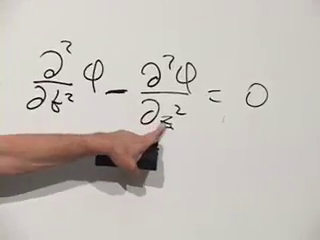
\includegraphics[width=0.56\textwidth]{lecture_58_figure_04.png}
\caption{作為電磁波模型的一維標量波動方程。}
\lectureframe{00:47:03}
\end{figure}

其一般行波解為
\begin{equation}
\phi(z,t)=f(z-t)+g(z+t).
\end{equation}
波形\(f(z-t)\)沿\(z\)增大的方向傳播，因為相位固定的點滿足\(z-t=\text{constant}\)。波形\(g(z+t)\)則朝相反方向傳播。兩個波形都不必是正弦波；只要形狀足夠平滑，就能在平移時維持原形。

不過，正弦波很方便使用：
\begin{equation}
\phi(z,t)=A\cos\!\bigl(k(z-t)\bigr).
\end{equation}
波數\(k\)決定波長，
\begin{equation}
\lambda=\frac{2\pi}{k}.
\end{equation}
\(k\)較大時，空間振盪較快、波長較短；\(k\)較小時，波長較長。這些波形很快就會成為\(\mathbf E\)和\(\mathbf B\)的分量。

\section{麥克斯威方程所需的向量微積分}

麥克斯威方程以點積、叉積、散度和旋度表示。值得先重新整理一次這些記號，因為後續的分量計算會用到這些運算形式。

對一般三維向量\(\mathbf a\)和\(\mathbf b\)而言，點積是純量：
\begin{equation}
\mathbf a\cdot\mathbf b
=a_xb_x+a_yb_y+a_zb_z.
\end{equation}
叉積則是另一個向量：
\begin{align}
(\mathbf a\times\mathbf b)_x&=a_yb_z-a_zb_y,\\
(\mathbf a\times\mathbf b)_y&=a_zb_x-a_xb_z,\\
(\mathbf a\times\mathbf b)_z&=a_xb_y-a_yb_x.
\end{align}
其餘分量可依循環順序\(x\to y\to z\to x\)得到。

引入微分算子
\begin{equation}
\boldsymbol\nabla=
\left(\partial_x,\partial_y,\partial_z\right).
\end{equation}
它的分量是算子而非一般數值，但仍可依照點積和叉積的運算形式計算。對向量場\(\mathbf A\)而言，
\begin{equation}
\boldsymbol\nabla\cdot\mathbf A
=\partial_xA_x+\partial_yA_y+\partial_zA_z
\label{eq:divergence}
\end{equation}
是散度；
\begin{align}
(\boldsymbol\nabla\times\mathbf A)_x
 &=\partial_yA_z-\partial_zA_y,\\
(\boldsymbol\nabla\times\mathbf A)_y
 &=\partial_zA_x-\partial_xA_z,\\
(\boldsymbol\nabla\times\mathbf A)_z
 &=\partial_xA_y-\partial_yA_x
\label{eq:curl}
\end{align}
則是旋度的各分量。

幾何圖像和公式同樣重要。向量場看起來由某處向外流出時，該處的散度為正；場呈環流狀時，則有旋度。點電荷的徑向電場可說明散度，載流導線周圍環繞的磁場則可說明旋度。空間中均勻的向量場兩者皆無。

\section{真空中的麥克斯威方程}

沒有電荷和電流時，麥克斯威方程為
\begin{align}
\boldsymbol\nabla\times\mathbf E&=-\partial_t\mathbf B,
\label{eq:faraday-vac}\\
\boldsymbol\nabla\cdot\mathbf B&=0,
\label{eq:gauss-b-vac}\\
\boldsymbol\nabla\times\mathbf B&=\partial_t\mathbf E,
\label{eq:ampere-vac}\\
\boldsymbol\nabla\cdot\mathbf E&=0.
\label{eq:gauss-e-vac}
\end{align}
兩個旋度方程幾乎可以互換\(\mathbf E\)與\(\mathbf B\)，但關鍵的負號使兩者有所不同。兩個散度方程則表示，在所考慮的真空區域內，兩個場都沒有源。即使重新納入電荷源，磁場的散度仍為零；一般電磁學不包含磁荷。

\begin{figure}[H]
\centering
\includegraphics[width=0.76\textwidth]{lecture_58_figure_06.png}
\caption{四個真空中的麥克斯威方程，排列方式呈現電場與磁場之間近似的對稱性。}
\lectureframe{00:27:30}
\end{figure}

最後，電荷密度\(\rho\)會取代方程~\eqref{eq:gauss-e-vac}右側的零，而電流密度\(\mathbf J\)會出現在方程~\eqref{eq:ampere-vac}中。這些項目暫且先不納入。無源方程的形式較簡潔，能清楚呈現變換結構和波的形成機制。

它們也讓愛因斯坦的難題更加尖銳。若以伽利略變換描述一位隨波移動的觀察者，他會預期速度相減，測得較小的波速。然而，若麥克斯威方程在每個慣性參考系中都成立，每位觀察者就都會推得相同的單位波速。解決之道不是在不同參考系中改變波動方程，而是使用洛倫茲變換，並以變換律已知的物件來表示麥克斯威方程。

\section{電場與磁場組成同一個張量}

電場和磁場組合成反對稱的場張量
\begin{equation}
F^{\mu\nu}=
\begin{pmatrix}
0   & -E_x & -E_y & -E_z\\
E_x & 0    & -B_z & B_y\\
E_y & B_z  & 0    & -B_x\\
E_z & -B_y & B_x  & 0
\end{pmatrix},
\label{eq:l0203-field-tensor}
\end{equation}
矩陣的列與行依\(t,x,y,z\)排列。反對稱性
\begin{equation}
F^{\mu\nu}=-F^{\nu\mu},
\end{equation}
使對角元素必為零，也決定了矩陣下半部的元素由上半部給出。時間與空間方向交錯的元素包含\(\mathbf E\)；純空間方向的元素則包含\(\mathbf B\)。

\begin{figure}[H]
\centering
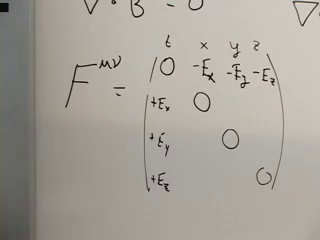
\includegraphics[width=0.58\textwidth]{lecture_58_figure_03.png}
\caption{完整的電磁場張量，包含電場與磁場的元素。}
\lectureframe{00:32:05}
\end{figure}

\(F^{\mu\nu}\)的重要性不只在於能將六個場分量收納在同一個矩陣中。在洛倫茲變換下，它依照二階張量的變換律變換。因此，不同觀察者測得的電場和磁場會恰當地混合，使整個張量能一致地變換。

還有另一個反對稱張量，稱為對偶場張量\(\widetilde F^{\mu\nu}\)。依照目前採用的慣例，從方程~\eqref{eq:l0203-field-tensor}出發，以如下替換
\begin{equation}
\mathbf E\longmapsto-\mathbf B,
\qquad
\mathbf B\longmapsto\mathbf E.
\label{eq:dual-replacement}
\end{equation}
便可得到對偶張量：
\begin{equation}
\widetilde F^{\mu\nu}=
\begin{pmatrix}
0    & B_x  & B_y  & B_z\\
-B_x & 0    & -E_z & E_y\\
-B_y & E_z  & 0    & -E_x\\
-B_z & -E_y & E_x  & 0
\end{pmatrix}.
\label{eq:dual-tensor}
\end{equation}
方程~\eqref{eq:dual-replacement}中的符號至關重要。講課時先口頭交換電場與磁場，隨即發現符號不符，於是先修正符號，再完成矩陣。

\begin{figure}[H]
\centering
\includegraphics[width=0.58\textwidth]{lecture_58_figure_07.png}
\caption{以必要的符號交換電場與磁場元素，組成對偶張量。}
\lectureframe{00:35:45}
\end{figure}

\section{協變形式的真空方程}

每個麥克斯威方程都含有一個導數。從二階張量出發，將一個指標與導數縮並後，會留下一個自由指標，因此自然的協變形式候選式為
\begin{align}
\partial_\mu F^{\mu\nu}&=0,
\label{eq:maxwell-covariant-vac}\\
\partial_\mu\widetilde F^{\mu\nu}&=0.
\label{eq:maxwell-dual-vac}
\end{align}
固定\(\nu\)後，方程~\eqref{eq:maxwell-covariant-vac}就是一條方程。由於\(\nu\)可以取\(t,x,y,z\)，這個式子涵蓋四條純量方程。方程~\eqref{eq:maxwell-dual-vac}則涵蓋另外四條。這正好對應原先列出的兩個向量旋度方程和兩個純量散度方程。

緊湊的記號必須能重現熟悉的方程才有用。取\(\nu=z\)：
\begin{align}
\partial_\mu F^{\mu z}
&=\partial_tF^{tz}
  +\partial_xF^{xz}
  +\partial_yF^{yz}
  +\partial_zF^{zz}\\
&=-\partial_tE_z+\partial_xB_y-\partial_yB_x\\
&=-\partial_tE_z+
  \bigl(\boldsymbol\nabla\times\mathbf B\bigr)_z.
\end{align}
項\(F^{zz}\)因反對稱性而消失。令結果等於零，就得到
\(z\)分量的方程：
\begin{equation}
\boldsymbol\nabla\times\mathbf B=\partial_t\mathbf E.
\end{equation}
\(x\)和\(y\)分量則可循環更換指標得到。

\begin{figure}[H]
\centering
\includegraphics[width=0.76\textwidth]{lecture_58_figure_08.png}
\caption{協變場方程的分量展開：對角張量元素為零，其餘項則還原出麥克斯威方程。}
\lectureframe{00:43:30}
\end{figure}

接著取時間分量：
\begin{align}
\partial_\mu F^{\mu t}
&=\partial_tF^{tt}
  +\partial_xF^{xt}
  +\partial_yF^{yt}
  +\partial_zF^{zt}\\
&=\partial_xE_x+\partial_yE_y+\partial_zE_z\\
&=\boldsymbol\nabla\cdot\mathbf E.
\end{align}
這便得到方程~\eqref{eq:gauss-e-vac}。對偶張量也可用同樣方式檢查，得到
\(\boldsymbol\nabla\cdot\mathbf B=0\)以及
\(\boldsymbol\nabla\times\mathbf E=-\partial_t\mathbf B\)。

現在已經推導出這些緊湊方程，而非僅僅猜測它們。自由指標的結構使它們成為四向量方程，因此洛倫茲變換會改變方程的分量，卻不改變其形式。這就是真空中的麥克斯威方程在每個慣性參考系中形式相同的確切意義。

\section{從一階方程推得波動方程}

麥克斯威方程只含一階導數，而波動方程含有二階導數。這看似不一致，但麥克斯威理論耦合了兩個場，因此可以將\(\mathbf E\)和\(\mathbf B\)的一對一階方程合併，得到任一場各自滿足的二階方程。

將方程~\eqref{eq:ampere-vac}對時間微分：
\begin{equation}
\partial_t^2\mathbf E
=\boldsymbol\nabla\times\partial_t\mathbf B.
\end{equation}
法拉第定律給出\(\mathbf B\)的時間導數：
\begin{equation}
\partial_t\mathbf B=-\boldsymbol\nabla\times\mathbf E,
\end{equation}
因此
\begin{equation}
\partial_t^2\mathbf E
=-\boldsymbol\nabla\times
  \bigl(\boldsymbol\nabla\times\mathbf E\bigr).
\label{eq:double-curl}
\end{equation}

黑板上的推導逐一計算各分量，並未直接引用熟記的恆等式。以\(x\)分量為例：
\begin{align}
\bigl[\boldsymbol\nabla\times
(\boldsymbol\nabla\times\mathbf E)\bigr]_x
&=\partial_y(\boldsymbol\nabla\times\mathbf E)_z
 -\partial_z(\boldsymbol\nabla\times\mathbf E)_y\\
&=\partial_y(\partial_xE_y-\partial_yE_x)\\
&\quad-\partial_z(\partial_zE_x-\partial_xE_z)\\
&=\partial_x(\partial_yE_y+\partial_zE_z)
 -\partial_y^2E_x\\
&\quad-\partial_z^2E_x.
\end{align}
加上再減去\(\partial_x^2E_x\)，即可整理出散度：
\begin{align}
\bigl[\boldsymbol\nabla\times
(\boldsymbol\nabla\times\mathbf E)\bigr]_x
&=\partial_x(\boldsymbol\nabla\cdot\mathbf E)
 -\nabla^2E_x.
\label{eq:double-curl-x}
\end{align}
在真空中，\(\boldsymbol\nabla\cdot\mathbf E=0\)。合併方程~\eqref{eq:double-curl}與\eqref{eq:double-curl-x}，得到
\begin{equation}
\left(\partial_t^2-\nabla^2\right)E_x=0.
\label{eq:ex-wave}
\end{equation}

\begin{figure}[H]
\centering
\includegraphics[width=0.72\textwidth]{lecture_58_figure_09.png}
\caption{逐分量計算後，得到\(E_x\)的波動方程。}
\lectureframe{00:57:10}
\end{figure}

同樣的計算也適用於\(E_y\)和\(E_z\)，以類似方式消去另一個場後可得
\begin{equation}
\left(\partial_t^2-\nabla^2\right)\mathbf B=0.
\end{equation}
因此，電場和磁場都能以波的形式在真空中傳播。採用這裡的單位制時，波速為一；恢復一般單位後，波速就是\(c\)。

\section{平面波與偏振}

考慮一個沿\(z\)正方向傳播的簡單波：
\begin{equation}
\mathbf E(z,t)
=\widehat{\mathbf x}\,E_0
  \cos\!\bigl(k(z-t)\bigr).
\label{eq:plane-e}
\end{equation}
波形沿\(z\)方向平移而不改變形狀。由於電場沿\(x\)軸，這個波在\(x\)方向上呈線偏振。我們選擇\(E_y=0\)只是為了簡化例子；也可以加入第二種橫向偏振。

縱向分量則不能任意變化。由於波只依賴\(z\)和\(t\)，
\begin{equation}
\boldsymbol\nabla\cdot\mathbf E
=\partial_zE_z=0.
\end{equation}
所以\(E_z\)可以是常數，卻不能包含隨波變化的部分。均勻背景場可以獨立地疊加或移除，但它不屬於傳播中的輻射。波本身是橫向的：
\begin{equation}
\mathbf E_{\mathrm{wave}}\cdot\widehat{\mathbf z}=0.
\end{equation}

法拉第定律決定了磁場。對於方程~\eqref{eq:plane-e}，\(\boldsymbol\nabla\times\mathbf E\)只有\(y\)分量不為零：
\begin{equation}
(\boldsymbol\nabla\times\mathbf E)_y=\partial_zE_x.
\end{equation}
因此\(\partial_t\mathbf B\)沿\(y\)方向；一個符合條件的選擇是
\begin{equation}
\mathbf B(z,t)
=\widehat{\mathbf y}\,E_0
  \cos\!\bigl(k(z-t)\bigr).
\label{eq:plane-b}
\end{equation}
在這個單位制下，電場和磁場的振幅相等。兩者的方向關係為
\begin{equation}
\mathbf E\perp\mathbf B,
\qquad
\mathbf E\perp\widehat{\mathbf z},
\qquad
\mathbf B\perp\widehat{\mathbf z},
\qquad
\mathbf E\times\mathbf B\parallel\widehat{\mathbf z}.
\end{equation}

\begin{figure}[H]
\centering
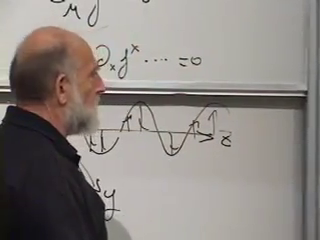
\includegraphics[width=0.70\textwidth]{lecture_58_figure_05.png}
\caption{完整的黑板示意圖呈現橫電磁波：電場和磁場的振盪彼此垂直，且都垂直於傳播方向。}
\lectureframe{01:05:25}
\end{figure}

\begin{figure}[H]
\centering
\scalebox{0.90}{%
\begin{tikzpicture}[x=1cm,y=1cm,>=Latex]
  \draw[->,thick] (0,0) -- (8.2,0) node[right] {$z$};
  \draw[->,thick] (0,-1.6) -- (0,1.7) node[above] {$x$};
  \draw[->,thick] (0,0) -- (-1.15,-0.8) node[below left] {$y$};
  \draw[blue!70!black,thick,domain=0:7.5,samples=120]
    plot (\x,{0.95*sin(90*\x)});
  \foreach \z/\s in {0.8/1,2.8/-1,4.8/1,6.8/-1}{
    \draw[->,green!45!black,thick]
      (\z,0) -- ++({-0.55*\s},{-0.38*\s});
  }
  \node[blue!70!black] at (6.9,1.25) {$\mathbf E$};
  \node[green!45!black] at (5.2,-1.05) {$\mathbf B$};
  \draw[->,very thick] (6.2,1.55) -- (7.7,1.55)
    node[midway,above] {propagation};
\end{tikzpicture}
}
\caption{場\(\mathbf E\)和\(\mathbf B\)彼此垂直，且都垂直於傳播方向。}
\end{figure}

這就是光以及所有真空中電磁輻射的特性。由於導出此波的方程具有洛倫茲協變性，另一位慣性觀察者也會描述一個以\(c\)傳播、具有橫向電場和磁場的電磁波。

\section{電荷密度與電流密度}

現在重新納入先前暫時擱置的源。當許多帶電粒子分布在一個區域內時，可將其粗粒化，並以連續的電荷密度描述：
\begin{equation}
\rho(\mathbf x,t)=\frac{dQ}{dV}.
\end{equation}
這種近似就像將水視為連續流體，儘管水是由分子組成。正電荷和負電荷的貢獻符號相反，因此\(\rho\)代表每單位體積的淨電荷。

選定區域\(V\)內的電荷為
\begin{equation}
Q_V(t)=\int_V\rho(\mathbf x,t)\,dV.
\label{eq:charge-volume}
\end{equation}
電荷密度可以隨位置和時間變化。一團電荷移離某點時，該處的局域密度便會改變。但電荷密度不能任意變化，因為電荷守恆。

只要求總量守恆還不夠。這會容許電荷在同一瞬間從地球消失、又在火星出現，只要總量不變即可。更強的局域守恆敘述是：電荷只能經由中間空間中的流動，從一處離開並抵達另一處。

為描述這種流動，取一個無窮小的有向面積元素
\begin{equation}
d\boldsymbol\sigma=\widehat{\mathbf n}\,d\sigma.
\end{equation}
其大小為面積，方向則垂直於表面。電流密度\(\mathbf J\)的定義是：單位時間內穿過此面積元素的電荷量為
\begin{equation}
\frac{dQ}{dt}=\mathbf J\cdot d\boldsymbol\sigma.
\label{eq:current-flux-element}
\end{equation}
\(\mathbf J\)的大小表示單位面積、單位時間內通過的電荷量，方向則與正電荷流動方向一致。

\begin{figure}[H]
\centering
\includegraphics[width=0.64\textwidth]{lecture_58_figure_10.png}
\caption{有向面積元素與通量因子\(d\boldsymbol\sigma\cdot\mathbf J\)。}
\lectureframe{01:18:15}
\end{figure}

點積會選出垂直於表面的分量。沿表面切向流動的電流不會穿過表面的任一側，因此通量為零。若電流平行於法線，在電流大小固定時，通量最大。導線中的電流只是其中一種情況；\(\mathbf J\)也可以描述電荷流經薄片，或在整個三維空間中流動。

\section{局域守恆與連續方程}

固定空間中的區域\(V\)，並使其封閉邊界\(\partial V\)上的每個面積元素都朝外取向。若有淨電流向外流出，區域內的電荷量便會減少：
\begin{equation}
\frac{dQ_V}{dt}
=-\oint_{\partial V}\mathbf J\cdot d\boldsymbol\sigma.
\label{eq:integral-conservation}
\end{equation}
這個負號反映的是物理意義，而非記號慣例：向外的正通量會帶走區域內的正電荷。利用方程~\eqref{eq:charge-volume}，可得
\begin{equation}
\int_V\partial_t\rho\,dV
=-\oint_{\partial V}\mathbf J\cdot d\boldsymbol\sigma.
\label{eq:integral-continuity-one}
\end{equation}

\begin{figure}[H]
\centering
\includegraphics[width=0.72\textwidth]{lecture_58_figure_11.png}
\caption{將表面通量轉寫為體積積分後，固定區域的守恆定律。}
\lectureframe{01:29:00}
\end{figure}

高斯定理，也稱為散度定理，將穿過封閉曲面的通量與曲面內部的散度連結起來：
\begin{equation}
\oint_{\partial V}\mathbf A\cdot d\boldsymbol\sigma
=\int_V\boldsymbol\nabla\cdot\mathbf A\,dV.
\label{eq:divergence-theorem}
\end{equation}
可以想像容器內有看不見的管道，在內部各處注入水。散度衡量水從管道出口流出的局域速率；曲面積分則衡量離開容器的水量總和。容器內部產生的向外流動，最終都必須穿過邊界。

將方程~\eqref{eq:divergence-theorem}應用於\(\mathbf J\)，得到
\begin{equation}
\int_V
\left(\partial_t\rho+\boldsymbol\nabla\cdot\mathbf J\right)dV=0.
\end{equation}
此關係對每一個可能的區域\(V\)都成立。因此，被積函數必須在每一點都為零：
\begin{equation}
\boxed{\partial_t\rho+\boldsymbol\nabla\cdot\mathbf J=0.}
\label{eq:continuity-three}
\end{equation}

\begin{figure}[H]
\centering
\includegraphics[width=0.72\textwidth]{lecture_58_figure_12.png}
\caption{以分量形式表示的局域連續方程。}
\lectureframe{01:29:50}
\end{figure}

方程~\eqref{eq:continuity-three}正是局域守恆所要求的條件。如果某點或某個小區域內的電荷密度減少，電流就必須從該處向外發散；如果電流向內匯聚，電荷密度便會增加。

電荷密度與電流自然地組成四電流
\begin{equation}
J^\mu=(\rho,J_x,J_y,J_z)
\label{eq:four-current}
\end{equation}
單位制採用\(c=1\)時，連續方程可寫成洛倫茲純量方程
\begin{equation}
\partial_\mu J^\mu=0.
\label{eq:continuity-four}
\end{equation}
相對論性分布的流量應像單一粒子的四速度一樣，依四向量的變換律變換。方程~\eqref{eq:continuity-four}確保局域電荷守恆在每個慣性參考系中都成立。

\section{有源麥克斯威方程}

重新納入電荷和電流後，得到
\begin{align}
\boldsymbol\nabla\cdot\mathbf E&=\rho,
\label{eq:gauss-e-source}\\
\boldsymbol\nabla\cdot\mathbf B&=0,\\
\boldsymbol\nabla\times\mathbf E&=-\partial_t\mathbf B,\\
\boldsymbol\nabla\times\mathbf B&=\partial_t\mathbf E+\mathbf J.
\label{eq:ampere-source}
\end{align}
涉及電場源的方程可合併為
\begin{equation}
\boxed{\partial_\mu F^{\mu\nu}=J^\nu,}
\label{eq:maxwell-source-covariant}
\end{equation}
而磁場的無源方程仍為
\begin{equation}
\boxed{\partial_\mu\widetilde F^{\mu\nu}=0.}
\label{eq:maxwell-dual-source}
\end{equation}

\begin{figure}[H]
\centering
\includegraphics[width=0.78\textwidth]{lecture_58_figure_13.png}
\caption{含源項的麥克斯威方程及其協變形式\(\partial_\mu F^{\mu\nu}=J^\nu\)。}
\lectureframe{01:34:00}
\end{figure}

方程~\eqref{eq:maxwell-source-covariant}的時間分量為
\begin{equation}
\partial_\mu F^{\mu t}=J^t=\rho,
\end{equation}
前面已完成的分量計算可將其左側化為
\(\boldsymbol\nabla\cdot\mathbf E\)。三個空間分量則還原出
\(\boldsymbol\nabla\times\mathbf B=\partial_t\mathbf E+\mathbf J\)。

還可以做一個有用的一致性檢查。對方程~\eqref{eq:maxwell-source-covariant}作用\(\partial_\nu\)，得到
\begin{equation}
\partial_\nu J^\nu
=\partial_\nu\partial_\mu F^{\mu\nu}=0,
\end{equation}
這是因為兩個導數在\(\mu\leftrightarrow\nu\)交換下對稱，而\(F^{\mu\nu}\)是反對稱的。\editorialnote{這個簡短的一致性檢查直接來自協變方程，並清楚說明為何含源項的麥克斯威方程會自動滿足連續方程。}

至此，相互作用的結構已完整建立。張量形式的力定律
\(f^\mu=qF^\mu{}_\nu u^\nu\)描述場如何作用於電荷，而方程~\eqref{eq:maxwell-source-covariant}則描述電荷與電流如何產生場。兩者都是張量方程。在真空中，同一組場方程會導出以\(c\)傳播的橫波。因此，洛倫茲協變性與電磁波方程在最初促使我們進行這項推導之處交會：每位慣性觀察者都會得到相同的電磁定律和相同的光速。
\chapter{固有時、時間膨脹與長度收縮}

我們經常選用光速為$c=1$的單位制。在這種單位制下，一年的時間與一光年的距離可以直接比較，公式也更容易閱讀。只要$c$在物理上不可忽略，我們就會把它放回公式中。量綱分析足以判定它應放在何處。

\section{伽利略時空網格}

先從愛因斯坦之前描述靜止參考系與沿$x$軸以速度$v$運動的列車之間關係的公式開始：
\begin{align}
x' &= x-vt, & t'&=t.
\label{eq:l4-galilean}
\end{align}
第二個方程包含了牛頓對普適時間的假設。即使空間原點彼此相對運動，每位觀測者使用的同時性切片仍然相同。

假設不帶撇號的觀測者站在軌道旁，而帶撇號的觀測者乘坐列車。列車的原點滿足$x'=0$，所以它在不帶撇號座標中的世界線為
\begin{equation}
x=vt.
\end{equation}
這條傾斜的直線就是$t'$軸。相較之下，$t'=t$表示所有常$t'$線都與常$t$線重合，並且都是水平線。

\begin{figure}[H]
\centering
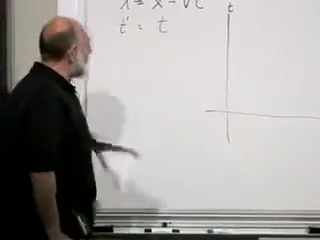
\includegraphics[width=0.72\textwidth]{lecture_04_figure_02.png}
\caption{伽利略變換與初始的$t$-$x$網格。運動的原點會沿著$x=vt$前進，而兩個參考系仍共用相同的等時線。}
\lectureframe{00:03:06}
\end{figure}

由式~\eqref{eq:l4-galilean}解出不帶撇號的座標，得到
\begin{align}
x&=x'+vt'=x'+vt, & t&=t'.
\end{align}
逆變換的形式相同，只要將$v$換成$-v$即可。如果列車相對車站向前運動，那麼車站相對列車便向後運動。在狹義相對論中，這種互易性依然成立，但普適時間則不成立。

\section{洛倫茲修正}

伽利略變換無法使光速在每個慣性參考系中都相同。修正後的關係式先寫成$c=1$單位制下的形式：
\begin{align}
x'&=\frac{x-vt}{\sqrt{1-v^2}}, &
t'&=\frac{t-vx}{\sqrt{1-v^2}}.
\label{eq:l4-lorentz-natural}
\end{align}
恢復一般單位制後，得到
\begin{align}
x'&=\frac{x-vt}{\sqrt{1-v^2/c^2}}, &
t'&=\frac{t-vx/c^2}{\sqrt{1-v^2/c^2}}.
\label{eq:l4-lorentz-c}
\end{align}

\begin{figure}[H]
\centering
\includegraphics[width=0.74\textwidth]{lecture_04_figure_05.png}
\caption{補回$c$因子的洛倫茲變換。}
\lectureframe{00:09:10}
\end{figure}

當$v\ll c$時，在適用牛頓力學的情況下，$v^2/c^2$和$vx/c^2$都很小。此時，式~\eqref{eq:l4-lorentz-c}便還原為伽利略變換的結果。相對論並未摒棄牛頓運動學，而是指出了它的適用範圍。

當$v=c$時，分母為零。慣性參考系不可能相對另一個慣性參考系以光速運動。遠低於此極限時，修正很小；但接近極限時，$x$與$t$的混合便無可避免。

運動方向選在$x$，因此橫向座標不變：
\begin{equation}
y'=y,\qquad z'=z.
\end{equation}
可以用以下方式理解原因：在列車和月台上各放一根相同的橫向米尺。一位以兩個參考系速度中間值運動的觀測者，會看到兩根尺以大小相等、方向相反的速度彼此接近。這個安排沒有任何特徵會使其中一根橫向米尺比另一根短。

\section{沿光錐方向的洛倫茲變換}

式~\eqref{eq:l4-lorentz-natural}還有一種幾何上的讀法。將其中兩個方程相加：
\begin{align}
t'+x'
&=\frac{(t-vx)+(x-vt)}{\sqrt{1-v^2}}\\
&=(t+x)\frac{1-v}{\sqrt{1-v^2}}\\
&=(t+x)\sqrt{\frac{1-v}{1+v}}.
\label{eq:l4-null-plus}
\end{align}
再以相反的順序相減：
\begin{align}
t'-x'
&=\frac{(t-vx)-(x-vt)}{\sqrt{1-v^2}}\\
&=(t-x)\frac{1+v}{\sqrt{1-v^2}}\\
&=(t-x)\sqrt{\frac{1+v}{1-v}}.
\label{eq:l4-null-minus}
\end{align}

\begin{figure}[H]
\centering
\includegraphics[width=0.75\textwidth]{lecture_04_figure_06.png}
\caption{以零座標組合$t+x$和$t-x$重寫的洛倫茲變換。兩者的比例因子互為倒數。}
\lectureframe{00:18:45}
\end{figure}

組合$t+x$和$t-x$是沿著兩個$45^\circ$類光方向的座標。洛倫茲推進會壓縮其中一個方向，並以互為倒數的因子拉伸另一個方向。兩個方向都不會偏離$45^\circ$。因此光線仍是光線；這正是光速不變性在時空中的圖像。

\begin{classroomqa}
\audiencequestion{位於中間的觀測者看到一個對稱的實驗，但這如何證明列車與月台上的觀測者也會得到相同結果？\lecturetimestamp{00:20:48}}
\lecturerresponse{這裡還用到另一項事實：事件是否重合是不變的。如果兩根尺的端點相遇，那次相遇就是一個時空事件。每位慣性觀測者都可以為它指定不同的座標，但沒有人能把一次重合拆成發生在兩個不同位置的事件。在相應端點相遇處發出的閃光，能讓這些事件在實際上被探測到。中間參考系的對稱性，加上兩個端點相遇事件的不變性，便確立了兩根尺的橫向長度相同。}
\end{classroomqa}

\begin{classroomqa}
\audiencequestion{代表中間參考系的騎腳踏車者，必須實際位於兩根尺的中點嗎？\lecturetimestamp{00:22:25}}
\lecturerresponse{不必。參考系是一整個由觀測者和時鐘構成的網絡，不是某個位置上的一隻眼睛。騎腳踏車者可以稍後才收到端點發出的閃光，再推斷閃光的發射位置。關鍵是每個發射事件在時空中的位置，而不是光最後在哪裡被接收。}
\end{classroomqa}

連續速度的合成也是同一變換的推論之一，但這部分刻意留到下一講再談。現在要做的是找出運動時鐘所測量的不變量。

\section{不變間隔}

普通笛卡兒座標軸旋轉時，量$x^2+y^2$保持不變。洛倫茲變換保留的則是另一種二次型。由式~\eqref{eq:l4-lorentz-natural}可得：
\begin{align}
t'^2-x'^2
&=\frac{(t-vx)^2-(x-vt)^2}{1-v^2}\\
&=\frac{t^2-2vtx+v^2x^2-x^2+2vtx-v^2t^2}{1-v^2}\\
&=t^2-x^2.
\label{eq:l4-interval}
\end{align}
混合項彼此抵消，剩下的分子則含有公因子$1-v^2$。

\begin{figure}[H]
\centering
\includegraphics[width=0.76\textwidth]{lecture_04_figure_07.png}
\caption{黑板上推導$t'^2-x'^2=t^2-x^2$的過程。}
\lectureframe{00:33:15}
\end{figure}

在三維空間中，不變量為
\begin{equation}
t'^2-x'^2-y'^2-z'^2=t^2-x^2-y^2-z^2
\end{equation}
此處採用$c=1$單位制。更一般地，對兩個事件，我們使用座標差：
\begin{equation}
\Delta s^2
=c^2\Delta t^2-\Delta x^2-\Delta y^2-\Delta z^2.
\label{eq:l4-spacetime-interval}
\end{equation}
每位慣性觀測者對這個數值都一致，儘管他們對時間項和空間項各自的數值並不一致。

\section{固有時與運動時鐘}

想像一個由靜止觀測者組成的格點，他們已透過交換光訊號將時鐘同步。他們的時鐘讀數定義了座標時間$t$。現在讓一只手錶穿過這個格點。手錶沿著自己的世界線前進，其自身的讀數就是固有時。

對兩個類時分離的事件，定義
\begin{equation}
c^2\Delta\tau^2
=c^2\Delta t^2-\Delta x^2-\Delta y^2-\Delta z^2.
\label{eq:l4-proper-time}
\end{equation}
在一維空間且採用$c=1$單位制時，這個定義簡化為
\begin{equation}
\Delta\tau=\sqrt{\Delta t^2-\Delta x^2}.
\end{equation}
它的平方根形式類似普通距離的公式，但負號改變了幾何性質。

有三種情況：
\begin{align}
\Delta t^2-\Delta x^2 &>0 &&\text{timelike},\\
\Delta t^2-\Delta x^2 &=0 &&\text{lightlike},\\
\Delta t^2-\Delta x^2 &<0 &&\text{spacelike}.
\end{align}
在光錐內部，固有時為實數。在光錐上，也就是$x=\pm t$的位置，即使兩個事件不必重合，固有時仍為零。光線恰好可以連接這樣的事件。在光錐外部，間隔是類空的；用實數固有距離$\sqrt{\Delta x^2-\Delta t^2}$描述會比用虛數的時鐘時間恰當。

\begin{figure}[H]
\centering
\includegraphics[width=0.73\textwidth]{lecture_04_figure_08.png}

\vspace{0.8em}

\begin{tikzpicture}[x=1.0cm,y=1.0cm]
\draw[->] (-3.3,0) -- (3.3,0) node[right] {$x$};
\draw[->] (0,-0.4) -- (0,4.0) node[above] {$t$};
\draw[thick] (0,0) -- (3.0,3.0) node[above right] {$x=t$};
\draw[thick] (0,0) -- (-3.0,3.0) node[above left] {$x=-t$};
\node at (0,2.0) {timelike};
\node at (2.25,1.05) {spacelike};
\node at (-2.25,1.05) {spacelike};
\end{tikzpicture}
\caption{黑板上的光錐，以及對類時、類光與類空間隔的清楚分類。}
\lectureframe{00:38:40}
\end{figure}

為什麼式~\eqref{eq:l4-proper-time}等於時鐘讀數？對靜止的時鐘而言，$\Delta x=0$，所以$\Delta\tau=\Delta t$。對等速運動的時鐘，選擇一個該時鐘靜止的帶撇號參考系。在那個參考系中，$\Delta x'=0$，而不變性給出
\begin{equation}
\Delta\tau
=\sqrt{\Delta t'^2-\Delta x'^2}
=\Delta t'.
\end{equation}
因此，運動時鐘所記錄的就是固有時。

\begin{classroomqa}
\audiencequestion{``事件之間的間隔''和``時鐘的讀數''是同一事物的兩種說法嗎？
\lecturetimestamp{00:44:49}}
\lecturerresponse{理想時鐘若沿慣性運動從一個事件行至另一個事件，兩者便相等。不變間隔是幾何量；共動時鐘兩端讀數的差則是對它的物理測量。靜止的座標時鐘通常會記錄不同的座標時間間隔。}
\end{classroomqa}

\section{時間膨脹與同時性}

考慮運動參考系的原點。它的世界線滿足
\begin{equation}
x'=0,\qquad x=vt.
\end{equation}
同一條傾斜直線既是運動時鐘的路徑，也是$t'$軸。

\begin{figure}[H]
\centering
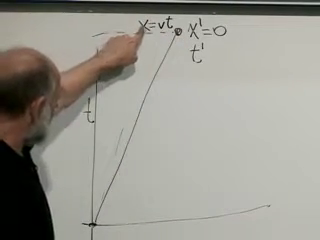
\includegraphics[width=0.72\textwidth]{lecture_04_figure_03.png}
\caption{運動原點：$x=vt$、$x'=0$和$t'$軸，都是描述同一條世界線的方式。}
\lectureframe{00:48:18}
\end{figure}

將不變間隔用於共同原點與該世界線上稍後的一點：
\begin{align}
t'^2-x'^2&=t^2-x^2,\\
t'^2&=t^2-v^2t^2,\\
t'&=t\sqrt{1-v^2}.
\label{eq:l4-time-dilation-natural}
\end{align}
補回$c$後，得到
\begin{equation}
\Delta\tau=\Delta t\sqrt{1-\frac{v^2}{c^2}}
=\frac{\Delta t}{\gamma},
\qquad
\gamma=\frac{1}{\sqrt{1-v^2/c^2}}.
\label{eq:l4-time-dilation}
\end{equation}

\begin{figure}[H]
\centering
\includegraphics[width=0.73\textwidth]{lecture_04_figure_09.png}
\caption{黑板上的時間膨脹結果：採用$c=1$單位制時，運動時鐘累積的固有時為$t'=t\sqrt{1-v^2}$。}
\lectureframe{00:50:45}
\end{figure}

靜止觀測者認為運動時鐘走得較慢。互易性要求運動觀測者也認為靜止時鐘走得較慢。這並不矛盾，因為兩種描述比較的是不同的遠距事件。

事實上，式~\eqref{eq:l4-lorentz-natural}中，$t'$為常數時滿足
\begin{equation}
t-vx=\text{constant}.
\label{eq:l4-simultaneity}
\end{equation}
運動觀測者的同時線相對於水平線$t=\text{constant}$是傾斜的。每位觀測者都把遠方時鐘讀數的不同組合視為同時。只要看清這項差異，時鐘彼此變慢的說法便不矛盾。

\begin{figure}[H]
\centering
\begin{tikzpicture}[x=1cm,y=1cm]
\draw[->] (0,0) -- (0,4.2) node[above] {$t$};
\draw[->] (0,0) -- (5.2,0) node[right] {$x$};
\draw[thick,->] (0,0) -- (2.4,3.8) node[above] {$x'=0$};
\draw[dashed] (0,2.8) -- (4.8,2.8)
  node[right] {$t=\mathrm{const}$};
\draw[thick] (0.15,1.05) -- (4.7,2.35)
  node[right] {$t'=\mathrm{const}$};
\draw[thick] (3.4,0) -- (3.4,3.8);
\fill (3.4,2.8) circle (0.045);
\fill (3.4,1.98) circle (0.045);
\end{tikzpicture}
\caption{互易的時間膨脹，是在不同的同時性切片上比較時鐘讀數。}
\end{figure}

\section{雙胞胎的路徑}

兩位雙胞胎從同一事件出發。一位留在$x=0$。另一位以速度$v$向外行進，接著掉頭，再以相同速度返回。重逢時，他們比較所有可作為時鐘的物理過程：手錶、心跳、新陳代謝，或衰老本身。

令旅程的每一段在留守者的參考系中都歷時$T$座標時間。留守雙胞胎的固有時為
\begin{equation}
\tau_{\mathrm{home}}=2T.
\end{equation}
掉頭事件的座標為$(vT,T)$。因此，外出路程所累積的固有時為
\begin{align}
\tau_{\mathrm{leg}}
&=\sqrt{T^2-v^2T^2}
=T\sqrt{1-v^2}.
\end{align}
回程也累積相同的固有時，所以
\begin{equation}
\tau_{\mathrm{travel}}=2T\sqrt{1-v^2}<2T.
\label{eq:l4-twin}
\end{equation}

\begin{figure}[H]
\centering
\includegraphics[width=0.73\textwidth]{lecture_04_figure_10.png}

\vspace{0.8em}

\begin{tikzpicture}[x=1.1cm,y=1cm]
\draw[->] (-0.2,0) -- (3.4,0) node[right] {$x$};
\draw[->] (0,-0.1) -- (0,4.4) node[above] {$t$};
\draw[very thick] (0,0) -- (0,4);
\draw[very thick] (0,0) -- (2.2,2) -- (0,4);
\draw[dashed] (0,2) -- (2.2,2);
\node[left] at (0,2) {$T$};
\node[left] at (0,4) {$2T$};
\node[below right] at (1.1,1.0) {$v$};
\node[above right] at (1.1,3.0) {$-v$};
\end{tikzpicture}
\caption{留守者的世界線與雙胞胎外出的兩段路程。它們的固有時不同，因為它們是穿越時空的不同路徑。}
\lectureframe{00:59:35}
\end{figure}

雙胞胎年齡不同並不矛盾。旅行路徑包含一次轉向，因此無法透過單一慣性參考系對稱性，將它與留守者的直線路徑聯繫起來。在普通歐幾里得幾何中，連接兩點的直線路徑與折線路徑長度也不同。閔可夫斯基幾何中，哪條路徑的間隔較大恰好相反，但比較仍是幾何上的比較。

\section{加速度與理想時鐘}

\begin{classroomqa}
\audiencequestion{在掉頭時，物理情況有所不同，旅行者也會加速。這會使時鐘計算失效嗎？
\lecturetimestamp{01:02:19}}
\lecturerresponse{加速度是真實的，也有助於辨認不對稱性；不應把它搪塞過去。尖銳的轉角只是理想化的圖示，可以改成有限時間內平順完成的轉向。還需要一項物理假設：尺寸足夠小、構造良好的時鐘不受適度加速度影響，並會繼續記錄固有時。大型或脆弱的時鐘可能變形或損壞，但那是時鐘機制的缺陷，而非時空間隔的問題。}
\end{classroomqa}

理想時鐘這項假設無法單從洛倫茲變換推導出來，而是透過實際時鐘機制的行為加以檢驗。原子比一個橫跨數百英里的時鐘更接近理想時鐘，因為緊密的機制較不容易在加速度或重力作用下變形。只提到廣義相對論，並不能消除這個物理問題；我們仍須了解所選機制如何對環境作出反應。

\begin{classroomqa}
\audiencequestion{能否把加速軌跡分成許多短區段，使每一段仍可使用慣性分析？\lecturetimestamp{01:09:08}}
\lecturerresponse{可以。將曲線分成短而近似筆直的區段，計算每一段的固有時，再把結果相加。這相當於在時空中用許多短線段求出普通曲線的長度。取連續極限時，
\[
\tau=\int \sqrt{1-\frac{v(t)^2}{c^2}}\,dt,
\]
適用於以慣性座標系描述的平直時空中的運動。}
\end{classroomqa}

\section{雙胞胎看到的情形}

可以透過發送光脈衝，實際比較最後的時鐘讀數。在兩條世界線上每隔一秒固有時做一個記號，並讓每位雙胞胎在每個記號處發出脈衝。外出途中，收到對方脈衝的間隔會拉長；回程時，脈衝則會密集到達。這就是直接呈現在時空圖上的相對論多普勒效應。

\begin{figure}[H]
\centering
\includegraphics[width=0.73\textwidth]{lecture_04_figure_11.png}
\caption{留守者與旅行者的世界線之間交換的光訊號。外出途中稀疏到達的脈衝，以及回程途中密集到達的脈衝，涵蓋了每一個發出的脈衝。}
\lectureframe{01:12:55}
\end{figure}

故事中的任何參考系都沒有消失。每位觀測者最終都會收到對方發出的所有脈衝，但接收速率取決於相對運動。對兩條路徑而言，外出時的紅移與回程時的藍移持續時間不同，因此把收到的脈衝全部計數後，仍會符合固有時的比較結果。

\begin{classroomqa}
\audiencequestion{回程的旅行者若收到藍移的光，會不會收集到比光源發出時更多的能量？\lecturetimestamp{01:13:50}}
\lecturerresponse{要回答這個問題，必須先建立能量的相對論定義及其參考系依賴性；目前尚未討論這些內容。這個問題問得合理，但單靠座標和脈衝計數不足以釐清能量帳目，尤其對加速中的觀測者更是如此。因此應該暫緩回答，而不是猜測。}
\end{classroomqa}

\section{閉合的空間方向}

\begin{classroomqa}
\audiencequestion{假設有一個緊緻化的空間方向。雙胞胎能否沿這個方向等速運動、回到出發地，完全不經歷加速度？那麼，兩位雙胞胎有何不同？\lecturetimestamp{01:15:14}}
\lecturerresponse{應將空間本身想像成一個圓柱面，而不是彎曲後嵌入更大空間中的一張面；這裡不需要徑向加速度。然而，返回的觀測者仍會遇到同一地點反覆出現這項全域特性。這顯示存在某種不對稱性，但若要完整回答，就必須仔細處理具有空間識別的狹義相對論。這裡先把問題保留為開放問題，不臨時拼湊答案。}
\end{classroomqa}

\begin{figure}[H]
\centering
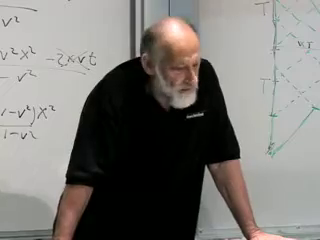
\includegraphics[width=0.72\textwidth]{lecture_04_figure_04.png}

\vspace{0.8em}

\begin{tikzpicture}[x=1cm,y=1cm]
\draw[thick] (0,0) ellipse (1.3 and 0.35);
\draw[thick] (-1.3,0) -- (-1.3,-3.1);
\draw[thick] (1.3,0) -- (1.3,-3.1);
\draw[thick] (0,-3.1) ellipse (1.3 and 0.35);
\draw[->,very thick] (0.0,0.38) arc (90:-210:1.38 and 0.42);
\node[right] at (1.65,-1.5) {compact spatial direction};
\end{tikzpicture}
\caption{黑板上畫出的緊緻空間問題，並以清楚的內在圓柱面呈現。這是關於全域識別的問題，而非關於在額外的徑向維度中繞著圓柱面運動。}
\lectureframe{01:17:56}
\end{figure}

\section{長度是在同時性切片上測量的}

處理狹義相對論問題時，先畫出時空圖。取一根在不帶撇號參考系中靜止的米尺，兩端位於$x=0$和$x=1$。隨著時間經過，兩個端點各自描出垂直的世界線。米尺在兩條世界線之間掃出一條帶狀區域。

運動觀測者必須在運動時間$t'$的同一時刻測量兩個端點。由式~\eqref{eq:l4-simultaneity}可知，通過原點且滿足$t'=0$的切片，在$c=1$單位制下符合
\begin{equation}
t=vx
\end{equation}
這個切片與右端點$x=1$的世界線相交於$t=v$。

\begin{figure}[H]
\centering
\includegraphics[width=0.73\textwidth]{lecture_04_figure_12.png}

\vspace{0.8em}

\begin{tikzpicture}[x=1.55cm,y=1.15cm]
\draw[->] (-0.5,0) -- (3.1,0) node[right] {$x$};
\draw[->] (0,0) -- (0,3.8) node[above] {$t$};
\draw[very thick,red] (0,0) -- (0,3.3);
\draw[very thick,red] (2.15,0) -- (2.15,3.3);
\fill[red!12] (0,0) rectangle (2.15,3.3);
\draw[very thick,green!50!black] (0,0) -- (1.2,3.1)
  node[above] {$x=vt$};
\draw[very thick,blue] (0,0) -- (2.15,1.15)
  node[right] {$t'=0$};
\fill (2.15,1.15) circle (0.045);
\node[right] at (2.22,1.35) {$(x,t)=(1,v)$};
\node[below] at (2.15,0) {$1$};
\end{tikzpicture}
\caption{靜止的尺在時空中掃出一條帶狀區域。運動觀測者測得的長度，是尺的兩端在同一個$t'=\mathrm{const}$切片上的間距。}
\lectureframe{01:24:20}
\end{figure}

選取的端點間隔是類空的，因此使用不變量的正空間形式：
\begin{equation}
x'^2-t'^2=x^2-t^2.
\end{equation}
在選取的端點處，$t'=0$、$x=1$，且$t=v$。因此
\begin{align}
x'^2&=1-v^2,\\
x'&=\sqrt{1-v^2}.
\end{align}
於是，靜止長度為$L$的尺，在運動參考系中測得的長度為
\begin{equation}
L'=L\sqrt{1-v^2/c^2}=\frac{L}{\gamma}.
\label{eq:l4-length-contraction}
\end{equation}

\begin{figure}[H]
\centering
\includegraphics[width=0.76\textwidth]{lecture_04_figure_13.png}
\caption{完成的長度收縮作圖，以及靜止長度為一單位時黑板上得到的結果$x'=\sqrt{1-v^2}$。}
\lectureframe{01:28:10}
\end{figure}

互易的說法也成立：月台上的觀測者測得列車上的縱向米尺較短。再一次，兩位觀測者選取了不同的同時端點事件，因此互易性並不矛盾。

\section{最後的問題}

\begin{classroomqa}
\audiencequestion{除了光，還有什麼會以光速傳播？特別是引力呢？\lecturetimestamp{01:29:29}}
\lecturerresponse{廣義相對論預言，引力波會以$c$傳播。在這場講座舉行時，相關證據來自雙脈衝星等系統的間接觀測；當時尚未直接探測到引力波。\editorialnote{這場2006講座之後，實驗情況有所改變。LIGO 在 2015 年直接探測到 GW150914；而在 2017 年對 GW170817 及其電磁對應訊號的聯合觀測，顯示引力與光的傳播速度差異僅在 $10^{15}$ 分之幾的量級。參見 \url{https://ligo.org/detections/gw150914/} 和
\url{https://doi.org/10.1103/PhysRevLett.119.251302}。}}
\end{classroomqa}

\begin{classroomqa}
\audiencequestion{太空人能否在少於以光年表示的距離數值所對應的固有時內，穿越數光年的距離？這是否代表他移動得比光還快？\lecturetimestamp{01:30:38}}
\lecturerresponse{太空人的固有時為
$\sqrt{\Delta t^2-\Delta x^2}$，小於座標時間$\Delta t$。在太空人的慣性參考系中，恆星之間的距離會發生洛倫茲收縮。恆星以速度$-v$運動，並未超過光速；只是需要穿越的收縮後距離較短。}
\end{classroomqa}

如果太空人從靜止開始加速，描述就會隨著一系列瞬時慣性參考系而改變。在這段轉換過程中，恆星之間的距離可能改變。不能用單一固定的洛倫茲變換描述整段加速歷程，但總固有時仍可由沿世界線累加各段貢獻求得。真實的雙胞胎也是如此：他會起航、轉向並減速，而不是一出生就以巡航速度行進。

\begin{classroomqa}
\audiencequestion{這些難題是否源於把時間視為特殊的存在？我們是否必須稱它為第四維？\lecturetimestamp{01:36:43}}
\lecturerresponse{不必一開始就採用「時間是第四維」這句口號。洛倫茲變換本身就迫使空間與時間混合，而間隔$t^2-x^2-y^2-z^2$則把兩者視為同一幾何的組成部分，只是時間項與空間項的符號不同。在低速下，這種混合可以忽略，熟悉的牛頓直覺便會恢復。但在相對論速度下，空間與時間不能被視為根本上彼此獨立。}
\end{classroomqa}

因此，時間膨脹、長度收縮、雙胞胎的比較，以及縮短的旅行時間，並非彼此無關的技巧。它們都源自三個做法：辨明要比較的事件、畫出事件的時空幾何，並使用不變間隔。
\chapter{火球、參考系與四維向量}

我們先從高能碰撞討論中留下的一個問題談起。兩個重原子核碰撞後形成的，是一個劇烈變化的物體，而非寧靜的天文黑洞。那麼，用視界描述這種碰撞究竟有何意義？答案會帶我們先認識強耦合物質的五維圖像，再探討一系列加速器的實際問題，最後回到狹義相對論的幾何。到最後，速度和動量都成了四維向量，而能量也與動量的三個分量並列。

\section{第五維中的火球}

\begin{classroomqa}
\audiencequestion{碰撞產生的物體並不穩定，形狀也會改變。這樣複雜的物體怎麼能稱為黑洞？}
\lecturerresponse{想像第五個空間方向延伸於地板和天花板之間。該方向上的引力會把激發態拉向地板。碰撞在那裡沉積了一團高熱能量；它會擴散、改變形狀，卻仍可具有視界、溫度和熵。}
\end{classroomqa}

想像粒子，或者更形象地說，小弦，在這個五維世界中運動。落向地板的激發態，在四維中呈現為強子：質子、中子、介子，以及其他延展的複合物體。附著在天花板附近的激發態則呈現得較為基本。因此，垂直位置是一種以幾何方式編碼尺度的手段：地板代表長距離的強子區域，天花板則代表短距離的自由度。

兩個強子碰撞時，地板附近的兩個物體相撞，激起大量能量。產物不是剛體，而是一團帶有視界的高熱物質，彷彿五維引力場中的一灘水。它既不是普通四維空間中的天文黑洞，也不是附著在天花板上的普朗克尺度黑洞，而是地板附近強作用火球的引力描述。

在高能下，入射原子核會因洛倫茲收縮而變成薄薄的煎餅狀。它們碰撞後，將能量沉積在一小塊區域，並產生逐漸趨近平衡的流體。夸克--膠子電漿的小黏滯性，是它令人驚訝的特徵之一。在五維描述中，同樣的演化就是扭曲視界的弛豫。

\begin{figure}[H]
\centering
\includegraphics[width=0.82\textwidth]{lecture_05_figure_01.png}
\caption{第五維的地板與天花板圖像。碰撞後，中央這團帶有視界的物質沿著地板擴散。}
\lectureframe{00:04:22}
\end{figure}

視界不會永遠存在。霍金輻射會帶走能量；在四維描述中，這些輻射就是碰撞後湧現的一簇簇普通強子。用這種語言來說，探測器事件中的數千條徑跡，就是從對偶黑洞中蒸發出來的粒子。

\subsection{額外維度是真實存在的嗎？}

\begin{classroomqa}
\audiencequestion{第五維是空間維度嗎？圖中地板與天花板之間的那條線，真的是沿著這個方向延伸嗎？}
\lecturerresponse{是的。這是類空方向，而在該五維幾何中畫出的曲面就是視界。至於額外方向是否``真實存在''，或者只是等價的數學描述，則是更深一層的問題。}
\end{classroomqa}

有用的說法不是引力取代了量子色動力學，而是兩種語言可能描述同一套物理。在四維語言中，這是一團由夸克和膠子組成的高熱火球，沒有通常意義下的引力場。在五維語言中，則有引力和視界。如果這種對應成立，那麼只要兩種計算都做得到，嚴謹的 QCD 計算就必須和對偶的引力計算一致。

\begin{classroomqa}
\audiencequestion{QCD 中既沒有引力，也沒有視界。黑洞圖像是在加入新物理，還是只用另一種方式描述火球？}
\lecturerresponse{在四維中，它是夸克和膠子組成的電漿；在五維版本中，則有帶視界的引力描述。這種描述的優勢在於計算。強耦合 QCD 極難計算，但某些視界性質---尤其是黏滯性---相對容易計算。}
\end{classroomqa}

``真實維度''和``數學類比''之間的區別，不必先有定論，這種描述才有用。當某個結構能把其他變數整合成一組更簡潔、更連貫的定律時，它便具有物理解釋的價值。儘管如此，也不應誇大其意義：規範／引力對偶性應用於觀測到的夸克--膠子電漿時，提供的是強耦合動力學的模型，並不能證明現實世界的 QCD 已知具有精確的引力對偶。\editorialnote{這項限定明確說明了 QCD 應用在現代物理中的定位；它不會改變此處闡述的五維機制。}

\section{為什麼對撞機要讓束流互撞}

現在來看幾個實際問題：為什麼要讓兩束運動中的粒子束互撞，而不是讓一束粒子撞上靜止靶？為什麼環形加速器這麼大？為什麼電子和質子的處理方式不同？這些問題都與相對論能量有關。

\begin{classroomqa}
\audiencequestion{為什麼要讓兩束粒子束互撞，而不是用一束高能粒子束撞擊靜止靶？}
\lecturerresponse{產生新粒子所需的能量，取決於質心系中可用的能量。兩束能量相等、方向相反的相對論性粒子束，總動量為零，因此幾乎所有能量都可用於碰撞。若靶固定，入射能量中有很大一部分只能成為質心的運動。}
\end{classroomqa}

對於兩個動量大小為\(p\)、方向相反的超相對論性粒子，在\(c=1\)單位下，講義中的估算為
\begin{equation}
E_{\mathrm{cm}}^{\mathrm{collider}}\simeq 2p.
\end{equation}
固定靶的相應估算則只隨束流動量的平方根增加，
\begin{equation}
E_{\mathrm{cm}}^{\mathrm{fixed}}\sim \sqrt{mp}.
\end{equation}
關鍵在於標度關係，而非省略的數值因子：束流能量加倍，對撞機的質心能量也加倍；固定靶的質心能量則只增加為原來的平方根倍。

用不變量計算，可以精確比較兩者。若\(P_1\)和\(P_2\)是入射四維動量，則
\begin{equation}
s=(P_1+P_2)^2,
\qquad E_{\mathrm{cm}}=\sqrt{s}.
\end{equation}
對於能量為\(E\)、等能量且反向傳播的兩束粒子，空間動量彼此抵消，因此\(\sqrt{s}=2E\)。若能量為\(E\gg m\)的入射粒子撞上靜止的等質量靶，則
\begin{equation}
s=2m^2+2mE,
\qquad
\sqrt{s}\simeq \sqrt{2mE}
\qquad (c=1).
\end{equation}
這個簡短的不變量推導補上了口頭估算中省略的因子。\editorialnote{列出這項推導，是為了讓講義中的標度論證可以重現。}

\begin{classroomqa}
\audiencequestion{環形加速器非得這麼大不可，有什麼根本原因嗎？能不能讓同一束粒子多繞幾圈，通過較小的機器？}
\lecturerresponse{磁場和材料都會形成限制。粒子每公尺所能增加的能量有限，因此能量更高的機器需要更長的有效加速距離。環越小，所需的橫向加速度也越大；而帶電粒子在加速時會輻射。環太小時，束流輻射掉能量的速度就會和機器供應能量的速度一樣快。}
\end{classroomqa}

偏轉關係近似為
\begin{equation}
p=qBR,
\end{equation}
因此，在磁場\(B\)固定時，動量\(p\)越大，所需半徑\(R\)也越大。提高束流能量的工作由射頻腔完成；磁鐵則負責使束流偏轉並聚焦。大致來說，黑板上的結論仍然成立：場強和輻射損失使我們無法把任意高能的加速器塞進小環裡。

即使速率不變，圓周運動仍有加速度，因為速度方向持續改變。加速中的電荷會發射同步輻射。直線加速器沒有持續轉向所造成的損失，但短暫的加速推進本身也並非完全沒有輻射。環形加速器接受轉向帶來的代價，換取每一圈都能重複使用同一套設備。

\begin{classroomqa}
\audiencequestion{為什麼電子會和 SLAC 的直線加速器相聯，而環形高能對撞機卻使用質子或其他強子？}
\lecturerresponse{電子的質量小得多。在相同的高能量下，電子的洛倫茲因子大得多；環形加速會使它們發出強得多的輻射。較重的質子可以在環中反覆運行，每經過一次就增加一些能量，直到同步輻射損失變得難以承受。}
\end{classroomqa}

在能量和環半徑固定時，輻射功率對粒子質量的依賴非常陡峭，
\begin{equation}
P_{\mathrm{sync}}\propto \frac{E^4}{m^4R^2}.
\end{equation}
因此，電子--質子的差異，遠比``較輕的粒子跑得比較快''這句話所暗示的更大得多：兩束粒子的速度都可能已非常接近\(c\)，但它們的洛倫茲因子和輻射損失卻大不相同。\editorialnote{偏轉關係和同步輻射的標度律，讓講義中的加速器定性論證有了精確的表述；這些推導並未在黑板上完成。}

\begin{classroomqa}
\audiencequestion{為什麼不也用直線加速器加速強子？}
\lecturerresponse{可以。難處在於所需長度。在環形加速器中，同一粒子會多次通過加速結構；要達到相同效果，直線強子加速器就得長得驚人。實用的折衷方案是採用大型環形加速器，讓環大到質子輻射仍在可容忍範圍內。}
\end{classroomqa}

這些加速器問題正好說明，為什麼牛頓力學的規則不敷使用。現在我們回到狹義相對論，建立一套能有系統地比較這些情況的語言。

\section{車庫與加長型禮車}

想像一座約十二英尺長的車庫，以及一輛約二十英尺長的加長型禮車。司機不斷加速，直到禮車因洛倫茲收縮而變短，希望它能塞進車庫。在車庫參考系中，運動中的禮車較短，因此看起來塞得進去。然而在禮車參考系中，運動中的車庫較短，因此看起來塞不進去。整輛禮車到底能不能完全在車庫裡？

把兩扇門都打開，免得撞上牆壁的問題分散我們的注意力。說禮車在車庫裡，意思是它的車頭和車尾\emph{同時}都在車庫內。整個謎題的關鍵就在「同時」這個詞。

畫一張時空圖，讓\(t\)軸垂直、\(x\)軸水平。在\(c=1\)單位下，光線形成\(45^\circ\)光錐。車庫靜止，因此兩扇門的世界線是垂直線。禮車的車頭和車尾則沿著兩條平行斜線運動。運動參考系的\(t'\)軸朝光錐方向傾斜，而其同時線平行於傾斜的\(x'\)軸。

\begin{figure}[H]
\centering
\includegraphics[width=0.82\textwidth]{lecture_05_figure_02.png}
\caption{完整的車庫--禮車時空圖。垂直線標示車庫的邊界；斜線描繪禮車的兩端。水平和傾斜的截線，分別代表兩個參考系不同的同時性切面。}
\lectureframe{00:31:05}
\end{figure}

在車庫參考系中，一條水平線可以在兩條車庫門的世界線之間，穿過禮車兩端的世界線。在車庫的那個時刻，車尾已進入車庫，車頭還沒出去。收縮後的禮車整輛都在車庫內。

在禮車參考系中，相關的同時事件位於一條斜線上。從車尾進入車庫的事件畫出這條線；線與車頭世界線相交時，車頭早已通過遠端的門。依照禮車自身的同時性，整輛禮車從未完全位於車庫內。兩種說法都成立，因為各自比較的是不同的一對事件。

\begin{classroomqa}
\audiencequestion{兩條綠色世界線和它們之間的水平線段構成平行四邊形嗎？那條黑色線段就是車輛的長度嗎？}
\lecturerresponse{水平線段代表洛倫茲收縮後的長度，因為它的兩個端點在車庫參考系中同時。固有長度則由禮車參考系中同時的兩個端點決定，這兩點位於平行於\(x'\)的直線上。兩種測量是在同一對世界線上取不同的截線。}
\end{classroomqa}

若固有長度為\(L_0\)，車庫參考系中的水平截線長度就是\begin{equation}
L=\frac{L_0}{\gamma},
\qquad
\gamma=\frac{1}{\sqrt{1-v^2/c^2}}.
\end{equation}
單靠公式無法解開這個悖論；圖可以，因為圖顯示了比較的是哪些事件。每當相對論的問題似乎導出兩個互不相容的答案，就要留意其中是否暗中用到了「``同時''」這個概念。

\section{四個座標與兩種指標位置}

要從謎題轉向運動定律，我們需要一套能反映幾何的記號。把座標寫成
\begin{equation}
(X^1,X^2,X^3,X^0)=(x,y,z,t),
\qquad X^\mu=(x,y,z,t),
\end{equation}
其中，\(\mu\)依序取\(1,2,3,0\)。這個排列把時間放在書寫順序的最後，儘管它的指標是\(0\)，與黑板上採用的慣例相同。

\begin{classroomqa}
\audiencequestion{我們是令\(c=1\)嗎？如果恢復一般單位，時間座標是不是應該寫成\(ct\)？}
\lecturerresponse{是的。在建立幾何時，我們令\(c=1\)；遇到量綱或非相對論極限等問題時，再把\(c\)的因子放回去。使用慣常的長度單位時，時間座標是\(ct\)。}
\end{classroomqa}

同一個向量也可以用下指標表示。採用這裡的符號約定，
\begin{equation}
X_\mu=(-x,-y,-z,t).
\end{equation}
因此，降低指標會使三個空間分量的符號反轉，而時間分量的符號不變。例如，
\begin{equation}
X^\mu=(3,2,4,10)
\quad\Longrightarrow\quad
X_\mu=(-3,-2,-4,10).
\end{equation}
這不是兩個時空點，而是同一個幾何物體的兩種分量表示法。

\begin{classroomqa}
\audiencequestion{哪些分量是協變、哪些是逆變？標記應該寫成上標還是下標？}
\lecturerresponse{上指標分量是逆變的；下指標分量是協變的。課堂上有個好記的口訣：``co 在下，contra 在上。''物理學家也常直接說「上面」和「下面」。}
\end{classroomqa}

這套記號的優點，在不變縮併中一目了然：
\begin{equation}
X_\mu X^\mu=t^2-x^2-y^2-z^2.
\label{eq:l5-interval}
\end{equation}
用微分表示，就是
\begin{equation}
d\tau^2=dt^2-dx^2-dy^2-dz^2
\qquad (c=1).
\label{eq:l5-proper-time}
\end{equation}
對於類時運動，\(d\tau\)是沿著世界線運動的時鐘所記錄的時間。

同一個指標若在上方出現一次、下方出現一次，就表示要對該指標求和。愛因斯坦求和慣例將
\begin{equation}
\sum_{\mu}X_\mu X^\mu
\end{equation}
簡寫成式~\eqref{eq:l5-interval}中的形式。這不只是節省排版空間，也免去了在每個方程中手動重寫閔可夫斯基幾何交錯的正負號。

\begin{classroomqa}
\audiencequestion{\(\tau\)是固有時的標準符號嗎？}
\lecturerresponse{是的。有時也會用符號\(s\)，但\(\tau\)是表示固有時的標準選擇。}
\end{classroomqa}

\section{作為簡單對稱操作的旋轉}

洛倫茲推移會混合空間和時間。在研究那個矩陣之前，先來看較熟悉的操作：旋轉空間座標軸。如果相對運動方向不固定在某個軸上，我們可以先旋轉座標軸，讓該方向成為新的\(x\)軸，再施加已知的洛倫茲推移。因此，旋轉是構造的一部分，並非多餘的插曲。

繞\(z\)軸旋轉角度\(\theta\)時，
\begin{align}
x'&=x\cos\theta+y\sin\theta,\nonumber\\
y'&=-x\sin\theta+y\cos\theta,\label{eq:l5-rotation}\\
z'&=z.\nonumber
\end{align}
在\(\theta=0\)時，這些方程會給出\(x'=x\)和\(y'=y\)；在\(\theta=\pi/2\)時，則會以預期的符號互換兩個座標軸。

此變換會保持歐幾里得距離不變。令
\(c_\theta=\cos\theta\)和\(s_\theta=\sin\theta\)，則
\begin{align}
x'^2+y'^2
&=(xc_\theta+ys_\theta)^2+(-xs_\theta+yc_\theta)^2\nonumber\\
&=x^2(c_\theta^2+s_\theta^2)
  +y^2(s_\theta^2+c_\theta^2)\nonumber\\
&\quad+2xyc_\theta s_\theta-2xyc_\theta s_\theta\nonumber\\
&=x^2+y^2.
\end{align}
交叉項相消，因此\(c_\theta^2+s_\theta^2=1\)。又因為\(z'=z\)，整個長度\(x^2+y^2+z^2\)也保持不變。

同一組方程也可以寫成一個矩陣方程：
\begin{equation}
\begin{pmatrix}x'\\y'\\z'\end{pmatrix}
=
\underbrace{\begin{pmatrix}
\cos\theta&\sin\theta&0\\
-\sin\theta&\cos\theta&0\\
0&0&1
\end{pmatrix}}_{M}
\begin{pmatrix}x\\y\\z\end{pmatrix}.
\label{eq:l5-rotation-matrix}
\end{equation}
用指標記號表示則為
\begin{equation}
x'^i=M^i{}_{j}x^j,
\qquad i,j=1,2,3.
\end{equation}

\begin{figure}[H]
\centering
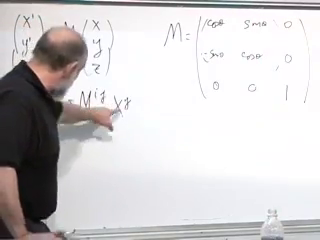
\includegraphics[width=0.82\textwidth]{lecture_05_figure_03.png}
\caption{空間旋轉的矩陣方程及其指標記號表示法。}
\lectureframe{01:00:40}
\end{figure}

\section{洛倫茲矩陣與速度合成}

沿\(x\)方向運動時，在\(c=1\)單位下，洛倫茲變換為
\begin{align}
x'&=\gamma_v(x-vt), & y'&=y,\nonumber\\
z'&=z, & t'&=\gamma_v(t-vx),
\end{align}
其中
\begin{equation}
\gamma_v=\frac{1}{\sqrt{1-v^2}}.
\end{equation}
若分量順序採用\((x,y,z,t)\)，則可寫成
\begin{equation}
\begin{pmatrix}x'\\y'\\z'\\t'\end{pmatrix}
=
\begin{pmatrix}
\gamma_v&0&0&-\gamma_vv\\
0&1&0&0\\
0&0&1&0\\
-\gamma_vv&0&0&\gamma_v
\end{pmatrix}
\begin{pmatrix}x\\y\\z\\t\end{pmatrix}.
\label{eq:l5-lorentz-matrix}
\end{equation}

\begin{figure}[H]
\centering
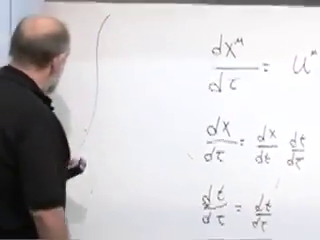
\includegraphics[width=0.82\textwidth]{lecture_05_figure_04.png}
\caption{\(4\times4\)洛倫茲矩陣。只有\(x\)和\(t\)分量會混合；\(y\)和\(z\)則保持不變。}
\lectureframe{01:04:40}
\end{figure}

矩陣乘法現在可以回答一個物理問題。假設有位觀察者以速度\(v\)相對於我們運動，另一位觀察者再以速度\(u\)相對於前一位觀察者運動，而且都沿同一軸。牛頓運動學會給出\(w=u+v\)，這樣一來，兩個\(3c/4\)的速度就可能合成為\(3c/2\)。相對論必須給出不同的規則。

洛倫茲推移中起作用的部分是\(2\times2\)矩陣：
\begin{equation}
B(v)=\gamma_v
\begin{pmatrix}1&-v\\-v&1\end{pmatrix}.
\end{equation}
將兩個推移複合，得到
\begin{align}
B(u)B(v)
&=\gamma_u\gamma_v
\begin{pmatrix}1&-u\\-u&1\end{pmatrix}
\begin{pmatrix}1&-v\\-v&1\end{pmatrix}\nonumber\\
&=\gamma_u\gamma_v
\begin{pmatrix}
1+uv&-(u+v)\\
-(u+v)&1+uv
\end{pmatrix}.
\label{eq:l5-composed-boost}
\end{align}
非對角元素與對角元素的比值，可用來求出合成推移的速度：
\begin{equation}
w=\frac{u+v}{1+uv}
\qquad(c=1).
\end{equation}
恢復量綱後，
\begin{equation}
w=\frac{u+v}{1+uv/c^2}.
\label{eq:l5-velocity-addition}
\end{equation}

\begin{figure}[H]
\centering
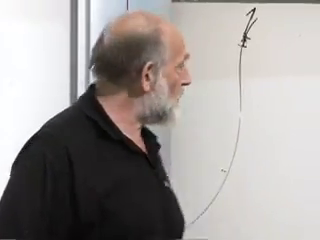
\includegraphics[width=0.82\textwidth]{lecture_05_figure_05.png}
\caption{複合推移的矩陣，以及自然單位下的速度\(w=(u+v)/(1+uv)\)。}
\lectureframe{01:15:35}
\end{figure}

若\(u\)和\(v\)都接近\(c\)，分子就趨近\(2c\)，分母則趨近\(2\)，所以\(w\)會趨近\(c\)，而非\(2c\)。更一般地說，式~\eqref{eq:l5-velocity-addition}會把亞光速輸入映成亞光速結果。矩陣乘法自動保證了速度上限。

\section{四維向量與普通速度為何不適用}

四維向量是指一種物體，其四個分量在旋轉和洛倫茲推移下的變換方式，與時空座標相同。若\(V^\mu\)是四維向量，依照我們的符號約定，
\begin{equation}
V_\mu=(-V^1,-V^2,-V^3,V^0),
\end{equation}
它的不變範數為
\begin{equation}
V_\mu V^\mu=(V^0)^2-(V^1)^2-(V^2)^2-(V^3)^2.
\end{equation}
對於兩個四維向量\(V^\mu\)和\(W^\mu\)，縮併
\begin{equation}
W_\mu V^\mu
=W^0V^0-W^1V^1-W^2V^2-W^3V^3
\end{equation}
也同樣是不變量。分量會隨參考系改變，縮併則不會。

普通速度只有三個分量：
\begin{equation}
\mathbf v=\left(\frac{dx}{dt},\frac{dy}{dt},\frac{dz}{dt}\right).
\end{equation}
光是附上\(dt/dt=1\)，並不能讓它成為有用的四維向量。如此一來，第四個分量只是平凡的數值，整個物體也不會依照洛倫茲變換作線性變換。座標時間\(t\)會因參考系而異，因此對\(t\)微分會破壞所需的變換律。

用固有時就能解決這個問題。沿著世界線定義
\begin{equation}
u^\mu=\frac{dX^\mu}{d\tau}.
\label{eq:l5-four-velocity}
\end{equation}
微分\(dX^\mu\)是四維向量，而\(d\tau\)是不變量，因此兩者之比也是四維向量。``固有''這個形容詞，指的是分母中的時鐘。

鏈鎖律將這個物體與普通速度連結起來：
\begin{equation}
\frac{dx}{d\tau}=\frac{dx}{dt}\frac{dt}{d\tau},
\end{equation}
對\(y\)和\(z\)也一樣。由式~\eqref{eq:l5-proper-time}可得
\begin{align}
\left(\frac{d\tau}{dt}\right)^2
&=1-\left(\frac{dx}{dt}\right)^2
    -\left(\frac{dy}{dt}\right)^2
    -\left(\frac{dz}{dt}\right)^2\nonumber\\
&=1-v^2
\qquad(c=1),
\end{align}
因此
\begin{equation}
\frac{dt}{d\tau}=\gamma_v=\frac{1}{\sqrt{1-v^2}}.
\end{equation}
四個分量為
\begin{equation}
u^i=\gamma_v v^i,
\qquad
u^0=\gamma_v
\qquad(c=1).
\label{eq:l5-four-velocity-components}
\end{equation}
在低速下，\(u^i\simeq v^i\)且\(u^0\simeq1\)。接近光速時，\(\gamma_v\)會無界增大，固有速度也就與普通速度大不相同。

\begin{figure}[H]
\centering
\includegraphics[width=0.82\textwidth]{lecture_05_figure_06.png}
\caption{以普通速度和洛倫茲因子表示的固有速度四個分量。}
\lectureframe{01:34:40}
\end{figure}

恢復慣用單位並使用\(X^0=ct\)，即可得到標準形式
\begin{equation}
U^\mu=(\gamma_v\mathbf v,\gamma_v c)
\end{equation}
這裡採用空間分量在前的排列順序。其不變範數為
\begin{equation}
U_\mu U^\mu=c^2.
\end{equation}
因此，所有有質量粒子的四維速度都具有相同的不變大小，儘管各自的空間速度會隨參考系而異。

\section{世界線的切向量}

式~\eqref{eq:l5-four-velocity}可以用一個熟悉的歐幾里得模型來理解。沿著普通三維空間中的一條曲線，
\begin{equation}
ds^2=dx^2+dy^2+dz^2.
\end{equation}
微分位移\((dx,dy,dz)\)沿著曲線方向，但不是單位向量。以弧長相除後得到
\begin{equation}
\mathbf T=
\left(\frac{dx}{ds},\frac{dy}{ds},\frac{dz}{ds}\right),
\qquad
\mathbf T\cdot\mathbf T=1.
\end{equation}
相對論中的構造概念相同，只是以固有時取代歐幾里得弧長。向量\(u^\mu=dX^\mu/d\tau\)與世界線相切。

\begin{figure}[H]
\centering
\includegraphics[width=0.82\textwidth]{lecture_05_figure_07.png}
\caption{歐幾里得空間中的切向量構造：將微分位移除以弧長微元\(ds\)。固有時沿類時世界線扮演相同的角色。}
\lectureframe{01:39:30}
\end{figure}

\begin{classroomqa}
\audiencequestion{若\(c=1\)，固有時和固有距離就是同一回事嗎？}
\lecturerresponse{令\(c=1\)，只是讓時間和距離使用相同單位，並不會消去時空幾何中的負號。在歐幾里得類比中，\(s\)是沿空間曲線測量的普通距離；沿著類時世界線，\(\tau\)則是時鐘測得的經過時間。兩種構造相似，但幾何並不相同。}
\end{classroomqa}

再微分一次，便定義出固有加速度：
\begin{equation}
a^\mu=\frac{du^\mu}{d\tau}.
\end{equation}
在相對論化的牛頓第二定律中，必須以這個量取代\(d^2\mathbf x/dt^2\)。由於\(u_\mu u^\mu\)為常數，
\begin{equation}
\frac{d}{d\tau}(u_\mu u^\mu)=2u_\mu a^\mu=0,
\end{equation}
因此四維加速度與四維速度在閔可夫斯基幾何下互相正交。\editorialnote{這個正交關係由不變範數立即可得，也是該定義接下來的一項數學推論。}

\section{四維動量與能量}

動量是最後一個例子，因為它在碰撞和衰變中守恆。粒子的內禀質量\(m\)固定不變，通常稱為靜止質量，不會隨速度改變。相對論動量是這個固定質量乘上四維速度：
\begin{equation}
p^\mu=mu^\mu.
\label{eq:l5-four-momentum}
\end{equation}
在\(c=1\)單位下，
\begin{equation}
p^i=\gamma_v m v^i,
\qquad
p^0=\gamma_v m.
\end{equation}
低速時\(\gamma_v\simeq1\)，所以空間分量會還原為牛頓動量\(m\mathbf v\)。高速時，這些分量的增長速度則超過\(m\mathbf v\)。

時間分量就是能量。採用慣用單位並使用\(X^0=ct\)，
\begin{equation}
P^\mu=(\mathbf p,E/c)
=(\gamma_v m\mathbf v,\gamma_v mc),
\end{equation}
因此
\begin{equation}
E=\gamma_v mc^2
=mc^2\left(1-\frac{v^2}{c^2}\right)^{-1/2}.
\label{eq:l5-relativistic-energy}
\end{equation}

要還原普通力學，令
\(\epsilon=v^2/c^2\ll1\)。利用二項式展開可得
\begin{equation}
(1-\epsilon)^p=1-p\epsilon+O(\epsilon^2).
\end{equation}
取\(p=-1/2\)，則
\begin{align}
E
&=mc^2\left(1-\frac{v^2}{c^2}\right)^{-1/2}\nonumber\\
&=mc^2\left[1+\frac12\frac{v^2}{c^2}
  +O\!\left(\frac{v^4}{c^4}\right)\right]\nonumber\\
&=mc^2+\frac12mv^2+O\!\left(\frac{mv^4}{c^2}\right).
\label{eq:l5-energy-expansion}
\end{align}

\begin{figure}[H]
\centering
\includegraphics[width=0.82\textwidth]{lecture_05_figure_08.png}
\caption{相對論能量的低速展開，顯示出靜止能量和牛頓力學中的動能。}
\lectureframe{01:51:30}
\end{figure}

第一項\(mc^2\)即使粒子靜止時也存在。在牛頓力學中，若粒子集合固定且各粒子的質量不變，這一項在運動前後都加上同一個常數，所以熟悉的能量計算只需考慮\(\tfrac12mv^2\)。相對論則揭示，被忽略的常數其實一直都代表物理能量。

因此，能量和動量不是彼此無關的守恆定律，而是同一個守恆四維向量的四個分量。洛倫茲推移會將兩者混合：一位觀察者所說的能量，有一部分會成為另一位觀察者所說的動量，反過來也一樣。儘管如此，對孤立系統而言，在任何慣性參考系中，總四維動量在每次碰撞或衰變前後都相同。

這就是相對論力學的起點。接下來要用固有加速度表述力，並理解相對論波動方程，尤其是描述電磁學和光的方程。
\chapter{不變定律、四維向量與場張量}

我們先從一條自然界本可以遵守、實際上卻沒有遵守的定律談起。這條定律不成立，將告訴我們物理定律應如何書寫。同樣的檢驗，先讓我們從座標分量走向普通向量，再從普通向量走向四維向量，最後從四維向量走向張量。到最後，電場與磁場將不再是彼此分離的對象：它們會共同占據同一個反對稱張量中的六個獨立分量。

除非另有說明，我們採用\(c=1\)單位制，時空分量依\((1,2,3,0)=(x,y,z,t)\)排序，並使用度規號差\((-,-,-,+)\)。

\section{對稱性不正確的一種可能定律}

在空間中永久固定一條\(x\)軸和一條\(y\)軸。現在規定，只要兩個粒子的\(x\)座標相同，它們就會發生相互作用。這種相互作用可能使它們的運動反向，也可能使它們朝新的方向運動；具體的動力學並不重要。提出的觸發條件只有：
\begin{equation}
  x_1-x_2=0,
\end{equation}
其中下標標記的是粒子，而非座標分量。這條規則在數學上並無矛盾。問題是，為什麼它在物理上不太可信。

\begin{classroomqa}
\audiencequestion{這條規則違反空間的均勻性嗎？}
\lecturerresponse{不會。平移原點會使兩個座標增加相同的量，因此\(x_1-x_2\)保持不變。這條規則沒有指定任何優先位置。它的缺陷在於各向同性：它選定了一個優先方向。}
\end{classroomqa}

將座標軸旋轉\(90^\circ\)。原來的\(x\)方向現在稱為\(y\)，因此同一組物理事件會以\(y\)座標相等來描述。若旋轉角度一般，條件就會涉及\(x\)與\(y\)的線性組合。因此，定律的形式取決於黑板的擺放方向。它具有平移不變性，卻不具有旋轉不變性。

我們通常選用正交座標，使物理定律的形式最簡。也可以使用更一般的座標，但度規和公式就會比較複雜。在正交笛卡兒座標系中，不應有任何一種取向特別受到偏好。

修正方式很直接。在二維空間中，要求兩個座標都相同；在三維空間中，則要求三個座標都相同：
\begin{equation}
  x_1=x_2,
  \qquad y_1=y_2,
  \qquad z_1=z_2.
\end{equation}
如此一來，粒子只有在抵達同一點時才會相互作用，即使它們是沿著不同直線接近該點。

\begin{classroomqa}
\audiencequestion{\(z\)座標和時間也必須相同嗎？}
\lecturerresponse{在三維空間中，\(z\)座標也必須相同。這裡暫且略去時間；空間上的論證一完成，就會把時間納入。}
\end{classroomqa}

設\(\boldsymbol r_a\)為粒子\(a\)的位置。三個分量條件可以合寫成一個向量方程：
\begin{equation}
  \boldsymbol r_1-\boldsymbol r_2=\boldsymbol 0.
\end{equation}
某個分量在一個旋轉後的座標系中可能為零，在另一個座標系中卻不為零。整個向量則不同：若它在一個座標系中的每個分量都為零，那麼在任何旋轉後的座標系中，每個分量也都為零。同樣地，若兩個向量在一個座標系中相等，對兩者施行變換後，它們仍然相等。

\begin{figure}[H]
\centering
\includegraphics[width=0.78\textwidth]{lecture_06_figure_01.png}
\caption{這三個座標等式確保碰撞代表空間位置重合，而不是只在某個優先軸上座標相同。}
\lectureframe{00:09:00}
\end{figure}

這就是向量方程有用的原因。向量的分量會改變，但整個對象的變換方式彼此一致。以完整向量表示的定律，在旋轉座標時可以維持原有形式。

\section{時空中的重合}

現在把垂直的空間軸換成時間。一條牛頓式的規則可能會說，兩次運動變化只有在同一時間發生時才會發生。在牛頓力學中，所有慣性觀察者對同時性的判定一致，因此這樣的規則是可行的。但在狹義相對論中，這條規則會選出一個優先參考系。在一個參考系中同時發生的事件，在另一個參考系中未必同時。

只要求空間座標相同也不夠。一個時空位移的空間分量可以全為零，但時間分量不為零：
\begin{equation}
  \Delta X^\mu=(0,0,0,\Delta t),
\end{equation}
而洛倫茲推進會將\(\Delta t\)與空間分量混合。不變的局域陳述是，兩次運動變化發生在同一個事件。因此，簡單的碰撞要求：
\begin{equation}
  X_1^\mu=X_2^\mu,
  \qquad\text{or}\qquad
  X_1^\mu-X_2^\mu=0.
\end{equation}
四個座標都相同：粒子在同一時間位於同一地點。

碰撞的例子引出一條書寫物理定律的一般原則：可以把所有項移到等式的一側，令完整的四維向量等於零；也可以令一個完整的四維向量等於另一個。只把四維向量中彼此分離的分量拿來相等，本身並不能構成洛倫茲不變的陳述。

\section{洛倫茲推進、旋轉與矩陣記法}

四維向量是一種依照時空位移的方式變換的對象。要讓這個定義便於使用，先回顧座標本身如何變換。對於沿\(x\)方向、速度為\(v\)的洛倫茲推進，
\begin{align}
  x'&=\gamma(x-vt), & y'&=y, & z'&=z,
  & t'&=\gamma(t-vx),                                      \label{eq:l6-boost}
\end{align}
其中
\begin{equation}
  \gamma(v)=\frac{1}{\sqrt{1-v^2}}.
\end{equation}

\begin{classroomqa}
\audiencequestion{這些公式中是否已把光速設為 1？}
\lecturerresponse{是。恢復單位後，令\(X^0=ct\)，將\(1-v^2\)換成\(1-v^2/c^2\)，並在混合的空間--時間項中補回相應的\(c\)因子。}
\end{classroomqa}

繞\(z\)軸旋轉時，\(x\)和\(y\)會彼此混合，而\(z\)和\(t\)保持不變：
\begin{equation}
\begin{pmatrix}
  x'\\ y'\\ z'\\ t'
\end{pmatrix}
=
\begin{pmatrix}
  \cos\theta & \sin\theta & 0 & 0\\
  -\sin\theta & \cos\theta & 0 & 0\\
  0 & 0 & 1 & 0\\
  0 & 0 & 0 & 1
\end{pmatrix}
\begin{pmatrix}
  x\\ y\\ z\\ t
\end{pmatrix}.
\end{equation}
值得把零也寫出來，因為它們清楚顯示哪些分量不會影響某個變換後的座標。依照相同的分量順序，式~\eqref{eq:l6-boost}中的洛倫茲推進為
\begin{equation}
\begin{pmatrix}
  x'\\ y'\\ z'\\ t'
\end{pmatrix}
=
\begin{pmatrix}
  \gamma & 0 & 0 & -\gamma v\\
  0 & 1 & 0 & 0\\
  0 & 0 & 1 & 0\\
  -\gamma v & 0 & 0 & \gamma
\end{pmatrix}
\begin{pmatrix}
  x\\ y\\ z\\ t
\end{pmatrix}.
\end{equation}

旋轉與洛倫茲推進可以用矩陣乘法複合。若要沿著與原本\(x\)軸不對齊的方向推進，可以先旋轉座標，使該方向對準\(x\)軸，再施行推進，之後視需要旋轉座標。這些基本矩陣的乘積可以構成更一般的洛倫茲變換。

\begin{classroomqa}
\audiencequestion{先旋轉再推進，和先推進再旋轉，有差別嗎？}
\lecturerresponse{有。第一次操作之後，第二次操作所依據的軸已經改變。兩種矩陣乘積不一定相同，因此操作順序有影響。}
\end{classroomqa}

所有這些線性變換都可以統一寫成
\begin{equation}
  X'^{\mu}=\Lambda^{\mu}{}_{\nu}X^{\nu}.                  \label{eq:l6-vector-transform}
\end{equation}
重複指標\(\nu\)表示對\(1,2,3,0\)求和。這只是用指標記法表示矩陣乘法中通常的逐列逐行求和。

\begin{figure}[H]
\centering
\includegraphics[width=0.78\textwidth]{lecture_06_figure_02.png}
\caption{上方的指標形式洛倫茲變換，以及其欄向量形式的開頭。}
\lectureframe{00:31:55}
\end{figure}

式~\eqref{eq:l6-vector-transform}也定義了一般的逆變四維向量。若\(A^\mu\)是這樣的向量，則
\begin{equation}
  A'^{\mu}=\Lambda^{\mu}{}_{\nu}A^{\nu}.
\end{equation}
它的四個分量不一定代表位置。使這個對象成為四維向量的，是它的變換定律。

\section{標量、度規與不變內積}

在使用更多四維向量之前，先回頭看看較簡單的標量概念會有所幫助。在空間旋轉下，某一指定位置的溫度是標量，兩個指定位置之間的距離也是標量。兩者各是一個數，與座標軸的取向無關。甚至可以故意提出一個荒謬的數值主張：以公分量得的距離等於以華氏度量得的室溫。這個主張沒有什麼物理意義，但由於等式兩側都是旋轉標量，其真假不會因座標軸轉動而改變。

向量分量不是標量，因此我們需要一套有系統的方法，把它們組合成標量。將一般的逆變四維向量寫成
\begin{equation}
  A^\mu=(A^1,A^2,A^3,A^0).
\end{equation}
協變分量以較低的指標描述同一個幾何對象。在我們採用的號差下，它們由閔可夫斯基度規給出：
\begin{equation}
  A_\mu=\eta_{\mu\nu}A^\nu,
  \qquad
  \eta_{\mu\nu}=
  \begin{pmatrix}
    -1&0&0&0\\
    0&-1&0&0\\
    0&0&-1&0\\
    0&0&0&1
  \end{pmatrix},                                          \label{eq:l6-metric}
\end{equation}
因此
\begin{equation}
  A_\mu=(-A^1,-A^2,-A^3,A^0).
\end{equation}

\begin{classroomqa}
\audiencequestion{黑板上的兩個指標和正負號是否不一致？}
\lecturerresponse{是。所示欄向量中的空間分量應帶有相應的負號；指標降階方程右側的分量，在乘上\(\eta_{\mu\nu}\)之前也應帶有上標。時間標記是\(0\)，不是\(4\)。}
\end{classroomqa}

\begin{figure}[H]
\centering
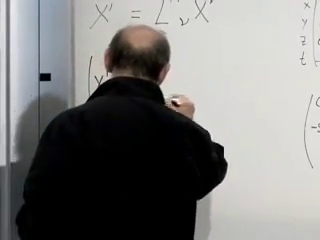
\includegraphics[width=0.8\textwidth]{lecture_06_figure_03.png}
\caption{逆變與協變分量、度規矩陣，以及不變縮併的開頭。}
\lectureframe{00:45:00}
\end{figure}

降指標並非只是裝飾。它把洛倫茲不變範數所需的正負號收納起來：
\begin{align}
  A_\mu A^\mu
  &=-(A^1)^2-(A^2)^2-(A^3)^2+(A^0)^2,                    \label{eq:l6-norm}\\
  X_\mu X^\mu
  &=t^2-x^2-y^2-z^2.
\end{align}
第二個式子是從原點到該事件的不變時空間隔。由於\(A^\mu\)和\(X^\mu\)的變換方式相同，它們的縮併也具有相同的不變性。

這種記法也帶出一條實用的記帳規則：重複的求和指標，一次寫在上方、一次寫在下方。例如：
\begin{equation}
  A_\mu A^\mu
  =\eta_{\mu\nu}A^\mu A^\nu.
\end{equation}
求和指標又稱啞指標，其名稱可以更改，而不影響所代表的量。

\begin{classroomqa}
\audiencequestion{其中一個向量是否應視為行向量，另一個視為列向量？它們的順序有影響嗎？}
\lecturerresponse{就目前的計算而言，把帶指標的量視為分量，並讓度規完成縮併即可；不必把討論轉成行與列的算符代數。這些量都是普通數，因此順序不影響結果。非對易算符則需要更仔細處理，但這不是此處討論的主題。}
\end{classroomqa}

同樣的構造也能定義兩個不同四維向量的內積：
\begin{equation}
  A\mathbin{\cdot}B=A_\mu B^\mu=A^\mu B_\mu.
\end{equation}
不必寫出明確的洛倫茲矩陣，就能看出它的不變性。由於\(A+B\)和\(A-B\)都是四維向量，它們的範數平方都是不變量：
\begin{align}
  (A+B)^2&=A^2+B^2+2A\mathbin{\cdot}B,\\
  (A-B)^2&=A^2+B^2-2A\mathbin{\cdot}B.
\end{align}
兩式相減可得
\begin{equation}
  (A+B)^2-(A-B)^2=4A\mathbin{\cdot}B,                    \label{eq:l6-polarization}
\end{equation}
因此\(A\mathbin{\cdot}B\)也是不變量。展開後即可直接得到因子 4。\editorialnote{黑板上的論證給出了這個極化恆等式；寫出因子 4，可以清楚交代口頭推導中的消去過程。}

\begin{figure}[H]
\centering
\includegraphics[width=0.8\textwidth]{lecture_06_figure_04.png}
\caption{用來分離不同四維向量內積的兩個不變平方。}
\lectureframe{00:52:20}
\end{figure}

不變量是構成物理定律的自然要素：不同於單獨的分量，它們在不同參考系中具有相同的值。

\section{固有速度與四維動量}

考慮粒子世界線上兩個相鄰的事件。它們之間的間隔是無窮小四維向量：
\begin{equation}
  dX^\mu=(dx,dy,dz,dt).
\end{equation}
對於類時世界線，固有時間定義為
\begin{equation}
  d\tau^2=dX_\mu dX^\mu
  =dt^2-dx^2-dy^2-dz^2.                                  \label{eq:l6-proper-time}
\end{equation}
固有四維速度為
\begin{equation}
  U^\mu=\frac{dX^\mu}{d\tau}.                            \label{eq:l6-four-velocity}
\end{equation}
它衡量時空位置相對於粒子自身固有時間的變化率，而不是相對於某個選定參考系的座標時間。

雖然\(U^\mu\)有四個分量，但只有三個彼此獨立。將式~\eqref{eq:l6-proper-time}除以\(d\tau^2\)可得
\begin{equation}
  U_\mu U^\mu=1.
\end{equation}
因此，四維速度是單位類時向量。選擇指向未來的方向，就確定了它的時間分量符號。

\begin{classroomqa}
\audiencequestion{當速度遠小於\(c\)時，四維速度會趨近普通速度嗎？}
\lecturerresponse{它的三個空間分量會趨近普通速度，而時間分量在\(c=1\)單位制下趨近於 1。這個關係可由鏈鎖律並計算\(dt/d\tau\)得到。}
\end{classroomqa}

對每個空間分量，
\begin{equation}
  U^i=\frac{dx^i}{d\tau}
     =\frac{dx^i}{dt}\frac{dt}{d\tau}
     =v^i\frac{dt}{d\tau}.
\end{equation}
將式~\eqref{eq:l6-proper-time}除以\(dt^2\)：
\begin{equation}
  \left(\frac{d\tau}{dt}\right)^2
  =1-v_x^2-v_y^2-v_z^2
  =1-\boldsymbol v^2.
\end{equation}
因此
\begin{equation}
  \frac{dt}{d\tau}=\frac{1}{\sqrt{1-\boldsymbol v^2}}
  =\gamma(\lvert\boldsymbol v\rvert),
\end{equation}
並且
\begin{equation}
  U^\mu=(\gamma v_x,\gamma v_y,\gamma v_z,\gamma).
                                                                  \label{eq:l6-u-components}
\end{equation}

\begin{figure}[H]
\centering
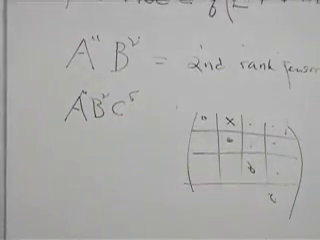
\includegraphics[width=0.8\textwidth]{lecture_06_figure_05.png}
\caption{透過固有時間計算得到\(dt/d\tau=\gamma\)，並建立固有速度與普通速度之間的關係。}
\lectureframe{01:02:00}
\end{figure}

\begin{classroomqa}
\audiencequestion{\(dx^2/dt^2\)是指二階導數嗎？向量平方是否應該產生交叉項？}
\lecturerresponse{這裡指的是\((dx/dt)^2\)，也就是一階導數的平方。此外，\(\boldsymbol v^2\)表示歐幾里得內積\(v_x^2+v_y^2+v_z^2\)，而不是形式上的和\(v_x+v_y+v_z\)的平方，所以不會有交叉項。}
\end{classroomqa}

\begin{classroomqa}
\audiencequestion{\(\gamma(v)\)中的\(v\)，是兩個座標參考系之間的相對速度，還是粒子的速度？}
\lecturerresponse{這裡指粒子在所選參考系中的速度。函數\(\gamma(v)=1/\sqrt{1-v^2}\)可以用於任意速度：在洛倫茲推進中，代入的是參考系間的相對速度；在四維速度中，代入的則是粒子速度。}
\end{classroomqa}

當\(v\ll1\)時，\(\gamma\simeq1\)，因此\(U^\mu\)的空間分量會趨近\(\boldsymbol v\)，而\(U^0\)會趨近於 1。普通速度趨近光速時，\(\gamma\)會無界增大，四維速度所有非零分量也都會無界增大。

\begin{classroomqa}
\audiencequestion{\(U^0\)的量綱不是應該是速度嗎？為什麼它會接近數值 1？}
\lecturerresponse{把\(c\)設為 1 時，量綱就被省略了。若採用\(X^0=ct\)，則
\(U^\mu=(\gamma\boldsymbol v,\gamma c)\)，所以時間分量會趨近\(c\)，而且\(U_\mu U^\mu=c^2\)。}
\end{classroomqa}

對靜止質量為\(m\)的粒子，四維動量定義為
\begin{equation}
  P^\mu=mU^\mu.
\end{equation}
在自然單位制下，
\begin{equation}
  P^\mu=(\gamma m\boldsymbol v,\gamma m).
\end{equation}
低速時，前三個分量會趨近牛頓力學中的動量\(m\boldsymbol v\)。恢復單位後可得
\begin{equation}
  P^\mu=(\gamma m\boldsymbol v,E/c),
  \qquad E=\gamma mc^2,
\end{equation}
因此
\begin{equation}
  E=mc^2+\frac{1}{2}m\boldsymbol v^2+O(mv^4/c^2).
\end{equation}
時間分量以\(c=1\)為單位表示能量；若四個分量都以動量為單位，則時間分量是能量除以\(c\)。

\begin{classroomqa}
\audiencequestion{在普通\(\boldsymbol v\)後面加上一個第四分量，所得的量本身是四維向量嗎？}
\lecturerresponse{不是。普通三維速度的變換方式並非四維向量的變換方式。因子\(\gamma\)和固有時間的定義不可或缺；四維向量是\(U^\mu\)，不是\(\boldsymbol v\)。}
\end{classroomqa}

\section{為何電場與磁場必須彼此混合}

現在我們暫時離開相對論一下。從愛因斯坦之前的運動方程出發，看看要讓它適用於所有慣性參考系，必須如何重新整理。普通加速度是普通速度對時間的導數。它在四維時空中的對應量自然是
\begin{equation}
  A^\mu=\frac{dU^\mu}{d\tau}.
\end{equation}
低速時，它的空間分量會趨近普通加速度。完整的相對論方程稍後再談；我們先看看舊的力定律。

電荷\(q\)處於電場和磁場中時，
\begin{equation}
  \boldsymbol F=m\boldsymbol a
  =q\left(\boldsymbol E+\boldsymbol v\times\boldsymbol B\right).
                                                                  \label{eq:l6-lorentz-force}
\end{equation}
電場項與粒子速度無關，磁場項則與粒子速度有關。

\begin{figure}[H]
\centering
\includegraphics[width=0.8\textwidth]{lecture_06_figure_06.png}
\caption{促使我們將\(\boldsymbol E\)與\(\boldsymbol B\)合併考慮的前相對論洛倫茲力定律。}
\lectureframe{01:18:20}
\end{figure}

假設某位觀察者看不到電場，卻看到磁場和一個運動中的電荷。電荷會受到磁力。然而，在電荷的瞬時靜止參考系中，\(\boldsymbol v=0\)，因此式~\eqref{eq:l6-lorentz-force}中的磁場項便消失。座標改變不會使實際的世界線變成慣性運動；因此新參考系中的力必須包含電場的貢獻。更精確地說，非零的四維加速度不可能只靠轉換慣性參考系就變為零，即使三維加速度及其分量確實會隨參考系而變。\editorialnote{四維加速度的這項陳述是不變的課堂論證形式，也避免把普通三維加速度本身誤當成參考系不變量。}

因此，電場和磁場必須彼此轉換。兩者合計有六個分量，所以它們既不是單一標量，也不是單一四維向量。我們需要一種新的變換對象。

\section{張量：每個指標各對應一次變換}

標量可視為零階張量，沒有指標。四維向量是階數為一的張量，帶有一個可取四種值的指標。最簡單的二階例子是兩個向量的乘積：
\begin{equation}
  A^\mu B^\nu.
\end{equation}
每個指標有四種可能，因此這個對象有\(4^2=16\)個分量，可以排成\(4\times4\)陣列。三個向量的乘積
\begin{equation}
  A^\mu B^\nu C^\sigma,
\end{equation}
有\(4^3=64\)個分量，是三階張量。更高階張量也依此類推。名稱不如定義對象的規則重要。

若
\begin{equation}
  A'^{\mu}=\Lambda^\mu{}_{\nu}A^\nu,
  \qquad
  B'^{\sigma}=\Lambda^\sigma{}_{\tau}B^\tau,
\end{equation}
則兩者的乘積會按下式變換：
\begin{equation}
  A'^{\mu}B'^{\sigma}
  =\Lambda^\mu{}_{\nu}\Lambda^\sigma{}_{\tau}
   A^\nu B^\tau.
\end{equation}
這就是逆變二階張量的定義變換律：
\begin{equation}
  T'^{\mu\sigma}
  =\Lambda^\mu{}_{\nu}\Lambda^\sigma{}_{\tau}T^{\nu\tau}.
                                                                  \label{eq:l6-tensor-transform}
\end{equation}
每個指標各對應一個洛倫茲矩陣。重複的\(\nu\)和\(\tau\)要對其求和；未縮併的\(\mu\)和\(\sigma\)則標示在帶撇參考系中所求的分量。

\begin{figure}[H]
\centering
\includegraphics[width=0.82\textwidth]{lecture_06_figure_07.png}
\caption{兩個向量的變換方式，以及由此得到的二階張量雙矩陣變換律。}
\lectureframe{01:27:15}
\end{figure}

張量不一定是單一的向量乘積。\(A^\mu B^\nu\)和\(A^\nu B^\mu\)都遵守張量變換律，它們的和，以及像下式這樣的和也一樣：
\begin{equation}
  A^\mu B^\nu+C^\mu D^\nu.
\end{equation}
張量的定義是其變換律，而非某種特定的因式分解。三階張量會多出第三個洛倫茲矩陣，依此類推。

\section{對稱張量與反對稱張量}

有兩類二階張量特別有用。對稱張量滿足
\begin{equation}
  T^{\mu\nu}=T^{\nu\mu},
\end{equation}
也就是說，對角線兩側互為鏡像的矩陣元相等。四個對角矩陣元，加上對角線一側的六個矩陣元，即可決定其餘部分，因此共有
\begin{equation}
  4+6=10
\end{equation}
個獨立分量。

反對稱張量滿足
\begin{equation}
  T^{\mu\nu}=-T^{\nu\mu}.                                \label{eq:l6-antisymmetry}
\end{equation}
在式~\eqref{eq:l6-antisymmetry}中令\(\mu=\nu\)，可得
\(T^{\mu\mu}=-T^{\mu\mu}\)，因此所有對角矩陣元都為零。三角形一側的六個矩陣元，決定另一側對應的六個矩陣元，符號則相反。因此恰有六個獨立分量。

\begin{figure}[H]
\centering
\includegraphics[width=0.82\textwidth]{lecture_06_figure_08.png}
\caption{完整的反對稱\(4\times4\)陣列：對角線上的元素為零，對角線兩側的元素符號相反。}
\lectureframe{01:34:25}
\end{figure}

這個數目正是線索。三個電場分量和三個磁場分量，恰好可以放進一個反對稱二階張量。

\section{電磁場張量}

令時空指標依照\((1,2,3,0)=(x,y,z,t)\)的順序排列在各列與各行。黑板上的排列方式是
\begin{equation}
  F_{\mu\nu}=
  \begin{pmatrix}
    0    & -B_3 & B_2  & E_1\\
    B_3  & 0    & -B_1 & E_2\\
    -B_2 & B_1  & 0    & E_3\\
    -E_1 & -E_2 & -E_3 & 0
  \end{pmatrix}.                                         \label{eq:l6-field-tensor}
\end{equation}
純空間部分的矩陣元包含磁場；一個空間指標搭配一個時間指標的矩陣元則包含電場。知道上三角部分後，便可由反對稱性得出下三角部分。

\begin{classroomqa}
\audiencequestion{磁場的矩陣元是否全為負號？這些指標是否對應於\(x,y,z\)？}
\lecturerresponse{上三角空間部分的符號交替如下：\(-B_3,+B_2,-B_1\)。指標\(1,2,3\)對應於\(x,y,z\)，而\(0\)代表時間。沿對角線反射時，每個符號都會反轉。}
\end{classroomqa}

\begin{figure}[H]
\centering
\includegraphics[width=0.82\textwidth]{lecture_06_figure_09.png}
\caption{依照這堂課中空間分量優先的順序排列的完整電磁場張量。}
\lectureframe{01:41:05}
\end{figure}

慣例上，這個張量記為\(F_{\mu\nu}\)，而非一般的\(T_{\mu\nu}\)。講師猜測這個字母可能代表法拉第，但也明確表示自己不知道這個記號的歷史。此處重要的是它的反對稱性和六個場分量，而不是對字母來源的猜測。

\begin{classroomqa}
\audiencequestion{矩陣中的每個元素，是否代表該座標平面上的場強？}
\lecturerresponse{每個元素都是電磁場張量的一個分量。含有時間指標的元素代表電場分量，而空間--空間元素則編碼磁場分量。}
\end{classroomqa}

將含時間指標的那一列和那一行分隔出來。剩下的\(3\times3\)反對稱區塊代表磁場。它的獨立分量可以用循環方式記憶：
\begin{equation}
  F_{12}=-B_3,
  \qquad F_{23}=-B_1,
  \qquad F_{31}=-B_2.                                   \label{eq:l6-magnetic-cycle}
\end{equation}
從第一個關係式開始，讓各指標依\(1\to2\to3\to1\)的順序循環。等價地，
\begin{equation}
  F_{ij}=-\epsilon_{ijk}B_k,
\end{equation}
其中\(\epsilon_{123}=+1\)。\editorialnote{Levi--Civita 公式是循環規則的標準簡潔寫法；這條規則已在黑板上逐項推導。}

\begin{figure}[H]
\centering
\includegraphics[width=0.82\textwidth]{lecture_06_figure_10.png}
\caption{反對稱張量中編碼磁場的循環空間分量。}
\lectureframe{01:46:20}
\end{figure}

電場的對應關係更直接：
\begin{equation}
  E_1=F_{10},
  \qquad E_2=F_{20},
  \qquad E_3=F_{30}.
\end{equation}

因此，磁場有兩種有用的表示方式。在三維空間中，三分量的軸向量可以和一個\(3\times3\)反對稱張量相互對應。然而在時空中，磁場只是六分量張量\(F_{\mu\nu}\)的空間部分。這種對應方式是三維空間所特有的：一個反對稱的\(4\times4\)張量有六個獨立分量，無法等同於四維向量。\editorialnote{在正旋轉下，磁場的變換方式如同向量；在反射下，更精確地說，它是軸向量，也就是偽向量。}

這項建構的目的並非只為了計算分量數目。由於\(F_{\mu\nu}\)依張量的方式變換，洛倫茲推進會自動混合其中的電場分量與磁場分量。下一講會將它與四維速度和四維加速度結合，以協變運動方程取代式~\eqref{eq:l6-lorentz-force}。

\section{關於愛因斯坦與閔可夫斯基的問題}

最後幾分鐘的討論從形式體系轉向它的歷史起源。講者以回憶而非定論的方式回答；這項限定也是這段問答的一部分。

\begin{classroomqa}
\audiencequestion{愛因斯坦是基於概念上的理由尋求洛倫茲不變的表述，還是受到特定觀測結果的驅使？}
\lecturerresponse{自然定律在所有慣性參考系中都應具有相同形式，這項原理是他推理的核心。當時也有關於光的實驗證據，以及未能探測到相對於以太運動的結果；不過講師明確表示，他不確定愛因斯坦當時知道哪些結果，也不確定這些結果對他的影響有多大。概念上的要求是，麥克斯韋方程組與洛倫茲力都應遵守相對性原理，而這要求電場、磁場和速度分量一起變換。}
\end{classroomqa}

愛因斯坦在1905年的論述沒有使用此處採用的簡潔四維向量記法，而是逐一處理各分量，並明確寫出所需的\(\gamma\)因子和速度。之後，閔可夫斯基以幾何方式將同樣的結構整理成四維時空。

\begin{classroomqa}
\audiencequestion{愛因斯坦是否抗拒閔可夫斯基的時空表述？閔可夫斯基又是在多久之後提出這種表述？}
\lecturerresponse{課堂上講者的回憶是，愛因斯坦起初不太接受四維幾何的說法，但很快便認同它的價值。講者暫且估計，這大約是在1905年的論文之後兩年，也許是1907年；他強調自己是在回憶，而非確定歷史事實。}
\end{classroomqa}

\begin{classroomqa}
\audiencequestion{閔可夫斯基是數學家還是物理學家？他還有哪些貢獻？他是否受到洛倫茲或菲茨傑拉德的影響？}
\lecturerresponse{講者沒有聲稱自己能給出確定答案。數學家和物理學家的區別沒有進一步討論；一位聽眾提出更正，打斷了講者對閔可夫斯基其他工作的概略評論；至於可能的影響來源，講者也明確表示尚不確定。就這段討論而言，可以確定的是，閔可夫斯基以四維幾何記法，對相對論作了關鍵性的整理。}
\end{classroomqa}

\begin{classroomqa}
\audiencequestion{混合\(\boldsymbol E\)與\(\boldsymbol B\)的變換，在愛因斯坦1905年的工作中就已經出現了嗎？}
\lecturerresponse{有，但當時是逐一寫出各分量，而不是寫成單一的場張量方程。課堂上拿麥克斯韋的分量方程作比較：在能揭示共同結構的簡潔記法出現之前，相關內容就已經存在。閔可夫斯基的貢獻，是用時空語言有系統地呈現這個結構。}
\end{classroomqa}

這讓我們回到一開始提出的數學要點。分量對於計算不可或缺，但唯有將它們理解為同一個會變換的物件之組成部分，定律才變得清晰易懂。接下來要做的是利用\(F_{\mu\nu}\)，將帶電粒子的運動方程寫成在所有慣性系中形式皆相同的樣子。
\chapter{帶電粒子、場的變換與相對論性波動}

上次我們開始探討：在相對論原理的限制下，帶電粒子如何在電場和磁場中運動。熟悉的洛倫茲力定律已經透露了線索：磁力項取決於粒子的速度，因此不同觀測者無法各自對電場與磁場的區分達成一致。我們的任務是重新表述這條定律，使所有慣性觀測者使用的方程形式相同，儘管場和粒子的速度會隨參考系而改變。

除非另有說明，我們採用\(c=1\)的單位制，度規號差為\((-,-,-,+)\)。時空分量依照空間分量在前的順序排列：
\begin{equation}
  \mu=(1,2,3,0)=(x,y,z,t).
\end{equation}
拉丁指標\(m,n\)只取三個空間方向。

\section{牛頓力定律中能保留下來的部分}

在牛頓力學中，
\begin{equation}
  \boldsymbol F=m\boldsymbol a
\end{equation}
在每個慣性系中形式都相同，因為伽利略觀測者對加速度的判定一致。他們對粒子的質量和所受的力也有相同的判定。運動學一旦改變，就沒有理由預期力與普通加速度之間的這種特定關係仍會原封不動地成立。

電磁學和引力已經提醒我們，相對論性的推廣不必彼此相似。庫侖定律和牛頓萬有引力定律都是平方反比定律，但若不更深入地改變時空幾何，引力就無法自然地納入狹義相對論。電磁學則可以。事實上，磁性本身就是一種相對論效應：恢復\(c\)的因子後，磁力項會帶有速度除以\(c\)的因子，並在形式極限\(c\to\infty\)下消失。

牛頓定律中能持續保留下來的，是力等於動量的變化率這項陳述。對於靜止質量不變的粒子，
\begin{equation}
  \boldsymbol F
  =m\frac{d\boldsymbol v}{dt}
  =\frac{d}{dt}(m\boldsymbol v)
  =\frac{d\boldsymbol p}{dt}.
\end{equation}
相對論會改變動量與速度之間的關係，但會保留這種組織方程的方式。

\begin{figure}[H]
\centering
\includegraphics[width=0.64\textwidth]{lecture_07_figure_01.png}
\caption{黑板上正在將力改寫為\(d\boldsymbol p/dt\)，同時寫出洛倫茲定律中的電場項。}
\lectureframe{00:08:20}
\end{figure}

在\(c=1\)的單位制下，前相對論形式的洛倫茲力定律為
\begin{equation}
  \frac{d\boldsymbol p}{dt}
  =q\bigl(\boldsymbol E+\boldsymbol v\times\boldsymbol B\bigr).
  \label{eq:lorentz-three}
\end{equation}
電場和磁場都可能依賴位置與時間。現在的非相對論極限是\(v\ll 1\)，而不是數值常數\(c=1\)以某種方式改變的極限。\eqref{eq:lorentz-three}中的電場項已經是普通向量。若要把磁力項寫成能帶入時空的形式，我們就必須重新檢視叉積。

\section{以反對稱張量表示叉積}

取兩個三維向量\(\boldsymbol A\)和\(\boldsymbol B\)。它們的外積
\begin{equation}
  T_{mn}=A_mB_n
\end{equation}
是具有九個分量的二階張量，一般而言沒有對稱性。將它反對稱化後，得到
\begin{equation}
  K_{mn}=A_mB_n-A_nB_m,
  \qquad K_{mn}=-K_{nm}.
  \label{eq:antisym-product}
\end{equation}
對角元為零，而對角線以下的每個元素都由其上方對應的元素決定。因此，\(3\times3\)反對稱張量只有三個獨立分量。

這個數目很有啟發性，但光靠它還不足以得出結論。三個量不會自動依照向量的方式變換。不過在三維中，\eqref{eq:antisym-product}的三個獨立元素可以對應到叉積\(\boldsymbol C=\boldsymbol A\times\boldsymbol B\)的分量。黑板上先暫時把\(C_2\)放在右上方：

\begin{figure}[H]
\centering
\includegraphics[width=0.75\textwidth]{lecture_07_figure_02.png}
\caption{反對稱乘積的三個獨立元素，正逐一對應到\(\boldsymbol C\)的分量。此處右上方的標記仍是暫定的。}
\lectureframe{00:17:33}
\end{figure}

依序輪換\(1\to2\to3\to1\)，可得分量公式
\begin{align}
  C_3 &= A_1B_2-A_2B_1, \\
  C_1 &= A_2B_3-A_3B_2, \\
  C_2 &= A_3B_1-A_1B_3.
  \label{eq:cross-components}
\end{align}
最後一行顯示，右上方的元素是\(-C_2\)，而不是\(C_2\)。這項修正是論證的一部分，不應當作細節略過。

\begin{figure}[H]
\centering
\includegraphics[width=0.62\textwidth]{lecture_07_figure_03.png}
\caption{完整的循環分量恆等式，確定了反對稱陣列中的暫定符號。}
\lectureframe{00:21:54}
\end{figure}

因此得到的矩陣為
\begin{equation}
  K_{mn}=
  \begin{pmatrix}
    0 & C_3 & -C_2 \\
    -C_3 & 0 & C_1 \\
    C_2 & -C_1 & 0
  \end{pmatrix}.
  \label{eq:cross-matrix}
\end{equation}

這種記號背後有一個實用的幾何圖像。指標為\(1,2\)的分量自然屬於\(xy\)平面，並對應到沿垂直的\(z\)軸方向的向量分量。同一個有向物件可以用平面表示，也可以用垂直於該平面的箭頭表示。箭頭的描述只適用於三維；在更高維中，反對稱二階張量依然存在，但其分量數不再等於向量的分量數。因此，能夠推廣叉積的是張量，而不是垂直箭頭。

等價地，選定一種定向後，
\begin{equation}
  C_k=\frac12\epsilon_{kmn}K_{mn}.
\end{equation}
必須選定定向，這正是右手定則，以及極向量與軸向量之間熟悉區別的由來。
\editorialnote{Levi--Civita 公式與軸向量一詞，是表述講課中明確闡述的平面與法向量幾何的標準記號。}

\section{磁場的張量形式}

磁場也可以採用同樣的對偶描述。我們將其反對稱空間張量定義為
\begin{equation}
  B_{mn}=
  \begin{pmatrix}
    0 & -B_3 & B_2 \\
    B_3 & 0 & -B_1 \\
    -B_2 & B_1 & 0
  \end{pmatrix}.
  \label{eq:magnetic-tensor}
\end{equation}
相較於\eqref{eq:cross-matrix}，此處多出的整體負號是一種約定。約定一旦選定，就必須前後一致；若將向量的三個分量全部變號，表示的是採用相反定向約定時，同一種由張量對應到向量的方式。

\begin{figure}[H]
\centering
\includegraphics[width=0.72\textwidth]{lecture_07_figure_04.png}
\caption{磁場既以反對稱空間陣列表示，也以其三個向量分量表示。}
\lectureframe{00:24:40}
\end{figure}

現在取叉積的第三個分量：
\begin{align}
  (\boldsymbol v\times\boldsymbol B)_3
  &=v_1B_2-v_2B_1 \\
  &=v_1B_{13}+v_2B_{23}+v_3B_{33}.
\end{align}
可以加上最後一項，因為\(B_{33}=0\)。輪換自由分量後，可得簡潔的規則
\begin{equation}
  (\boldsymbol v\times\boldsymbol B)_m=v_nB_{nm},
  \label{eq:cross-contraction}
\end{equation}
其中重複指標\(n\)依愛因斯坦求和約定加總。因此，磁力為
\begin{equation}
  F_m^{(B)}=qv_nB_{nm}.
\end{equation}

\begin{figure}[H]
\centering
\includegraphics[width=0.78\textwidth]{lecture_07_figure_05.png}
\caption{\(\boldsymbol v\times\boldsymbol B\)的第三個分量，以及它以\(B_{nm}\)縮併表示的一般形式。}
\lectureframe{00:28:30}
\end{figure}

\begin{classroomqa}
\audiencequestion{自由指標\(m\)是否標記力的某個磁力分量？}
\lecturerresponse{不是。它標記的是正在計算的那個力的空間分量。目前的論證只是把電場設為零，而此處每個指標都只取三個空間方向。}
\end{classroomqa}

張量記號讓磁場不做功這項性質幾乎可直接看出。對速率平方微分：
\begin{align}
  \frac{d}{dt}(v_mv_m)
  &=2\dot v_m v_m \\
  &\propto 2(\boldsymbol v\times\boldsymbol B)_m v_m \\
  &=2v_nB_{nm}v_m.
  \label{eq:speed-derivative}
\end{align}
含有\(m=n\)的項會消失，因為\(B_{nm}\)的對角元為零。每個非對角項都與另一項成對，兩項中的\(m\)和\(n\)互換；由於\(v_nv_m\)是對稱的，而\(B_{nm}\)是反對稱的，兩項便互相抵消。
因此
\begin{equation}
  \frac{d}{dt}(v_mv_m)=0.
\end{equation}
純磁力會使軌跡彎曲，卻不改變粒子的速率或動能。

\begin{figure}[H]
\centering
\includegraphics[width=0.68\textwidth]{lecture_07_figure_06.png}
\caption{\(v_nB_{nm}v_m\)中的配對項會互相抵消，因為磁張量的指標互換時，符號會改變。}
\lectureframe{00:35:40}
\end{figure}

這個證明刻意比「叉積垂直於它的第一個因子」這種說法更繁複。後者只適用於三維向量表示。真正能延伸到四維的論證，是對稱二階張量與反對稱張量的縮併為零。

\begin{classroomqa}
\audiencequestion{磁場必須與時間無關，速率才會保持不變嗎？}
\lecturerresponse{上面的代數推導從未對磁場微分，因此不要求\(\partial_t\boldsymbol B=0\)。單獨的磁力項仍然不做功。不過在電動力學中，變化的磁場會產生電場，而電場可以改變粒子的速率。}
\end{classroomqa}

\section{電場與磁場為何必須混合}

無須進行任何四維計算，就能看出\(\boldsymbol E\)與\(\boldsymbol B\)會混合。考慮低速運動，此時對加速度使用普通的牛頓力學描述已經足夠。設磁場沿\(y\)軸，帶電粒子沿\(x\)軸運動。磁力則沿\(z\)軸：
\begin{equation}
  \boldsymbol F=q\boldsymbol v\times\boldsymbol B.
\end{equation}

\begin{figure}[H]
\centering
\includegraphics[width=0.62\textwidth]{lecture_07_figure_07.png}
\caption{粒子橫越磁場運動的黑板示意圖；圖中的三個方向用來比較實驗室系與共動系的描述。}
\lectureframe{00:42:20}
\end{figure}

不用教室裡的透視畫法，也可以重新畫出這個幾何關係：
\begin{figure}[H]
\centering
\begin{tikzpicture}[scale=1.05,>=Stealth]
  \draw[->] (0,0) -- (3.8,0) node[right] {\(x\)};
  \draw[->] (0,0) -- (-1.9,2.4) node[above left] {\(y\)};
  \draw[->] (0,0) -- (0,3.1) node[above] {\(z\)};
  \draw[->,very thick] (0,0) -- (2.7,0)
    node[midway,below] {\(\boldsymbol v\)};
  \draw[->,very thick] (0,0) -- (-1.35,1.7)
    node[midway,above left] {\(\boldsymbol B\)};
  \draw[->,very thick] (0,0) -- (0,2.35)
    node[midway,right] {\(\boldsymbol F,\ \boldsymbol E'\)};
\end{tikzpicture}
\caption{在實驗室系中，沿\(z\)方向的力是磁力；在瞬時共動系中，同一個力必須是電力。}
\end{figure}

現在考慮一位在該瞬間與粒子一起運動的觀測者。粒子在新參考系中的速度為零，因此磁力項\(q\boldsymbol v'\times\boldsymbol B'\)消失。然而在低速極限下，兩位觀測者都必須同意粒子具有沿\(z\)方向的加速度。若洛倫茲力定律在兩個參考系中形式相同，共動觀測者就必須將這個力歸因於沿\(z\)方向的電場\(\boldsymbol E'\)。因此，在實驗室系中純為磁性的場，到了運動參考系中便不再是純磁場。

這就是我們要尋找一個其分量同時包含兩種場的物件的物理原因。參考系改變時，\(\boldsymbol E\)的三個分量和\(\boldsymbol B\)的三個分量不只是各自旋轉；兩組分量也會彼此混合。

\section{電磁場張量}

電場與磁場合計有六個分量。四維反對稱張量也有六個獨立分量，因為
\begin{equation}
  \frac{4(4-1)}{2}=6.
\end{equation}
這並不表示反對稱張量是唯一能由六個量組成的集合；六個純量，或一個向量加上兩個純量，也同樣包含六個數。反對稱張量是其分量能以所需方式混合的自然幾何物件。

為了明確呈現黑板上的約定，我們依照空間分量在前的順序\((1,2,3,0)\)，寫出逆變張量：
\begin{equation}
  F^{\mu\nu}=
  \begin{pmatrix}
    0 & -B_3 & B_2 & E_1 \\
    B_3 & 0 & -B_1 & E_2 \\
    -B_2 & B_1 & 0 & E_3 \\
    -E_1 & -E_2 & -E_3 & 0
  \end{pmatrix}.
  \label{eq:l07-field-tensor}
\end{equation}
左上角的\(3\times3\)區塊正是磁張量\eqref{eq:magnetic-tensor}；一個空間指標和一個時間指標所構成的分量則包含電場。其餘元素由反對稱性決定。

\begin{figure}[H]
\centering
\includegraphics[width=0.72\textwidth]{lecture_07_figure_08.png}
\caption{磁場的空間區塊與電場的時間—空間欄，一同組成四維場張量。}
\lectureframe{00:46:35}
\end{figure}

\begin{classroomqa}
\audiencequestion{這些場分量應該使用上標還是下標？}
\lecturerresponse{只看三個空間指標時，黑板上有時會省略上標與下標的區別，以便辨認熟悉的馬克士威--法拉第場。在協變計算中，則必須恢復這項區別：依照所選的度規約定，升高或降低空間指標會改變符號。}
\end{classroomqa}

不變的不是黑板上某種特定的符號排列，而是反對稱時空張量，以及一套前後一致的度規與指標約定。記號\(F\)可能讓人聯想到法拉第，不過本講並未有把握地宣稱這項歷史歸屬。愛因斯坦在1905年推導出電場與磁場分量的變換；簡潔的四維張量語言則隨後來與閔可夫斯基相關的時空表述而出現。

\section{四維速度與四維力}

方程中描述粒子的部分也必須寫成協變形式。固有時\(\tau\)是不變量，因此以固有時對位置四維向量微分，會得到另一個四維向量：
\begin{equation}
  u^\mu=\frac{dx^\mu}{d\tau}
  =\gamma(v_x,v_y,v_z,1),
  \qquad
  \gamma=\frac{1}{\sqrt{1-v^2}}.
  \label{eq:four-velocity}
\end{equation}
最後一個分量由\(dt/d\tau=\gamma\)得出。四維動量為
\begin{equation}
  p^\mu=mu^\mu,
\end{equation}
其空間部分就是相對論動量
\(\boldsymbol p=m\gamma\boldsymbol v\)。

\begin{figure}[H]
\centering
\includegraphics[width=0.75\textwidth]{lecture_07_figure_09.png}
\caption{四維速度及其分量、洛倫茲因子與四維動量。}
\lectureframe{00:50:30}
\end{figure}

由於\(p^\mu\)是四維向量，而\(\tau\)是純量，相對論中自然的方程左側為
\begin{equation}
  f^\mu\equiv\frac{dp^\mu}{d\tau}.
  \label{eq:four-force-def}
\end{equation}
四維力不能任意選取。四維速度的模固定為
\begin{equation}
  u_\mu u^\mu=1.
\end{equation}
沿世界線微分可得
\begin{align}
  0
  &=\frac{d}{d\tau}(u_\mu u^\mu) \\
  &=\frac{du_\mu}{d\tau}u^\mu
    +u_\mu\frac{du^\mu}{d\tau} \\
  &=2u_\mu\frac{du^\mu}{d\tau}.
\end{align}
質量不變時，這表示
\begin{equation}
  f^\mu u_\mu=0.
  \label{eq:force-orthogonal}
\end{equation}
因此四維力與四維速度在閔可夫斯基度規下正交。這是由\(u^\mu\)的歸一化所導出的純運動學限制，並非電磁學特有的性質。

\begin{figure}[H]
\centering
\includegraphics[width=0.64\textwidth]{lecture_07_figure_10.png}
\caption{四維速度的單位模，以及由此導出的四維力與四維速度正交關係。}
\lectureframe{00:56:50}
\end{figure}

三維磁力的計算已經提供了滿足\eqref{eq:force-orthogonal}的方法。將反對稱張量與一個速度向量縮併：
\begin{equation}
  \boxed{
  \frac{dp^\mu}{d\tau}=qF^{\mu\nu}u_\nu.}
  \label{eq:covariant-lorentz}
\end{equation}
確實，
\begin{equation}
  f^\mu u_\mu
  =qF^{\mu\nu}u_\nu u_\mu=0,
\end{equation}
這是因為\(F^{\mu\nu}\)具有反對稱性，而\(u_\nu u_\mu\)具有對稱性。這不是唯一可能的相對論性力律，但它是同時對電磁場與速度呈線性的最簡單力律。

\begin{figure}[H]
\centering
\includegraphics[width=0.72\textwidth]{lecture_07_figure_11.png}
\caption{左側是協變形式的洛倫茲力方程；右側顯示它與另一個四維速度縮併後為零。}
\lectureframe{01:00:00}
\end{figure}

\section{還原為通常的洛倫茲力定律}

看起來具有協變形式的方程，仍必須重現已知的力定律。採用開頭所述的度規約定，
\begin{equation}
  u_\mu=\gamma(-v_x,-v_y,-v_z,1).
\end{equation}
考慮\(x\)分量，\eqref{eq:l07-field-tensor}與\eqref{eq:covariant-lorentz}給出
\begin{align}
  \frac{dp^1}{d\tau}
  &=q\bigl(F^{12}u_2+F^{13}u_3+F^{10}u_0\bigr) \\
  &=q\gamma\bigl(B_3v_y-B_2v_z+E_1\bigr) \\
  &=q\gamma\bigl[\boldsymbol E+\boldsymbol v\times
    \boldsymbol B\bigr]_x.
  \label{eq:x-force}
\end{align}
其餘空間分量只要循環置換指標即可得到。

\begin{classroomqa}
\audiencequestion{分量展開中的\(qE_x\)項在哪裡？}
\lecturerresponse{它就是\(qF^{10}u_0\)這一項。含有一個空間指標與一個時間指標的場張量分量，代表電場分量，而\(u_0=\gamma\)。}
\end{classroomqa}

右側的\(\gamma\)因子不是額外的力。由於
\begin{equation}
  \frac{dp^i}{d\tau}=\frac{dt}{d\tau}\frac{dp^i}{dt}
  =\gamma\frac{dp^i}{dt},
\end{equation}
它會從\eqref{eq:x-force}的兩側約去。因此，精確的空間方程仍然是
\begin{equation}
  \frac{d\boldsymbol p}{dt}
  =q\bigl(\boldsymbol E+\boldsymbol v\times\boldsymbol B\bigr),
  \qquad
  \boldsymbol p=m\gamma\boldsymbol v.
  \label{eq:exact-three-force}
\end{equation}
熟悉的形式保留下來，相對論效應則包含在動量之中。

\begin{figure}[H]
\centering
\includegraphics[width=0.75\textwidth]{lecture_07_figure_12.png}
\caption{約去共同的固有時因子後，便還原為三維洛倫茲力定律；動量仍帶有\(\gamma\)因子。}
\lectureframe{01:06:30}
\end{figure}

時間分量則給出相應的能量關係，
\begin{equation}
  \frac{dp^0}{dt}=q\boldsymbol E\cdot\boldsymbol v,
\end{equation}
因此磁場不做功，而電場可能改變粒子的能量。
\editorialnote{時間分量的檢驗直接對應到講課中的空間分量計算；列出這項檢驗，是為了以四維記號呈現同樣的不做功性質。}

\begin{classroomqa}
\audiencequestion{這個推導屬於數學還是物理？}
\lecturerresponse{兩者皆是。張量代數提供了簡潔的形式，但其中也包含重要的物理內容：所有慣性系都遵守相同定律的原理，以及運動方程為二階方程的假設。二階定律根據位置與速度預測未來；三階定律則需要把加速度也列為額外的初始資料。自然界採用哪一種定律，取決於實驗，而不是記號。}
\end{classroomqa}

\section{場的變換方式}

方程\eqref{eq:covariant-lorentz}在每個參考系中形式都相同，因為等式兩側都是四維向量。場張量本身的變換方式是每個指標各乘上一個洛倫茲矩陣：
\begin{equation}
  F'^{\mu\nu}
  =\Lambda^\mu{}_{\rho}\Lambda^\nu{}_{\sigma}F^{\rho\sigma}.
  \label{eq:tensor-transform}
\end{equation}
黑板上先從變換簡單乘積\(A^\mu B^\nu\)推導這條規則。一旦知道向量乘積如何變換，再利用線性性，就能得到任意二階張量的變換規則。

沿\(1\)軸的推動，其座標變換為
\begin{align}
  x'^1&=\gamma(x^1-vx^0), &
  x'^0&=\gamma(x^0-vx^1), \\
  x'^2&=x^2, & x'^3&=x^3.
\end{align}
對張量的兩個指標分別施加相同的變換。對於平行於推動方向的分量，黑板上先從一個乘積開始：
\begin{align}
  (A'^0B'^1)
  =\gamma^2\bigl(
     A^0B^1-vA^0B^0-vA^1B^1+v^2A^1B^0
   \bigr).
\end{align}
將各個乘積換成相應的張量分量，再利用反對稱性\(F^{00}=F^{11}=0\)和\(F^{10}=-F^{01}\)，可得
\begin{equation}
  F'^{01}
  =\gamma^2(1-v^2)F^{01}
  =F^{01}.
\end{equation}
因此，平行於運動方向的電場分量不變。平行的磁場分量也有類似的行為。

橫向分量則不同。按照黑板上帶撇參考系與符號的約定，
\begin{align}
  F'^{02}
  &=\gamma\bigl(F^{02}-vF^{12}\bigr), \\
  E'_2
  &=\gamma(E_2+vB_3).
  \label{eq:e-transform}
\end{align}
橫向電場分量會包含一部分磁場分量的貢獻。其餘變換定律可依照同一套雙指標規則推導，講課中將它們留作練習。

\begin{figure}[H]
\centering
\includegraphics[width=0.76\textwidth]{lecture_07_figure_13.png}
\caption{橫向張量變換式中，\(E'_2\)分量包含一項正比於\(vB_3\)。}
\lectureframe{01:23:40}
\end{figure}

\eqref{eq:e-transform}中的符號取決於哪個參考系被視為以\(+v\)運動，也取決於指標與度規的約定。不受這些選擇影響的是：橫向電場與磁場分量會彼此混合，而變換後的協變力方程依然成立。

\begin{classroomqa}
\audiencequestion{對於導線中的電流，有沒有某個運動速度能讓磁場消失？}
\lecturerresponse{只跟著傳導電子一起運動並不足夠，因為在新參考系中，正電荷晶格也會運動。因此，中性載流導線的情況比單一電荷團的運動複雜。純磁場無法經由參考系變換完全消除。若電場與磁場同時存在，兩者變換後的部分在某些特殊情況下可以相消；對於單一勻速運動的電荷，電荷的靜止系就是能讓其磁場消失的簡單例子。}
\end{classroomqa}

精確的不變量判據涉及
\begin{equation}
  \boldsymbol B^2-\boldsymbol E^2,
  \qquad
  \boldsymbol E\cdot\boldsymbol B.
\end{equation}
只有電場佔主導且\(\boldsymbol E\cdot\boldsymbol B=0\)時，才可能存在滿足\(\boldsymbol B'=0\)的參考系。在某個參考系中呈現為純磁場的場是磁場佔主導，因此無法滿足這項條件。
\editorialnote{這些不變量判據精確表達了課堂討論中得出的限定條件；其推導留待之後處理。}

\begin{classroomqa}
\audiencequestion{電純量位勢和磁向量位勢會組成四維向量嗎？}
\lecturerresponse{會。依照符號約定不同，它們組合成四維位勢\(A^\mu\)。麥克斯威方程組會系統性地運用這個物件。}
\end{classroomqa}

\section{場的導數}

現在我們不再只考慮單一粒子的軌跡，而要考慮遍布時空的場。設
\begin{equation}
  \phi=\phi(x^1,x^2,x^3,x^0)
\end{equation}
它是一個純量場。這個場的四個偏導數構成四維向量的協變分量：
\begin{equation}
  \partial_\mu\phi
  \equiv\frac{\partial\phi}{\partial x^\mu}
  =\left(
    \frac{\partial\phi}{\partial x},
    \frac{\partial\phi}{\partial y},
    \frac{\partial\phi}{\partial z},
    \frac{\partial\phi}{\partial t}
  \right).
\end{equation}
對洛倫茲座標變換應用鏈鎖律，即可證明這項協變變換定律。升高指標會使空間分量變號，而時間分量的符號保持不變：
\begin{equation}
  \partial^\mu\phi
  =\left(
    -\frac{\partial\phi}{\partial x},
    -\frac{\partial\phi}{\partial y},
    -\frac{\partial\phi}{\partial z},
    \frac{\partial\phi}{\partial t}
  \right).
\end{equation}

每次微分都會引入一個下標。因此，\(\partial_\nu V^\mu\)是具有一個上標和一個下標的二階張量；對張量微分，會得到多出一個下標的物件。這是寫出不選定任何慣性系的場方程所需的基本規則。

\section{不變的純量波動方程}

最簡單的波動方程含有二階導數。若要讓方程在每個慣性系中都維持相同形式，左側就應該是純量。將導數的指標縮併，可得最簡單且唯一的選擇：
\begin{equation}
  \boxed{\partial^\mu\partial_\mu\phi=0.}
  \label{eq:wave-covariant}
\end{equation}
依照目前的度規號差，將它展開為各分量：
\begin{equation}
  \frac{\partial^2\phi}{\partial t^2}
  -\frac{\partial^2\phi}{\partial x^2}
  -\frac{\partial^2\phi}{\partial y^2}
  -\frac{\partial^2\phi}{\partial z^2}=0.
  \label{eq:wave-components}
\end{equation}
\eqref{eq:wave-covariant}中的縮併明確顯示了洛倫茲不變性；方程\eqref{eq:wave-components}則是將同一陳述逐分量寫出。

\begin{figure}[H]
\centering
\includegraphics[width=0.75\textwidth]{lecture_07_figure_14.png}
\caption{純量波動方程的導數縮併形式，以及時間項減去空間項的分量展開。}
\lectureframe{01:39:40}
\end{figure}

\begin{classroomqa}
\audiencequestion{波動方程右側一定要是零嗎？}
\lecturerresponse{不一定。右側可以是任何與問題相容的純量。以常數乘上\(\phi\)，或使用與\(\phi^2\)成正比的非線性純量函數，都仍然符合協變性。取零則得到最簡單的自由波動方程。}
\end{classroomqa}

這個純量範例是為了鋪陳後續內容。馬克斯威方程組中電場與磁場的混合更為複雜，但同樣可以寫成由指標結構直接顯示洛倫茲不變性的形式。下次我們會回到這個問題。
\chapter{度規、膨脹與初步宇宙學}

前一講結束時，我們已得到一個洛倫茲不變的波動方程，正準備把麥克斯威方程組寫成時空形式。現在，在轉向引力之前，一位聽眾的提問提醒我們：對稱性本身能決定物理理論的多少內容？答案很明確：能決定很多，但不是全部。洛倫茲不變性是篩選可能定律的有力條件，但不能取代其餘物理假設或實驗。

\section{對稱性無法決定的部分}

\begin{classroomqa}
\audiencequestion{既然已知電場和磁場會在洛倫茲變換下共同變換，麥克斯威方程組是否就能單憑相對論推出？}
\lecturerresponse{不能。相對論限制了方程的形式，但建構方程時還用到了線性、導數階數較低、場的變換方式，以及實驗資訊。缺少這些額外條件，仍然可能有許多洛倫茲協變的場方程。}
\end{classroomqa}

在開頭的討論中，最重要的額外假設是線性。若\(A(x,t)\)是某個線性場方程的解，則對任意常數\(\lambda\)，\(\lambda A(x,t)\)也會是解。若\(A\)和\(B\)都是解，則\begin{equation}
  C(x,t)=A(x,t)+B(x,t).
  \label{eq:superposition}
\end{equation}也是解。這就是疊加原理。兩列無源電磁波可以交會後各自保持原狀，不會像物質物體那樣直接碰撞。它們可以透過帶電物質間接相互作用，因為每列波都會推動電荷，而運動中的電荷會輻射；但真空場方程本身是線性的。

\begin{figure}[H]
\centering
\includegraphics[width=0.64\textwidth]{lecture_08_figure_01.png}
\caption{討論疊加原理時畫在黑板上的兩個波形。兩者相加後仍是允許的無源波。}
\lectureframe{00:05:30}
\end{figure}

諧振子讓這套代數關係一目了然。假設\begin{equation}
  m\ddot x=-kx.
  \label{eq:linear-oscillator}
\end{equation}。若\(x_1\)和\(x_2\)都滿足\eqref{eq:linear-oscillator}，則\begin{equation}
  m(\ddot x_1+\ddot x_2)
  =-k(x_1+x_2),
\end{equation}，所以\(x_1+x_2\)也是解。不過，若加入非線性項\begin{equation}
  m\ddot x=-kx+p x^2,
  \label{eq:nonlinear-oscillator}
\end{equation}，兩者之和就不再成立：\begin{equation}
  (x_1+x_2)^2=x_1^2+x_2^2+2x_1x_2.
\end{equation}。交叉項\(2x_1x_2\)在兩個各自的方程中都沒有對應項。此時，兩種運動便會互相影響。

\begin{figure}[H]
\centering
\includegraphics[width=0.73\textwidth]{lecture_08_figure_02.png}
\caption{比較兩個振子各自的方程與其和所滿足的方程。二次項顯示出額外的交叉項，因而破壞疊加原理。}
\lectureframe{00:10:10}
\end{figure}

這個例子確立了一項方法論要點，整段宇宙學討論都會沿用：對稱性告訴我們哪些量可以組合，以及哪些方程形式是允許的；動力學和觀測則告訴我們自然界採用的是哪一個允許的方程。

\section{間隔即幾何}

現在我們離開電磁學，簡要進入廣義相對論與宇宙學。起點是相鄰事件之間的間隔。以四維座標\(x^\mu\)標記一個事件，並以\(x^\mu+dx^\mu\)標記鄰近事件。在慣性笛卡兒座標中，採用\(c=1\)和\((+,-,-,-)\)的號差約定，\begin{equation}
  d\tau^2
  =dt^2-dx^2-dy^2-dz^2
  =dx^\mu dx_\mu
  =\eta_{\mu\nu}\,dx^\mu dx^\nu.
  \label{eq:minkowski-interval}
\end{equation}。不變的是\(d\tau^2\)，而不是任何單一座標差。洛倫茲變換會改變\(dt,dx,dy,dz\)，但會保留這個二次組合。因此，狹義相對論也可以理解為閔可夫斯基時空的幾何。

\begin{figure}[H]
\centering
\includegraphics[width=0.72\textwidth]{lecture_08_figure_03.png}
\caption{閔可夫斯基間隔依序以分量、縮併指標和度規張量的記號表示。}
\lectureframe{00:14:50}
\end{figure}

\eqref{eq:minkowski-interval}的簡單形式取決於座標選擇。即使是平坦平面，若座標標記得不恰當，係數也可能變得不熟悉。假設\(x\)以公分測量，而\(y\)以公尺測量。對於一個物理位移，\begin{equation}
  ds^2=dx^2+\left(\frac{dy}{100}\right)^2
      =dx^2+10^{-4}dy^2.
  \label{eq:mixed-units}
\end{equation}。因子\(10^{-4}\)與曲率無關，只是用來換算單位。

\begin{figure}[H]
\centering
\includegraphics[width=0.59\textwidth]{lecture_08_figure_04.png}
\caption{以公分標記一個軸、以公尺標記另一個軸的平坦平面。不相同的度規係數反映的是單位，而非曲率。}
\lectureframe{00:20:10}
\end{figure}

斜座標會引入混合項。在二維中，最一般的局部二次型可寫成\begin{align}
  ds^2
  &=a_{11}\,dx^2+a_{12}\,dx\,dy\notag\\
  &\quad+a_{21}\,dy\,dx+a_{22}\,dy^2,
  \qquad a_{12}=a_{21}.
  \label{eq:quadratic-form}
\end{align}。由於普通微分可以交換，\(dx\,dy=dy\,dx\)，只有係數陣列的對稱部分會有貢獻。我們把係數整理成矩陣\begin{equation}
  g=
  \begin{pmatrix}
    a_{11} & a_{12}\\
    a_{21} & a_{22}
  \end{pmatrix}.
  \label{eq:metric-matrix}
\end{equation}。這個矩陣就是\emph{度規}，它是將座標差轉換為物理間隔的局部規則。

\begin{figure}[H]
\centering
\includegraphics[width=0.71\textwidth]{lecture_08_figure_05.png}
\caption{二次微分形式，以及其對稱的\(2\times2\)係數矩陣；此處正是將該矩陣辨認為度規之時。}
\lectureframe{00:24:07}
\end{figure}

均勻的矩形或斜交網格會給出常數係數。如果座標線彎曲、逐漸密集或逐漸疏開，即使底層曲面仍然平坦，這些係數也會成為位置的函數。一般的時空記號是
\begin{equation}
  ds^2=g_{\mu\nu}(x)\,dx^\mu dx^\nu.
  \label{eq:general-metric}
\end{equation}

\begin{figure}[H]
\centering
\includegraphics[width=0.66\textwidth]{lecture_08_figure_06.png}
\caption{座標網格可以隨位置改變後的一般位置相依度規。}
\lectureframe{00:28:10}
\end{figure}

在指定的座標系中知道\(g_{\mu\nu}\)，便能確定局部距離、時間和角度，進而確定幾何。反過來則不唯一：同一幾何有無窮多種座標描述，因此也有無窮多組由座標變換彼此關聯的係數函數。

\section{座標複雜性與內在曲率}

現在必須區分複雜的度規與彎曲的空間。把一張紙捲成圓柱，不要拉伸它。紙在房間中的外觀變了，但在紙面上測得的所有距離都保持不變。被限制在紙面上的生物，無法透過任何內在測量察覺這種彎曲。這是外在彎曲，並非這裡所說的曲率。

半球則不同。不拉伸、不撕裂或不壓縮，就無法把它壓平。地球的平面地圖必然會扭曲距離、面積、角度，或它們的某種組合。這種限制是內在的，不必觀察周圍維度就能測出。

極座標提供了一個不可或缺的平坦反例。在平面上，無窮小的徑向位移長度為\(dr\)；在半徑\(r\)處，角位移\(d\theta\)的長度則為\(r\,d\theta\)。因此
\begin{equation}
  ds^2=dr^2+r^2d\theta^2,
  \qquad
  g_{\text{polar}}=
  \begin{pmatrix}
    1&0\\
    0&r^2
  \end{pmatrix}.
  \label{eq:polar-metric}
\end{equation}
係數\(r^2\)雖然在平面上隨位置改變，平面本身仍是平坦的。經由變數變換
\begin{equation}
  x=r\cos\theta,\qquad y=r\sin\theta
\end{equation}
便可回到常數度規\(ds^2=dx^2+dy^2\)。

\begin{figure}[H]
\centering
\includegraphics[width=0.70\textwidth]{lecture_08_figure_07.png}
\caption{極座標度規及其轉回笛卡兒度規的形式。左側的位置相依矩陣描述的仍是平坦平面。}
\lectureframe{00:39:20}
\end{figure}

\begin{classroomqa}
\audiencequestion{極座標中的角向距離是否應該包含正弦？}
\lecturerresponse{平面上不需要。那裡的弧長是\(r\,d\theta\)。正弦項出現在球面上，因為緯圈的半徑是\(R\sin\theta\)。}
\end{classroomqa}

取半徑為\(R\)的球面。令\(\theta\)為自北極量起的極角，\(\phi\)為方位角。沿子午線移動一小段的長度為\(R\,d\theta\)。在極角\(\theta\)處，緯圈半徑為\(R\sin\theta\)，因此沿方位角移動一小段的長度為
\(R\sin\theta\,d\phi\)。由局部的畢氏定理可得
\begin{align}
  ds^2
  &=R^2\left(d\theta^2+\sin^2\theta\,d\phi^2\right),
  \label{eq:sphere-metric}\\
  g_{\text{sphere}}=
  &\begin{pmatrix}
    R^2&0\\
    0&R^2\sin^2\theta
  \end{pmatrix}.
\end{align}

\begin{figure}[H]
\centering
\includegraphics[width=0.72\textwidth]{lecture_08_figure_08.png}
\caption{球面、其角向線元素，以及相應的度規矩陣。因子\(\sin^2\theta\)反映緯圈半徑逐漸縮小。}
\lectureframe{00:45:15}
\end{figure}

\begin{figure}[H]
\centering
\begin{tikzpicture}[scale=1.05]
  \draw (0,0) circle (2.1);
  \draw[dashed] (-2.1,0) arc (180:360:2.1 and 0.52);
  \draw (2.1,0) arc (0:180:2.1 and 0.52);
  \coordinate (P) at (48:2.1);
  \fill (P) circle (1.5pt);
  \draw (0,0) -- (0,2.1);
  \draw (0,0) -- (P);
  \draw (0,0.82) arc (90:48:0.82);
  \node at (0.47,1.03) {\(\theta\)};
  \draw[->] (P) -- ++(-0.34,0.36)
    node[midway,left] {\(R\,d\theta\)};
  \draw[->] (P) -- ++(0.76,0)
    node[midway,above] {\(R\sin\theta\,d\phi\)};
\end{tikzpicture}
\caption{用來推導\eqref{eq:sphere-metric}的局部微分線段示意圖，經重新清楚繪製。}
\end{figure}

不存在任何全域座標變換，能將\eqref{eq:sphere-metric}化為常數的歐幾里得矩陣。二維觀測者可以透過內在測量發現這點：由測地線構成的足夠大三角形，內角和會大於\(180^\circ\)。至此可得到一項實用判準：係數變化本身並不代表有曲率。曲率意味著，在所考慮的區域內，無法找到一組座標使度規處處為常數。

\section{從彎曲時空到宇宙學}

廣義相對論允許時空本身具有這種內在曲率。位置相依的\(g_{\mu\nu}\)仍可能只是座標造成的表象，如同極座標的情況；但在真正彎曲的時空中，沒有任何座標變換能在全域上消除這種變化。

\begin{figure}[H]
\centering
\includegraphics[width=0.70\textwidth]{lecture_08_figure_09.png}
\caption{從特殊座標的例子轉向一般時空線元素\(ds^2=g_{\mu\nu}(x)dx^\mu dx^\nu\)。}
\lectureframe{00:48:40}
\end{figure}

我們不打算探討愛因斯坦方程的完整架構，而是把討論限於適用於宇宙學的幾何：空間在足夠大的尺度上視為均勻，但幾何可以隨時間改變。均勻表示沒有任何位置異於其他位置。這不代表平坦：球面上每一點都等價，但球面仍是彎曲的；也不代表每個尺度上都毫無結構。

\begin{classroomqa}
\audiencequestion{既然星系會形成星系團、片狀結構和絲狀結構，宇宙怎麼會是均勻的？}
\lecturerresponse{這個說法適用於粗粒化後的尺度。恆星、星系和星系團都高度不均勻。比較橫跨數億光年的區域時，這些結構平均後會趨近均勻分布。宇宙學原理是依據經驗採用的工作假設，並非邏輯上的必然；如果發現足夠大的系統性差異，包括宇宙背景輻射的方向差異，就可能推翻這項假設。}
\end{classroomqa}

本講的第二項大尺度假設是空間平坦。在固定的宇宙時刻，足夠大的三角形看來符合歐幾里得幾何：內角和為\(180^\circ\)。這是對三維空間幾何的描述，尚未涉及四維時空的曲率。

\begin{classroomqa}
\audiencequestion{相隔宇宙學距離的點之間，如何定義同時性？它們發出的光是在不同時刻抵達我們這裡的。}
\lecturerresponse{我們無法在遙遠星系之間放置量尺，也無法在同一瞬間觀察它們。我們在較晚的時刻收到訊號，再依據時空模型重建發射事件的幾何。這個過程是間接的，但天文學中許多幾何測量也都是如此。所謂平坦，是指在調查的尺度上，重建出的巨大三角形沒有可測得的角盈餘或角虧損。}
\end{classroomqa}

\section{共動座標與尺度因子}

想像在星系的大尺度流動上畫一張笛卡兒網格。網格膨脹時，每個星系都維持原有的座標標記。這個標記不是以公尺為單位的距離，而是一個位置地址。隨時間改變的換算因子，會把座標間隔轉換為物理間隔。

\begin{figure}[H]
\centering
\begin{tikzpicture}[>=Latex,scale=0.86]
  \foreach \x in {0,0.65,1.3,1.95,2.6} {
    \draw[gray!65] (\x,0) -- (\x,2.2);
  }
  \foreach \y in {0,0.55,1.1,1.65,2.2} {
    \draw[gray!65] (0,\y) -- (2.6,\y);
  }
  \fill[blue!65!black] (0.65,0.55) circle (2pt);
  \fill[red!70!black] (1.95,1.65) circle (2pt);
  \node[below] at (1.3,-0.2) {comoving labels at \(t_1\)};
  \draw[->,very thick] (3.0,1.1) -- (4.0,1.1)
    node[midway,above] {\(a(t)\) grows};
  \foreach \x in {4.4,5.5,6.6,7.7,8.8} {
    \draw[gray!65] (\x,0) -- (\x,2.2);
  }
  \foreach \y in {0,0.55,1.1,1.65,2.2} {
    \draw[gray!65] (4.4,\y) -- (8.8,\y);
  }
  \fill[blue!65!black] (5.5,0.55) circle (2pt);
  \fill[red!70!black] (7.7,1.65) circle (2pt);
  \node[below] at (6.6,-0.2) {same labels at \(t_2\)};
\end{tikzpicture}
\caption{共動位置標記保持固定，座標網格的物理間距則逐漸增大。}
\end{figure}

空間均勻性要求在同一時刻，各處的換算因子都相同。空間平坦性則允許度規的空間部分採用笛卡兒形式。於是線元素為
\begin{equation}
  d\tau^2
  =dt^2-a^2(t)\left(dx^2+dy^2+dz^2\right).
  \label{eq:flrw-flat}
\end{equation}
這就是共動座標下，空間平坦且均勻的宇宙學度規。我們可以令\(x,y,z\)無量綱，並讓\(a(t)\)具有長度單位。也可以採用另一種約定，把量綱放在座標中，使\(a\)無量綱；只有兩者的乘積有意義。

\begin{figure}[H]
\centering
\includegraphics[width=0.76\textwidth]{lecture_08_figure_10.png}
\caption{黑板上完成的空間平坦宇宙學度規，共同因子\(a^2(t)\)乘在三個空間方向上。}
\lectureframe{01:03:15}
\end{figure}

如果\(a\)是常數，就可以藉由重新縮放\(x,y,z\)將它吸收，而\eqref{eq:flrw-flat}便是單位不同的普通閔可夫斯基時空。真正非平凡之處在於它隨時間變化。

\begin{classroomqa}
\audiencequestion{如果座標網格在膨脹，為什麼米尺、原子和星系不跟著膨脹？}
\lecturerresponse{度規描述的是宇宙的平均流動，並非迫使每個束縛系統隨之運動的力。電磁力使米尺和原子維持在一起；自引力則束縛星系。在小尺度上，這些束縛效應遠勝於極微弱的背景膨脹。鄰近星系也可能偏離哈伯流：仙女座星系正受到銀河系吸引。對星系束縛的詳細研究顯示，僅靠可見物質並不足夠；這是支持暗物質存在的論據之一。}
\end{classroomqa}

\begin{classroomqa}
\audiencequestion{為什麼尺度因子本身不是把星系推開的力？}
\lecturerresponse{依照目前的約定，它的量綱是長度，不是力。想想一顆向上發射的砲彈：發射之後，它向外運動是慣性的；引力則藉由降低其速度或將它拉回來改變這種運動。同樣地，膨脹是一種運動狀態。動力學所要回答的是引力與其他來源如何改變\(\dot a\)和\(\ddot a\)，而不是需要什麼力才能讓\(a\)持續運動。}
\end{classroomqa}

過去人們預期，吸引性的引力應使膨脹減速。到本講進行時，天文證據已顯示近期的宇宙膨脹反而正在加速，這表示完整的動力學不只包含一般的吸引性物質。等幾何架構確立後，我們再討論這個問題。

\section{哈伯定律}

取兩個共動星系，它們的座標間隔固定為
\(\Delta x\)。在同一宇宙時刻，它們的物理距離為
\begin{equation}
  D(t)=a(t)\,\Delta x.
  \label{eq:physical-distance}
\end{equation}
保持共動位置標記不變，對時間微分：
\begin{align}
  V(t)
    &=\dot D(t)
      =\dot a(t)\,\Delta x \nonumber\\
    &=\frac{\dot a(t)}{a(t)}D(t).
  \label{eq:hubble-derivation}
\end{align}
定義
\begin{equation}
  H(t)=\frac{\dot a(t)}{a(t)}.
  \label{eq:hubble-parameter}
\end{equation}
於是
\begin{equation}
  V(t)=H(t)D(t).
  \label{eq:hubble-law}
\end{equation}
在同一宇宙時刻，\(H(t)\)必須處處相同，否則空間就不均勻。退行速度與距離成正比，因為共動網格中的每段間隔都以相同的相對速率伸展。

\begin{figure}[H]
\centering
\includegraphics[width=0.73\textwidth]{lecture_08_figure_11.png}
\caption{物理距離\(D=a\Delta x\)及其時間導數，逐步推導出\(V=(\dot a/a)D\)。}
\lectureframe{01:16:45}
\end{figure}

\begin{classroomqa}
\audiencequestion{對遙遠星系而言，哈伯參數應取現在的值，還是觀測到的光發出時的值？}
\lecturerresponse{應取所描述時期的值。來自遙遠星系的光讓我們得知較早時期的膨脹狀況。嚴謹的分析必須考慮\(H\)隨時間的變化；處處代入今天的值，只是局部近似。}
\end{classroomqa}

\begin{classroomqa}
\audiencequestion{在\(D=a\Delta x\)中，單位包含在哪裡？}
\lecturerresponse{一種方便的選擇，是把共動位置標記\(\Delta x\)視為無量綱，並讓\(a\)帶有長度單位。也可以採用相反的記帳方式。無論怎麼選，\(H=\dot a/a\)的量綱都是時間的倒數。}
\end{classroomqa}

\section{膨脹座標中的光}

光沿著零路徑傳播。沿此路徑，固有時間間隔為零：
\begin{equation}
  d\tau^2=0.
\end{equation}

\begin{classroomqa}
\audiencequestion{為什麼光的間隔為零？}
\lecturerresponse{這是相對論中光線的定義性幾何。每個局部自由落下的觀測者都測得光以\(c=1\)運動，因此局部有\(dt^2=d\ell^2\)，時空間隔也就為零。這不表示接收光的觀測者沒有經歷座標時間。}
\end{classroomqa}

對只沿\(x\)方向移動的光線，
\begin{equation}
  0=dt^2-a^2(t)\,dx^2.
\end{equation}
選擇沿\(x\)增加方向移動的光線，
\begin{equation}
  dt=a(t)\,dx,
  \qquad
  dx=\frac{dt}{a(t)},
  \qquad
  \frac{dx}{dt}=\frac{1}{a(t)}.
  \label{eq:null-ray}
\end{equation}

\begin{figure}[H]
\centering
\includegraphics[width=0.64\textwidth]{lecture_08_figure_12.png}
\caption{膨脹度規中的零條件，以及由此得到的共動光線方程\(dx=dt/a(t)\)。}
\lectureframe{01:23:45}
\end{figure}

尺度因子增大時，座標速度\(dx/dt\)會減小。這不表示光在局部變慢。一單位的共動座標距離所代表的物理距離愈來愈大，因此座標速度的數值會改變，但局部測量仍都得到\(c=1\)。

\section{時間依賴性為何重要}

現在無可迴避的核心幾何問題是：\(a(t)\)如何變化？這就像已知某個拋射體在一個時刻的位置；要知道它未來的軌跡，還需要運動方程。在宇宙學中，引力動力學會提供描述\(a(t)\)的方程。

\begin{classroomqa}
\audiencequestion{為什麼要特別關注\(a(t)\)是否隨時間變化，卻不提出同樣合理的問題，例如電子電荷是否隨時間變化？}
\lecturerresponse{兩者沒有邏輯上的優先次序。若測得電子電荷變化，那將極為重要。我們聚焦於\(a(t)\)，是因為觀測已告訴我們宇宙間距正在改變，而電子電荷看來保持不變。從幾何角度看，恆定的\(a\)可以藉由改變空間單位而消去，留下平坦時空；隨時間變化的\(a\)則無法用這種方式消去。}
\end{classroomqa}

要測量遙遠星系的退行，必須先有這套幾何架構，才能說清楚我們究竟在測量什麼。最粗略地說，已知光度的光源會因距離而顯得較暗，因為光分散到更大的面積上；已知原子譜線的位置偏移則給出紅移，作為退行的指標。哈伯將距離估計與紅移結合，發現了正比關係\eqref{eq:hubble-law}，不過早期所得的係數數值差距相當大。現代的距離階梯和相對論光傳播計算精細得多，但概念上仍是以距離和紅移相互配合。

\section{哈伯時間與宇宙年齡估計}

哈伯定律隱含著一個簡單的估算方法：把星系目前的退行速度固定不變，假設它以均勻速度倒退。它回到目前距離所需的時間為
\begin{equation}
  t=\frac{D}{V}.
\end{equation}
利用\(V=HD\)，
\begin{equation}
  t=\frac{D}{HD}=\frac{1}{H}.
  \label{eq:hubble-time}
\end{equation}
距離會相消，因此任意一對共動星系都給出相同的粗略時間。Susskind在這裡指出並更正了一個容易說錯的地方。假設並不是\(H\)保持不變，而是把該星系的退行速度視為固定值，並向過去外推。

\begin{figure}[H]
\centering
\includegraphics[width=0.66\textwidth]{lecture_08_figure_13.png}
\caption{哈伯時間估算\(H^{-1}=D/(HD)=D/V\)：向過去外推時，距離會相消。}
\lectureframe{01:33:45}
\end{figure}

哈伯參數的倒數因此是一個時間尺度，但不一定就是宇宙的精確年齡。在純粹減速、由物質主導的圖像中，將目前速度反向，再讓引力把星系拉回。它們會比以均勻速度運動時更早相遇，因此目前的\(H^{-1}\)會高估宇宙年齡。本講引用較精確的估計，約為\(13.5\)億年，與哈伯時間接近但並不相同。

\begin{classroomqa}
\audiencequestion{如果我們的星系內部沒有哈伯膨脹，把所有星系反向推演到坍縮又是什麼意思？}
\lecturerresponse{均勻模型終究無法再描述束縛結構的真實歷史。沿時間正向演化時，小幅漲落會在引力作用下成長為星系和星系團。若真的把電影倒轉，就必須反轉每一個微觀運動，並使熵減少；單是反轉平均哈伯流，並不能讓已形成的結構消失。向過去外推是粗略的宇宙學估算，並非讓每顆恆星沿原路倒退的影片。}
\end{classroomqa}

\begin{classroomqa}
\audiencequestion{實驗能否分辨星系際距離正在增加，還是尺子正在縮短？}
\lecturerresponse{只有無量綱比值可以觀測。測得的是星系間距除以原子或實驗室長度標準後的比值增加。我們通常假設原子和分子物理的參數固定，並說宇宙正在膨脹。也可以選星系際間距作為標準，描述原子、質子和米尺正在縮短。這個比值所代表的物理不會改變。}
\end{classroomqa}

這種約定很自然，因為尺子由原子構成，其大小由看似恆定的參數決定。歸根究柢，一公尺是許多微觀長度的總和。固定這些微觀標準，就得到熟悉的說法：\(a(t)\)在增長。

\begin{classroomqa}
\audiencequestion{\eqref{eq:flrw-flat}是唯一與空間均勻和平坦相容的度規嗎？}
\lecturerresponse{若只差在座標變換，則可以這麼說。更精確地說，在這些假設下，適當選擇宇宙時間與共動空間座標後，度規可以化為這種形式。另一種座標系可能會讓同一時空看起來很不一樣。}
\end{classroomqa}

\begin{classroomqa}
\audiencequestion{當向過去推演的星系間距降至零時，哈伯定律也給出零速度。這是否會使星系無法相遇？}
\lecturerresponse{不會。今天推得的\(H\)並非一路向過去都保持不變。在一般的膨脹解中，\(H(t)\)在較早時期大得多。估算\(H_0^{-1}\)時，只是把今天的速度均勻外推，用來取得一個時間尺度；真正的\(a(t)\)、\(H(t)\)和速度都必須由動力學求得。}
\end{classroomqa}

\section{牛頓殼層定理與宇宙學動力學}

要找出動力學，先把星系平滑成均勻介質。選一個星系作為原點，另一個星系的共動座標標記為\(x\)。這個選擇沒有特殊的物理地位；均勻性要求最後得到的方程以任何星系為中心都相同。第二個星系的物理半徑為
\begin{equation}
  R(t)=a(t)x.
  \label{eq:radius-ax}
\end{equation}

起初，要計算它的引力加速度，似乎得加總巨大宇宙中每個星系的吸引力。牛頓殼層定理將問題簡化如下：

\begin{proposition}[Newton's shell theorem]
對於反平方定律的力和球對稱的質量分布，通過測試點的球面之外的物質，合力為零。球面之內的物質對測試點的作用，等同於所有包圍在內的質量都集中在球心。
\end{proposition}

\begin{figure}[H]
\centering
\includegraphics[width=0.70\textwidth]{lecture_08_figure_14.png}
\caption{均勻分布的星系、位於共動座標\(x\)處的測試星系，以及一個球面；只有球面內的質量會影響測試星系的徑向運動。}
\lectureframe{01:50:05}
\end{figure}

\begin{figure}[H]
\centering
\begin{tikzpicture}[scale=0.94,>=Latex]
  \draw[gray!65] (0,0) circle (2.35);
  \foreach \p in {
    (-1.5,0.8),(-1.2,-0.8),(-0.8,1.5),(-0.6,0.35),(-0.3,-1.45),
    (0.15,1.05),(0.35,-0.55),(0.7,1.65),(0.9,0.45),(1.25,-0.9),
    (1.65,0.95),(-1.75,-0.2),(1.8,-0.15)} {
    \fill[black!55] \p circle (1.15pt);
  }
  \fill[blue!65!black] (0,0) circle (2pt)
    node[below left] {chosen origin};
  \fill[red!70!black] (2.35,0) circle (2.2pt)
    node[right] {test galaxy};
  \draw[->,thick] (0,0) -- (2.32,0)
    node[midway,above] {\(R=a(t)x\)};
  \draw[<->] (-2.35,-2.55) -- (2.35,-2.55)
    node[midway,below=4pt] {only the enclosed mass contributes};
\end{tikzpicture}
\caption{殼層定理情境的清楚示意圖。原點只是方便的選擇，並非宇宙中心。}
\end{figure}

如此一來，宇宙學的多體問題便化為熟悉的單體問題：一個物體在目前球面內所包圍質量的引力下沿徑向運動。牛頓方程會決定\(R=a x\)，以及由此決定\(a(t)\)的加速度。本講刻意在進行這項計算之前停下。下一講將推導最簡單的物質主導宇宙學，不會把答案預先塞進幾何架構。

\section{最後的提問：光、大爆炸與曲率}

正式講課已經結束，但最後幾個問題揭示了幾種容易誤導人的圖像；它們屬於物理內容的一部分，並非附錄。

\begin{classroomqa}
\audiencequestion{如果來自極遙遠天體的光是在宇宙小得多時發出的，為什麼現在看起來卻是從那麼遙遠的地方傳來？如果早期宇宙很緊密，為什麼我們仍無法觀測到它的全部？}
\lecturerresponse{必須在膨脹座標中求解零光線方程。當\(a(t)\)非常小時，\(dx/dt=1/a(t)\)非常大：光在局部仍以\(c=1\)運動，卻能跨越很大的共動座標間隔。隨著\(a(t)\)增大，光的共動座標速度便會降低。精確的發射位置和可觀測區域的大小，取決於\(a(t)\)的完整演化歷史，因此要等到求解特定的宇宙學模型後，才能給出數值答案。}
\end{classroomqa}

\begin{figure}[H]
\centering
\includegraphics[width=0.72\textwidth]{lecture_08_figure_15.png}
\caption{\((x,t)\)平面中的光線：當\(a(t)\)很小時，光線在共動座標中幾乎呈水平；隨著尺度因子增大，光線逐漸變陡。}
\lectureframe{01:56:20}
\end{figure}

對\eqref{eq:null-ray}積分，就能明確寫出先前擱置的計算：
\begin{equation}
  \Delta x
  =\int_{t_{\mathrm e}}^{t_0}\frac{dt}{a(t)}.
  \label{eq:comoving-light-distance}
\end{equation}
當\(t_{\mathrm e}\)趨近宇宙開端時，這個積分是否會延伸至任意大的共動距離，取決於\(a(t)\)在早期的形式。\editorialnote{方程\eqref{eq:comoving-light-distance}是黑板上方程\(dx=dt/a(t)\)的積分形式。它明確呈現了講座留待下次課程進行的計算，且未預先選定特定的尺度因子。}

\begin{figure}[H]
\centering
\begin{tikzpicture}[scale=0.92,>=Latex]
  \draw[->] (0,0) -- (6.4,0) node[right] {\(x\)};
  \draw[->] (0,0) -- (0,4.6) node[above] {\(t\)};
  \draw[thick,blue!65!black]
    plot[smooth] coordinates {(0,0.18) (1.65,0.42) (2.65,1.05)
      (3.35,2.05) (3.85,3.25) (4.05,4.25)};
  \fill[red!70!black] (4.05,4.25) circle (2pt)
    node[right] {reception today};
  \draw[dashed] (4.05,0) -- (4.05,4.25);
  \node[align=left] at (1.65,3.25)
    {\(\displaystyle \frac{dx}{dt}=\frac1{a(t)}\)\\
     large when \(a\) is small};
\end{tikzpicture}
\caption{以共動座標清楚呈現的光線構造。斜率的變化是座標效應，並非局部光速有所改變。}
\end{figure}

\begin{classroomqa}
\audiencequestion{大爆炸是否從一個點拋出物質，因此物質現在應位於一個正在膨脹的殼層或環上？}
\lecturerresponse{不是。這個模型以均勻且密度極高的空間為起點。所有大尺度距離都在增大；物質並非從某個特定中心發射出去，穿越原本就存在的空曠空間。表面均勻布滿圓點的氣球，是一個有用的二維類比：氣球膨脹時，圓點之間的距離都會增大，而表面上的圓點分布仍然均勻。空間甚至可能在所有正時間都具有無限範圍；膨脹並不表示宇宙起初是另一個物體內部的有限球體。}
\end{classroomqa}

\begin{classroomqa}
\audiencequestion{膨脹期間，引力本身是變弱了還是變強了？}
\lecturerresponse{這裡假設牛頓常數\(G\)保持不變。儘管如此，引力仍會改變，因為距離和所含物質的密度都會改變。較早時，同一個共動星系在物理距離上更近，均勻分布的物質也更密集，因此引力造成的減速度更大。殼層定理的計算正是要量化這一點。}
\end{classroomqa}

最後，不能把空間曲率和膨脹混為一談。地球上一小塊區域看起來是平的，因為它的尺度相較於地球半徑極小。測量足夠大的三角形，就能探測角度總和的超額，或為曲率半徑設定下限。天文學以巨大的三角形進行類似的實驗。依照2006年講座採用的觀測說法，在可見區域內並未探測到曲率，因此曲率半徑必定遠大於該區域。這並不能證明宇宙完全平坦；它只能限制我們所能觀測部分的彎曲程度。

對球面而言，內在曲率按\(R^{-2}\)變化。因此，球面愈大，在局部看起來就愈平。同樣地，如果均勻宇宙具有非零的空間曲率，膨脹就會增大其曲率半徑，並降低任何固定大小的局部區域中可觀測到的曲率。
\editorialnote{\(R^{-2}\)的標度關係，以標準的定量形式表達了講座所述「球面愈大，曲率數值愈小」這一點。}

\begin{classroomqa}
\audiencequestion{如果空間是彎曲的，宇宙是否必須有一部分在收縮，而另一部分在膨脹？}
\lecturerresponse{不是。正、零或負的空間曲率，描述的是每個宇宙時間切片的幾何。膨脹或收縮則由\(a(t)\)的演化決定。彎曲的宇宙可以膨脹，平坦的宇宙也可以收縮。膨脹之後可能逆轉，就像向上運動的拋射體可能落回地面；但曲率本身並不包含同時發生的收縮。動力學上的問題是，向外的運動究竟能否逃脫所包圍質量的引力，還是會落回，抑或恰好處於臨界狀態。}
\end{classroomqa}

以逃逸速度作比較，是本講最後一個黑板上的要點。幾何已經給出了度規、哈伯定律和光線方程；牛頓定理則將動力學問題化簡為球體內的質量。下一講正好從本講應該結束之處開始：探討決定\(a(t)\)的方程，以及膨脹究竟會逃脫、再度塌縮，還是恰好處於臨界狀態。
\chapter{弗里德曼動力學：物質、輻射與真空能}

\lectureoverview{膨脹宇宙的運動學可以用一句話表述：物理間距隨標度因子\(a(t)\)增大。現在的問題是要決定這個函數。我們將從牛頓能量守恆導出平直空間的弗里德曼方程，先求解普通物質主導的情形，再看看為什麼輻射和真空能會帶來截然不同的宇宙演化史。}

\section{待解釋的幾何}

在固定的宇宙時刻，大尺度宇宙看起來均勻且各向同性。星系、星系團和超星系團當然是真實存在的結構，但在數億或數十億光年的尺度上，它們的分布會變得非常均勻。這種經驗規律稱為宇宙學原理。名稱本身並不會使它成為定理；這項原理的根據來自觀測。

還有第二個經驗事實。在目前的觀測精度下，大尺度空間三角形的表現如同歐幾里得三角形。拿測量足球場來類比很有幫助。如果拉緊的線構成的三角形內角和為\(180^\circ\)，這並不能證明地球整體是平的；它所顯示的是，地球的曲率半徑遠大於足球場。宇宙測量的邏輯也相同：空間可能有非常大的曲率半徑，但在可觀測區域內仍可很好地近似為平直。

作為參照的幾何是閔可夫斯基時空，
\begin{equation}
  d\tau^2=dt^2-\left(dx^2+dy^2+dz^2\right).
  \label{eq:l09-minkowski}
\end{equation}
括號內就是三維歐幾里得距離元。相較之下，在廣義相對論中，座標微分前的係數是場；它們可能隨位置和時間改變，也可能出現混合項。這些度規係數是牛頓引力場在相對論中的對應物。

\begin{figure}[H]
  \centering
  \includegraphics[width=0.72\textwidth]{lecture_09_figure_01.png}
  \caption{講座開頭寫下的閔可夫斯基固有時元。來源畫面時間：00:01:50。}
  \label{fig:l09-minkowski-board}
\end{figure}

對於空間平直的膨脹宇宙，均勻性和各向同性只留下單一的時間依賴標度因子：
\begin{equation}
  d\tau^2=dt^2-a^2(t)\left(dx^2+dy^2+dz^2\right).
  \label{eq:l09-flat-frw}
\end{equation}
我們採用\(c=1\)的單位制，因此時間和長度具有相同的量綱。有兩種自洽的約定：可以令\(x,y,z\)具有長度量綱，並令\(a\)無量綱；也可以把\(x,y,z\)視為無量綱標籤，讓\(a\)具有長度量綱。本講座採用第二種約定，因為這樣能凸顯\(a(t)\)的物理意義。

\begin{figure}[H]
  \centering
  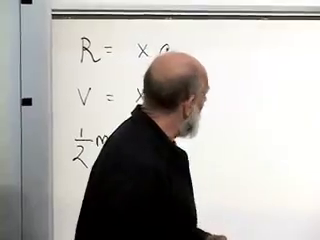
\includegraphics[width=0.72\textwidth]{lecture_09_figure_02.png}
  \caption{平直膨脹度規，標度因子乘上歐幾里得空間線元。來源畫面時間：00:09:12。}
  \label{fig:l09-expanding-metric-board}
\end{figure}

想像座標標記畫在一張橡膠片上。標記始終附著在橡膠片上，但標記之間的物理距離會逐漸增大。因此，像「從\(x=0\)到\(x=1\)」這樣的座標差只是一對標籤；這段間隔所代表的距離是\(a(t)\)。找出支配這個標度因子的方程，就是本講座要探討的動力學問題。

\section{閉合、平直與開放的空間幾何}

平直性是觀測上的簡化，並非均勻性的必然結果。均勻且各向同性的空間幾何有三種：正曲率、零曲率和負曲率。要理解正曲率的情形，必須仔細區分維度。

軌跡
\begin{equation}
  X_1^2+X_2^2=R^2
\end{equation}
是一個圓，也就是一維球面\(S^1\)。它所包圍的內部是圓盤，也稱為二維球。增加一個嵌入座標，就得到
\begin{equation}
  X_1^2+X_2^2+X_3^2=R^2,
\end{equation}
普通的二維球面\(S^2\)。再增加第四個嵌入座標，就得到
\begin{equation}
  X_1^2+X_2^2+X_3^2+X_4^2=R^2,
  \label{eq:l09-three-sphere}
\end{equation}
三維球面\(S^3\)；它本身是三維空間。我們無法想像它嵌入四維空間的樣子，但其內在幾何並不需要這種嵌入才能存在。

\begin{figure}[H]
  \centering
  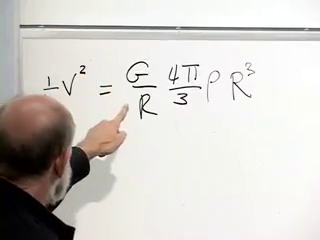
\includegraphics[width=0.72\textwidth]{lecture_09_figure_03.png}
  \caption{用來引介三維球面的嵌入方程。來源畫面時間：00:16:40。}
  \label{fig:l09-three-sphere-board}
\end{figure}

理想球面上的每一點在幾何上都與其他點等價，而每一點上的各個方向也都等價。因此，球面既均勻又各向同性。如果半徑乘上\(a(t)\)，整個空間便會膨脹或收縮，卻不會在球面上選出某個中心。將這樣的宇宙往回追溯，並不會把所有物質都放到外部虛空中的某個特殊位置。整個空間都會縮小，因此任意兩點都會彼此接近。大爆炸並不是從空間中的某一點向外爆炸。

在正曲率球面上，測地三角形的內角和大於
\(180^\circ\)。平直三角形的內角和恰好等於\(180^\circ\)。在均勻的負曲率幾何中，內角和小於\(180^\circ\)；馬鞍面只是對這種幾何不完全準確的示意。這些內在幾何檢驗可以區分這三種情形。

\begin{figure}[H]
  \centering
  \includegraphics[width=0.72\textwidth]{lecture_09_figure_07.png}
  \caption{以各自特有的三角形形狀示意正曲率、零曲率與負曲率。來源畫面時間：00:37:30。}
  \label{fig:l09-curvature-board}
\end{figure}

局部度規完全平直，本身並不能證明空間在拓撲上是無限的。數學上也可能存在緊緻的平直拓撲，不過本講座採用最簡單的無限歐幾里得模型。
\editorialnote{這項關於整體拓撲的限定，對後續任何局部動力學都沒有必要。}

\section{共動標籤與哈伯定律}

現在回到膨脹的平直薄片，在上面畫出座標網格。在共動座標中，網格隨著大尺度物質流一起膨脹。星系，或更精確地說，足夠粗粒化後的星系團，會維持近似固定的座標標籤，即使它與另一個共動物體之間的物理距離正在改變。

\begin{figure}[H]
  \centering
  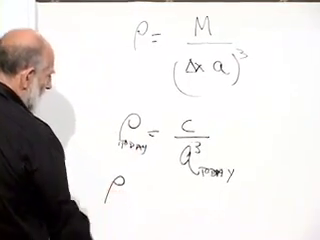
\includegraphics[width=0.72\textwidth]{lecture_09_figure_04.png}
  \caption{隨膨脹的空間薄片一起伸展的座標網格。來源畫面時間：00:22:20。}
  \label{fig:l09-comoving-grid-board}
\end{figure}

兩個物體沿\(x\)軸相隔固定的共動間隔\(\Delta x\)，其物理距離為
\begin{equation}
  D(t)=a(t)\,\Delta x.
  \label{eq:l09-physical-distance}
\end{equation}
保持\(\Delta x\)不變並對時間微分，得到
\begin{equation}
  v(t)=\dot a(t)\,\Delta x
      =\frac{\dot a(t)}{a(t)}D(t).
\end{equation}
定義
\begin{equation}
  H(t)\equiv\frac{\dot a(t)}{a(t)},
  \label{eq:l09-hubble-parameter}
\end{equation}
便得到哈伯定律：
\begin{equation}
  v=H(t)D.
  \label{eq:l09-hubble-law}
\end{equation}
「哈伯常數」中的「常數」，是指在指定的宇宙時刻，這個量在空間各處都相同；這不表示它在整個宇宙歷史中保持不變。

\begin{figure}[H]
  \centering
  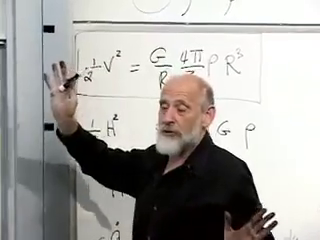
\includegraphics[width=0.72\textwidth]{lecture_09_figure_05.png}
  \caption{黑板上的推導：\(D=a\Delta x\)，
  \(v=(\dot a/a)D=HD\)。來源畫面時間：00:26:40。}
  \label{fig:l09-hubble-board}
\end{figure}

\begin{classroomqa}
\audiencequestion{如果我們看到一個遙遠星系的時間較早，推得的哈伯參數真的應該等於今天在附近測得的值嗎？}
\lecturerresponse{只有當回溯時間相較於宇宙年齡很短時，才是如此。在不太遠的距離上，\(H(t)\)的變化不大，因此用單一數值仍然合適。到了真正的宇宙學距離，我們看到的是較早的宇宙時期，就必須納入\(a\)和\(H\)隨時間變化的影響。這也是我們需要標度因子動力學方程的原因之一。}
\end{classroomqa}

\section{膨脹座標系中的零測地線}

\begin{classroomqa}
\audiencequestion{標度因子會影響光在遙遠星系之間的傳播嗎？}
\lecturerresponse{光線沿著零測地線傳播，因此\(d\tau=0\)。對於沿正\(x\)軸傳播的光線，\(dy=dz=0\)，膨脹度規給出
\begin{align}
  0&=dt^2-a^2(t)dx^2,
  &dt&=a(t)dx,\notag\\
  &&\frac{dx}{dt}&=\frac{1}{a(t)}.
  \label{eq:l09-null-ray}
\end{align}
隨著\(a(t)\)增大，座標速度會降低，但光的局部物理速度仍為\(c=1\)。固定的座標間隔所代表的物理距離則會逐漸增加。}
\end{classroomqa}

\begin{figure}[H]
  \centering
  \includegraphics[width=0.72\textwidth]{lecture_09_figure_06.png}
  \caption{徑向光傳播的零條件與\(dt=a(t)dx\)。來源畫面時間：00:30:54。}
  \label{fig:l09-null-board}
\end{figure}

我們可以選擇一套座標，讓同一件事聽起來像是「光在較遠處變慢了」，但相應地，長度和時鐘的描述也會變得彆扭。以空間膨脹來描述更簡潔，因為這保留了局部的陳述：每位自由落下的觀測者測得的光速都相同。

\begin{classroomqa}
\audiencequestion{有證據顯示，遙遠星系中的局部光傳播和原子物理與我們這裡相同嗎？}
\lecturerresponse{只有無量綱的比較才具有可操作的意義。選定一種原子尺度作為長度單位，再選定原子或核子的週期作為時間單位，接著詢問光穿越所選長度需要多少個這樣的週期。光譜觀測支持這項說法：這些無量綱比值在遙遠區域也相同。證據雖然是間接的，但這正是檢驗局部定律是否一致的一類比較。}
\end{classroomqa}

當可觀測宇宙極其微小時，光可以在相應的光穿越時間內迅速穿過一個給定的物理區域。這並不表示\(c\)有所不同，而是表示該區域本身很小。

\section{宇宙中的牛頓球體}

現在我們從運動學轉向動力學。以我們所在的位置為原點，畫出一個足以容納許多星系和星系團的大球，並在球面上選取一個星系。在均勻宇宙中，質量分布以我們為中心呈球對稱；牛頓殼層定理給出兩個關鍵事實：
\begin{enumerate}
  \item 所選半徑以外的球對稱物質，對球面上的星系施加的牛頓合力為零；
  \item 球內所有物質對這種徑向運動的作用，都等同於集中在球心。
\end{enumerate}
我們採用一個自身靜止的參考系，因此以下論證中的速度和加速度都是相對於我們測量的。

\begin{figure}[H]
  \centering
  \includegraphics[width=0.72\textwidth]{lecture_09_figure_08.png}
  \caption{殼層定理的構造：我們位於中心，測試星系位於大型均勻球體的邊界。來源畫面時間：00:41:10。}
  \label{fig:l09-shell-board}
\end{figure}

\begin{figure}[H]
  \centering
  \begin{tikzpicture}[scale=0.92,>=Latex]
    \draw[thick] (0,0) circle (2.35);
    \fill (0,0) circle (2pt) node[below left] {us};
    \fill (2.35,0) circle (2.2pt) node[right] {test galaxy \(m\)};
    \draw[->,thick,blue!65!black] (0.18,0) -- (2.15,0)
      node[midway,above] {\(R=a(t)x\)};
    \draw[->,thick,red!65!black] (2.35,0.12) -- (3.25,0.12)
      node[midway,above] {\(v=\dot a(t)x\)};
    \node[align=center,text width=7cm] at (0,-2.85)
      {outside shells cancel;\\enclosed mass acts at the center};
  \end{tikzpicture}
  \caption{牛頓構造的清晰重繪。}
  \label{fig:l09-shell-clean}
\end{figure}

若星系的共動座標\(x\)固定，則其物理半徑和速度為
\begin{equation}
  R(t)=x a(t),
  \qquad
  v(t)=x\dot a(t)=H(t)R(t).
  \label{eq:l09-radius-velocity}
\end{equation}
令\(M\)為球體所包圍的質量，\(m\)為測試星系的質量。牛頓能量為
\begin{equation}
  E=\frac12 m v^2-\frac{GMm}{R}.
  \label{eq:l09-newtonian-energy}
\end{equation}

\begin{figure}[H]
  \centering
  \includegraphics[width=0.72\textwidth]{lecture_09_figure_09.png}
  \caption{完整的板書推導：\(R=xa\)、\(v=x\dot a\)，以及針對\(E=0\)的牛頓能量方程。來源畫面時間：00:48:40。}
  \label{fig:l09-energy-board}
\end{figure}

能量可以是正、零或負。我們先從逃逸與再坍縮之間的邊界情形\(E=0\)開始，此時
\begin{equation}
  \frac12 v^2=\frac{GM}{R}.
  \label{eq:l09-zero-energy}
\end{equation}

\begin{classroomqa}
\audiencequestion{退行星系的總能量為零，代表什麼？}
\lecturerresponse{這正是達到逃逸速度的情形。正能量表示速度高於逃逸速度；負能量表示速度低於逃逸速度，在只有物質的牛頓圖像中，星系最終會返回。我們先從兩種可能性之間的邊界推導，得到平直方程後再回頭討論另外兩種能量符號。}
\end{classroomqa}

\begin{classroomqa}
\audiencequestion{球體膨脹時，所包圍的質量\(M\)會改變嗎？}
\lecturerresponse{不會。球體是共動的，因此相同的粒子會一直留在其中。球體的物理體積增大，密度下降，但所包圍的總質量不變。\(M\)與\(\rho(t)\)的區別至關重要。}
\end{classroomqa}

對於均勻密度\(\rho(t)\)，
\begin{equation}
  M=\frac{4\pi}{3}\rho(t)R^3.
  \label{eq:l09-enclosed-mass}
\end{equation}
代入\eqref{eq:l09-zero-energy}，得到
\begin{equation}
  \frac12 v^2
  =\frac{G}{R}\left(\frac{4\pi}{3}\rho R^3\right).
  \label{eq:l09-enclosed-energy}
\end{equation}

\begin{figure}[H]
  \centering
  \includegraphics[width=0.72\textwidth]{lecture_09_figure_10.png}
  \caption{將所包圍質量代入零能量方程。來源畫面時間：00:54:16.060。}
  \label{fig:l09-enclosed-mass-board}
\end{figure}

利用\(v=HR\)，得到
\begin{align}
  \frac12 H^2R^2
    &=\frac{4\pi G}{3}\rho R^2,\\
  H^2
    &=\frac{8\pi G}{3}\rho.
\end{align}
因此，零能量、空間平直的膨脹定律為
\begin{equation}
  \boxed{\left(\frac{\dot a}{a}\right)^2
  =\frac{8\pi G}{3}\rho(t)}.
  \label{eq:l09-flat-friedmann}
\end{equation}
消去\(R^2\)並非偶然。無論選哪個共動星系作為測試物體，均勻宇宙都必須給出相同的\(H(t)\)。

\begin{figure}[H]
  \centering
  \includegraphics[width=0.72\textwidth]{lecture_09_figure_11.png}
  \caption{板書展示了半徑的消去，以及由此得到的平直弗里德曼關係。來源畫面時間：00:57:30。}
  \label{fig:l09-friedmann-board}
\end{figure}

\begin{classroomqa}
\audiencequestion{有證據支持零能量關係嗎？}
\lecturerresponse{等式兩邊都可以由觀測推得：\(H\)來自退行資料，而\(\rho\)則是將恆星、氣體、暗物質和真空能都納入計算後得到的。講座當時的比較顯示，兩邊在約百分之幾的精度內一致。這項限定很重要：必須計入所有形式的能量，而且後面對真空能的討論會修正對逃逸速度的直觀解讀。}
\end{classroomqa}

在\(c=1\)的單位制下，質量密度和能量密度的單位相同。因此，符號\(\rho\)將表示所討論組分對應的總能量密度。

\section{普通物質與三分之二次方定律}

在知道\(\rho(t)\)如何變化之前，方程\eqref{eq:l09-flat-friedmann}還不是封閉的。先用緩慢運動的非相對論粒子填滿一個共動長方體。它的座標尺寸固定，物理體積則按下式增大：
\begin{equation}
  V(t)=a^3(t)\,\Delta x\,\Delta y\,\Delta z.
\end{equation}
盒中的粒子數和靜止質量維持不變，因此
\begin{equation}
  \rho_{\mathrm m}(t)=\frac{C_{\mathrm m}}{a^3(t)}.
  \label{eq:l09-matter-dilution}
\end{equation}
以目前時期\(t_0\)為基準正規化，得到
\begin{equation}
  \frac{\rho_{\mathrm m}(t)}{\rho_{\mathrm m,0}}
  =\left(\frac{a_0}{a(t)}\right)^3.
  \label{eq:l09-matter-normalized}
\end{equation}

\begin{figure}[H]
  \centering
  \includegraphics[width=0.72\textwidth]{lecture_09_figure_12.png}
  \caption{物質密度按\(a^{-3}\)稀釋，以及以現在為基準的正規化。來源畫面時間：01:04:47.940。}
  \label{fig:l09-density-board}
\end{figure}

\begin{classroomqa}
\audiencequestion{目前宇宙的能量密度大約是多少？只靠普通原子能提供這麼多能量嗎？}
\lecturerresponse{只計算可見的重子物質，並不足以回答這個問題。暗物質和暗能量也必須以等效質能計入。講座引用的粗略範圍是每立方公尺相當於一個原子至數十個氫原子的質量，強調的是數量級，而非精確盤點。}
\end{classroomqa}

將\eqref{eq:l09-matter-dilution}代入\eqref{eq:l09-flat-friedmann}，並把所有與時間無關的因子吸收到一個正的常數\(C\)中：
\begin{equation}
  \left(\frac{\dot a}{a}\right)^2=\frac{C}{a^3},
  \qquad
  \dot a^2=\frac{C}{a}.
  \label{eq:l09-matter-ode}
\end{equation}
求解有兩種直接的方法。假設冪律形式\(a=K t^p\)，便須滿足
\begin{equation}
  p-1=-\frac{p}{2},
  \qquad p=\frac23.
\end{equation}
另一種等價的做法是取膨脹解的平方根分支並積分：
\begin{equation}
  a^{1/2}\frac{da}{dt}=\sqrt C,
  \qquad
  \int a^{1/2}da=\sqrt C\int dt,
\end{equation}
因此，選定大爆炸時刻為時間原點後，
\begin{equation}
  a^{3/2}\propto t,
  \qquad
  \boxed{a(t)\propto t^{2/3}}.
  \label{eq:l09-matter-solution}
\end{equation}
現場推導在配對係數時一度漏掉一個因子，之後回到積分重新檢查指數。筆記保留了這項檢查，但只列出修正後的代數推導。

\begin{figure}[H]
  \centering
  \includegraphics[width=0.72\textwidth]{lecture_09_figure_13.png}
  \caption{冪律假設與框出的指數\(p=2/3\)。來源畫面時間：01:13:05。}
  \label{fig:l09-matter-solution-board}
\end{figure}

對解微分，得到
\begin{equation}
  H(t)=\frac{\dot a}{a}=\frac{2}{3t}.
  \label{eq:l09-matter-hubble}
\end{equation}
過去的哈伯參數較大。因此，當觀測距離遠到足以涵蓋明顯的回溯時間時，不應把今天的\(H_0\)當成不變的數值，直接外推局部線性關係。

\begin{figure}[H]
  \centering
  \includegraphics[width=0.72\textwidth]{lecture_09_figure_14.png}
  \caption{將\(\dot a/a\)代入\(a\propto t^{2/3}\)，得到
  \(H=2/(3t)\)。來源畫面時間：01:20:42。}
  \label{fig:l09-hubble-time-board}
\end{figure}

\section{能量符號與空間曲率}

牛頓式推理帶領我們推導出平直、零能量的情形。廣義相對論還補充了一項僅靠殼層定理無法得到的事實：牛頓式比能量的正負，對應於空間曲率的正負。
\begin{center}
\begin{tabular}{@{}>{\raggedright\arraybackslash}p{0.20\linewidth}
                    >{\raggedright\arraybackslash}p{0.29\linewidth}
                    >{\raggedright\arraybackslash}p{0.37\linewidth}@{}}
  \toprule
  總能量&空間曲率&僅含物質時的演化\\
  \midrule
  正&負（開放）&永遠膨脹\\
  零&零（平直）&漸近於逃逸邊界\\
  負&正（閉合）&膨脹、轉向、再坍縮\\
  \bottomrule
\end{tabular}
\end{center}
最後一欄假設沒有真空能。在拋射體的類比中，正能量表示速度高於逃逸速度，零能量表示速度恰好等於逃逸速度，負能量則表示速度低於逃逸速度。愛因斯坦方程分別將這三種情形對應到開放、平直和閉合的空間幾何。

\section{光子與二分之一次方定律}

物質定律\(\rho\propto a^{-3}\)假設每個粒子的能量近似固定，而數密度逐漸下降。光子不符合這項假設。對光子而言，
\begin{equation}
  E=h\nu=\frac{hc}{\lambda}.
\end{equation}
宇宙膨脹會使波長按標度因子的比例伸長，
\begin{equation}
  \lambda\propto a,
  \qquad E\propto a^{-1}.
\end{equation}
光子數密度仍按\(a^{-3}\)下降，而每個光子的能量還會額外帶來一個\(a^{-1}\)因子。因此
\begin{equation}
  \boxed{\rho_{\mathrm r}(t)\propto a^{-4}(t)}.
  \label{eq:l09-radiation-dilution}
\end{equation}

吉他弦的類比呈現了這個物理圖像。先撥動琴弦，再拉長它振動的部分：波長變長，音調降低。膨脹共動盒中的光子模式也有類似的行為。反過來看，壓縮會縮短波長並提高光子能量。

\begin{figure}[H]
  \centering
  \includegraphics[width=0.72\textwidth]{lecture_09_figure_15.png}
  \caption{黑板上將物質密度關係推展至輻射的標度關係\(\rho_{\mathrm r}\propto a^{-4}\)。來源畫面時間：01:29:20。}
  \label{fig:l09-radiation-board}
\end{figure}

將\(\rho_{\mathrm r}\propto a^{-4}\)代入平直弗里德曼方程，得到
\begin{equation}
  \left(\frac{\dot a}{a}\right)^2=\frac{C_{\mathrm r}}{a^4},
  \qquad
  \dot a\propto a^{-1},
\end{equation}
因此
\begin{equation}
  \boxed{a(t)\propto t^{1/2}}.
  \label{eq:l09-radiation-solution}
\end{equation}
這比\(t^{2/3}\)的增長慢。回溯到足夠早的時期，輻射必定會主導普通物質，因為當\(a\)減小時，\(a^{-4}\)上升的速度比\(a^{-3}\)快。講座將物質與輻射的交會時期定在標度因子約比今天小一千倍的時候。在交會之前，宇宙由輻射主導；交會之後，則由物質主導了很長一段時間。

\section{真空能與指數膨脹}

真空能的標度行為正好相反。真空能密度是空無一物的空間所具有的性質，不會隨宇宙膨脹而稀釋：
\begin{equation}
  \rho_\Lambda=\text{constant}.
  \label{eq:l09-vacuum-density}
\end{equation}
普通物質和輻射在過去的密度較高，這一項則不會。因此，在早期宇宙中，真空能較不重要；隨著其他組分稀釋，它便愈來愈重要。講座採用當時的估計，認為真空能約占今日宇宙能量密度的\(70\%\)。

當\(\rho_\Lambda\)為常數時，方程\eqref{eq:l09-flat-friedmann}給出固定的膨脹率
\begin{equation}
  H_\Lambda=\sqrt{\frac{8\pi G}{3}\rho_\Lambda},
  \qquad
  \frac{\dot a}{a}=H_\Lambda.
\end{equation}
因此
\begin{equation}
  \boxed{a(t)=a(t_i)e^{H_\Lambda(t-t_i)}}.
  \label{eq:l09-vacuum-solution}
\end{equation}

\begin{figure}[H]
  \centering
  \includegraphics[width=0.72\textwidth]{lecture_09_figure_16.png}
  \caption{導出指數膨脹的定密度方程。來源畫面時間：01:35:48。}
  \label{fig:l09-vacuum-board}
\end{figure}

以講座引用的觀測尺度來看，宇宙的線性尺度約每一百億至一百二十億年加倍。這個微小但非零的真空能密度為何存在，至今仍無法解釋；它的存在及其對膨脹的影響則是經驗事實。

\begin{classroomqa}
\audiencequestion{在這段討論中，真空能和暗能量是同一回事嗎？}
\lecturerresponse{是的。這裡的「暗能量」指密度固定的真空能，等價於宇宙學常數。也可以設想更一般、隨時間變化的暗能量模型，但這些模型不在本講座的計算範圍內。}
\end{classroomqa}

\section{膨脹宇宙如何使光紅移}

\begin{classroomqa}
\audiencequestion{光子怎麼會知道我們選了膨脹的共動座標，因而降低自己的能量？}
\lecturerresponse{光子並不會對我們的標記作出反應。它們是在物理間隔不斷變化的幾何中傳播。若一列波佔據的區域，其物理尺度加倍，波長也會加倍。共動座標只是方便地描述這種伸長，並不會造成伸長。}
\end{classroomqa}

\begin{classroomqa}
\audiencequestion{今天抵達我們的背景光子來自何處？}
\lecturerresponse{看得愈遠，就看得愈早。最後，我們會看到宇宙物質處於電離電漿的時期；當時自由帶電粒子不斷散射光子，因此電漿是不透明的。光子最後一次能不受阻礙地傳到我們這裡的邊界，在觀測者周圍呈現為一個球面，稱為最後散射面。}
\end{classroomqa}

\begin{figure}[H]
  \centering
  \includegraphics[width=0.72\textwidth]{lecture_09_figure_17.png}
  \caption{以觀測者為中心的最後散射面，以及一層層愈來愈遠的殼層示意圖。來源畫面時間：01:42:05。}
  \label{fig:l09-last-scattering-board}
\end{figure}

\begin{figure}[H]
  \centering
  \begin{tikzpicture}[scale=0.9,>=Latex]
    \fill (0,0) circle (2pt) node[below] {observer};
    \draw[thick,orange!70!black] (0,0) circle (2.55);
    \node[orange!70!black,align=center] at (0,3.05)
      {surface of last scattering};
    \foreach \a in {25,75,145,210,285,335}{
      \draw[->,blue!60!black] ({2.55*cos(\a)},{2.55*sin(\a)}) --
        ({1.7*cos(\a)},{1.7*sin(\a)});
    }
    \draw[decorate,decoration={snake,amplitude=1.5pt,segment length=7pt},
      red!65!black,thick,->] (-2.5,0) -- (-0.15,0);
    \node[red!65!black,below] at (-1.35,-0.15)
      {redshifted photon};
  \end{tikzpicture}
  \caption{最後散射圖像的清晰重繪。}
  \label{fig:l09-last-scattering-clean}
\end{figure}

這些輻射發射時具有熱電漿的特徵光譜；抵達我們時，波長約增加了一千倍。用講座中的多普勒說法來描述，遙遠的發射面快速遠離，其輻射受到強烈紅移。用幾何說法來描述，波在傳播過程中被拉長。兩種圖像描述的是同一關係：
\begin{equation}
  1+z=\frac{\lambda_0}{\lambda_{\mathrm{em}}}
      =\frac{a_0}{a_{\mathrm{em}}}.
  \label{eq:l09-cosmological-redshift}
\end{equation}
\editorialnote{方程\eqref{eq:l09-cosmological-redshift}是講座中拉伸與多普勒描述的標準定量形式。}

若在較早的宇宙時期觀測，依照相應的圖像，最後散射面會比較近；觀測到的背景光子紅移也較小，因此能量較高。隨著宇宙時間推進，從早期電漿傳到共動觀測者的光子，其波長會逐漸變長。

\section{紅移後的光子能量去了哪裡？}

\begin{classroomqa}
\audiencequestion{光子發射時的能量是\(h\nu_{\mathrm{em}}\)，抵達時已紅移，能量也減少了。減少的能量去了哪裡？}
\lecturerresponse{牛頓推導一開始就是能量方程。其宇宙學形式將膨脹率與物質能量密度聯繫起來，因此不能把物質能量和膨脹視為各自守恆的帳目。講座將光子流失的能量描述為納入膨脹的動能帳目。以充滿輻射的活塞為例，這個類比就很具體：輻射壓將活塞向外推，光子的波長隨之增加，流失的能量則轉化為機械功和活塞的動能。}
\end{classroomqa}

\begin{figure}[H]
  \centering
  \includegraphics[width=0.72\textwidth]{lecture_09_figure_18.png}
  \caption{黑板上將框起來的牛頓能量方程置於相應的弗里德曼方程上方。來源畫面時間：01:44:42。}
  \label{fig:l09-energy-bookkeeping-board}
\end{figure}

\begin{classroomqa}
\audiencequestion{是什麼讓輻射能量與膨脹耦合？}
\lecturerresponse{壓力。在裝有可移動活塞的圓筒中，光子會把動量傳給壁面。活塞移動時，輻射便做功；光子的波長增加，能量則降低。均勻膨脹的宇宙並沒有字面意義上的外部活塞，但\(p\,dV\)類比說明了為何輻射能量密度的下降速度，會快於單靠粒子數稀釋所造成的下降。}
\end{classroomqa}

\begin{figure}[H]
  \centering
  \includegraphics[width=0.72\textwidth]{lecture_09_figure_19.png}
  \caption{用來呈現壓力做功的可移動光子活塞。來源畫面時間：01:46:40。}
  \label{fig:l09-piston-board}
\end{figure}

\begin{figure}[H]
  \centering
  \begin{tikzpicture}[scale=0.92,>=Latex]
    \draw[thick] (0,0) rectangle (5.3,2.6);
    \draw[very thick] (4.25,0) -- (4.25,2.6);
    \draw[very thick] (4.25,1.3) -- (5.25,1.3);
    \draw[->,thick,red!65!black] (5.25,1.3) -- (6.2,1.3)
      node[right] {moving piston};
    \foreach \y in {0.55,1.3,2.05}{
      \draw[decorate,decoration={snake,amplitude=1.4pt,segment length=6pt},
        blue!65!black,->] (0.35,\y) -- (3.9,\y);
    }
    \node at (2.15,-0.45) {radiation does \(p\,dV\) work};
  \end{tikzpicture}
  \caption{輻射與活塞類比的清晰重繪。}
  \label{fig:l09-piston-clean}
\end{figure}

廣義相對論中的能量需要謹慎處理。在一般的膨脹時空中，未必存在唯一的守恆全域能量，可與孤立牛頓系統的能量相類比。局域的應力—能量守恆仍然成立；對均勻流體而言，它導出連續性方程
\begin{equation}
  \dot\rho+3H(\rho+p)=0,
  \label{eq:l09-continuity}
\end{equation}
其中包含壓力做功項，這正是物質與輻射標度律的由來。\editorialnote{方程 \eqref{eq:l09-continuity} 是局域廣義相對論的精確表述，也是講座中刻意採用牛頓式能量收支類比的依據。}

真空能使這個問題格外尖銳。由於其密度保持不變而體積持續增大，共動區域內的真空能總量便會增加。真空能的負壓是引力源的一部分，並會驅動加速膨脹。因此，若不把幾何與壓力做功納入考量，就不應要求樸素理解下「共動盒中的物質能量」單獨守恆。

\section{為什麼時間項中的標度因子可以消去}

\begin{classroomqa}
\audiencequestion{為什麼標度因子乘在度規的空間部分上，卻沒有乘在時間部分上？}
\lecturerresponse{這是時間座標的選擇。假設一開始採用共形時間座標 \(t\)，度規為
\begin{equation}
  d\tau^2=A^2(t)\left(dt^2-dx^2\right).
\end{equation}
再以下式定義新的宇宙時間 \(T\)：
\begin{equation}
  dT=A(t)\,dt.
\end{equation}
則有
\begin{equation}
  d\tau^2=dT^2-A^2\bigl(t(T)\bigr)dx^2.
\end{equation}
時間微分前的共同因子便消去了，而物理標度因子仍留在空間項中。}
\end{classroomqa}

\begin{figure}[H]
  \centering
  \includegraphics[width=0.72\textwidth]{lecture_09_figure_20.png}
  \caption{將共形時間轉換為宇宙時間的時間座標重新定義 \(dT=A(t)dt\)。來源影格時間為 01：51：05。}
  \label{fig:l09-time-reparam-board}
\end{figure}

\section{曲率、真空能與宇宙的命運}

\begin{classroomqa}
\audiencequestion{如果宇宙具有正曲率，我們現在應該已經看到星系朝我們移動嗎？}
\lecturerresponse{未必。以低於逃逸速度發射的拋射體會先向外運動，到達轉折點後才落回。我們觀測到的宇宙正處於膨脹階段。若沒有真空能，正曲率的物質宇宙最終會再坍縮。若正值真空能足夠大，就能阻止宇宙在轉折點折返；觀測到的真空能值似乎大到足以使宇宙長期持續指數式膨脹，即使空間曲率很小也是如此。}
\end{classroomqa}

指數式膨脹的未來並非能量天堂。恆星終將燃盡，物質與輻射的密度會呈指數式下降，遙遠區域也會超出彼此的因果聯繫範圍。真空能依然存在，而一般結構則會逐漸變得更冷、更稀薄。

\begin{classroomqa}
\audiencequestion{愈往過去追溯，光子會比一般粒子更多嗎？}
\lecturerresponse{光子數與重子數之比早已極大；依照講座中的估計，每個重子約有 \(10^{10}\) 個光子，而共動體積內的這兩種粒子數都近似保持不變。往過去追溯時，主要改變的是每個光子的能量。光子能量會按 \(a^{-1}\) 增加，非相對論性粒子的靜止質量則不會。因此，即使粒子數之比本身未必改變，輻射在早期仍會主導能量密度。}
\end{classroomqa}

核心教訓是，單靠幾何並不能決定宇宙的演化歷史。平坦的弗里德曼方程給出膨脹與能量密度之間的關係，而物質成分則決定它們如何隨時間變化。非相對論性物質使 \(a\propto t^{2/3}\)，輻射使 \(a\propto t^{1/2}\)，恆定的真空能則導致指數式膨脹。這三條定律勾勒出宇宙各個相繼的時代，也說明了為什麼同一個標度因子會支配距離、紅移與哈勃參數的變化。

\end{document}